\chapter{All-Channel Archive Diagnostics}
\label{app:archive-diagnostics}

This appendix places the same diagnostic construction beside every physical
ATSC channel so that a reader does not have to infer the behaviour of the
lower band from a few selected examples.  The plates are generated in
PilotProxy from the 23 supplied per-pilot products after applying
\texttt{pilotproxy\_archive\_frame\_health\_gate\_v1}.  They are therefore
views of one frozen estimand: the trigger-selected archive after removal of
the four detector-invalid rows and 178 constant negative-full-scale rows.
They are not samples from a uniform observing calendar, and a blank month in a
plate means that the archive supplied no health-included frame in that month;
it does not establish that the television allocation was quiet.

Each plate has three layers.  The four upper panels are logarithmic-count
histograms over health-included frames.  From upper left to lower right they
show the coarse power ratio divided by the static weight-norm scale $\mu_0$,
the same coarse statistic expressed in the analyzer's normalized-decibel
coordinate, decoded native-complex-\texttt{int4} mean input power, and the
selected fine-window peak divided by its retrospective floating-point CFAR
threshold.  The selection has two explicit evidence states.  In a UTC quarter
with at least 30 health-included frames and a persistent, separated line inside
the geometry-predicted acquisition neighbourhood, it uses the narrow
$f_a\mathbin{\pm}2$ measured-line window.  Otherwise it refuses the narrow
anchor and falls back to the broad
$f_{\rm pred}\mathbin{\pm}30$-bin acquisition neighbourhood.  That broad
neighbourhood repairs the archived bin-zero mistake and is deliberately wide
enough to find a station-offset line; a stronger feature outside it is recorded
as a sentinel rather than allowed to redefine the target.  The orange reference lines mark
$F/\mu_0=1$, $0$~dB, and a fine peak-to-threshold ratio of one.  As explained
in Chapter~\ref{sec:pipeline:decision}, $\mu_0$ is the ratio-of-expected-powers
scale under the declared white/isotropic model, not an assertion that every
finite-sample null distribution has mean one.  Likewise, the fine ratio is a
diagnostic reconstructed from the retained 256-bin floating-point array.  The
quarterly partition, persistence cut, and threshold are retrospective analysis
choices made after this archive had been inspected.  They expose measured and
refused anchor states but do not constitute a prospective per-epoch Q16
calibration or blocked holdout.  In particular, channel 23's weak,
epoch-dependent structure is a measurement/refusal case rather than a reason
to widen the final decision silently.

The middle panel is a relative time-averaged spectrum before and after the
stored coarse mask.  Each accumulator is divided by its own contributing-frame
count and expressed in decibels relative to the median positive bin of the
health-corrected before-mask spectrum.  Consequently it exposes spectral
shape, lines, and the change induced by the stored mask, but it is neither an
absolutely calibrated power spectral density nor a quantity in watts per hertz.
The dashed orange line is the nominal received pilot frequency.  The title
reports how many constant-ceiling frames were subtracted from the before and
after accumulators.  For channels 22 and 24, no health-included frame survives
the stored mask, so an after-mask spectral shape is unavailable rather than a
zero-power measurement.

The lower panel is the closest time--frequency diagnostic supported by the
saved products.  It is the arithmetic mean of the fine-stage $F$ statistic in
each UTC calendar month, displayed as $10\log_{10}F$ against fine-envelope
frequency.  The dashed white line is the geometry-predicted pilot anchor;
orange quarter-length segments mark only the measured narrow anchors that pass
the declared persistence and separation gates, and calendar gaps remain
visible.  This panel is deliberately labelled a
detector-statistic heatmap: the archive does not retain a voltage spectrum for
each frame, so it cannot supply a raw-voltage spectrogram or support arbitrary
post-hoc spectral remasking.  These distinctions are part of the evidence,
not merely plotting qualifications.

Table~\ref{tab:archive:atlas-counts} gives the denominator of every plate.  The
last column counts health-included frames that the historical stored coarse
mask kept; it is not a final recommended operating point.  Its two zeros are
scientifically consequential: the apparent kept populations of channels 22
and 24 consisted entirely of the subsequently identified constant-ceiling
rows.  Those channels therefore have no archive-derived after-mask floor under
that decision and must be treated as unavailable/excision candidates unless a
new clean population or independently justified synthetic bound is supplied.

\begin{landscape}
\begin{table}[p]
\centering
\caption{Per-channel denominators for the archive diagnostic plates.  ``Kept''
means retained by both the v1 input-health gate and the stored historical
coarse mask.}
\label{tab:archive:atlas-counts}
\small
\begin{tabular}{rrrrr@{\qquad}rrrrr}
\toprule
Channel & \texttt{freq\_id} & Health frames & Excluded & Kept &
Channel & \texttt{freq\_id} & Health frames & Excluded & Kept \\
\midrule
14 & 844 & 35,023 & 7 & 1,836 & 26 & 660 & 26,348 & 4 & 1,234 \\
15 & 829 & 34,213 & 7 & 26 & 27 & 644 & 34,542 & 7 & 666 \\
16 & 813 & 36,367 & 18 & 3,057 & 28 & 629 & 32,816 & 13 & 71 \\
17 & 798 & 33,190 & 9 & 32 & 29 & 614 & 39,350 & 7 & 14,274 \\
18 & 783 & 38,067 & 6 & 2,909 & 30 & 598 & 9,289 & 0 & 148 \\
19 & 767 & 21,362 & 10 & 1,752 & 31 & 583 & 30,985 & 7 & 6 \\
20 & 752 & 36,727 & 9 & 70 & 32 & 568 & 28,209 & 6 & 8,154 \\
21 & 736 & 38,614 & 8 & 15,578 & 33 & 552 & 34,200 & 6 & 6,653 \\
22 & 721 & 37,959 & 7 & 0 & 34 & 537 & 39,012 & 5 & 355 \\
23 & 706 & 37,675 & 7 & 4,255 & 35 & 521 & 39,767 & 8 & 6,476 \\
24 & 690 & 10,152 & 2 & 0 & 36 & 506 & 38,155 & 5 & 29 \\
25 & 675 & 38,257 & 24 & 4,228 & Total & --- & 750,279 & 182 & 71,809 \\
\bottomrule
\end{tabular}
\end{table}
\end{landscape}

\clearpage
\section{Per-channel plates}

The plates follow increasing physical-channel order.  Reading them in this
order is useful because adjacent physical allocations do not map to adjacent
CHIME \texttt{freq\_id} values: the latter decreases as sky frequency
increases.  Channel 14 also exercises the circular fine-bin convention at the
edge of the fine transform.  No plate recentres that case for visual
convenience; the same geometry function used by the analysis supplies the
dashed anchor.

\begin{figure}[p]
\centering
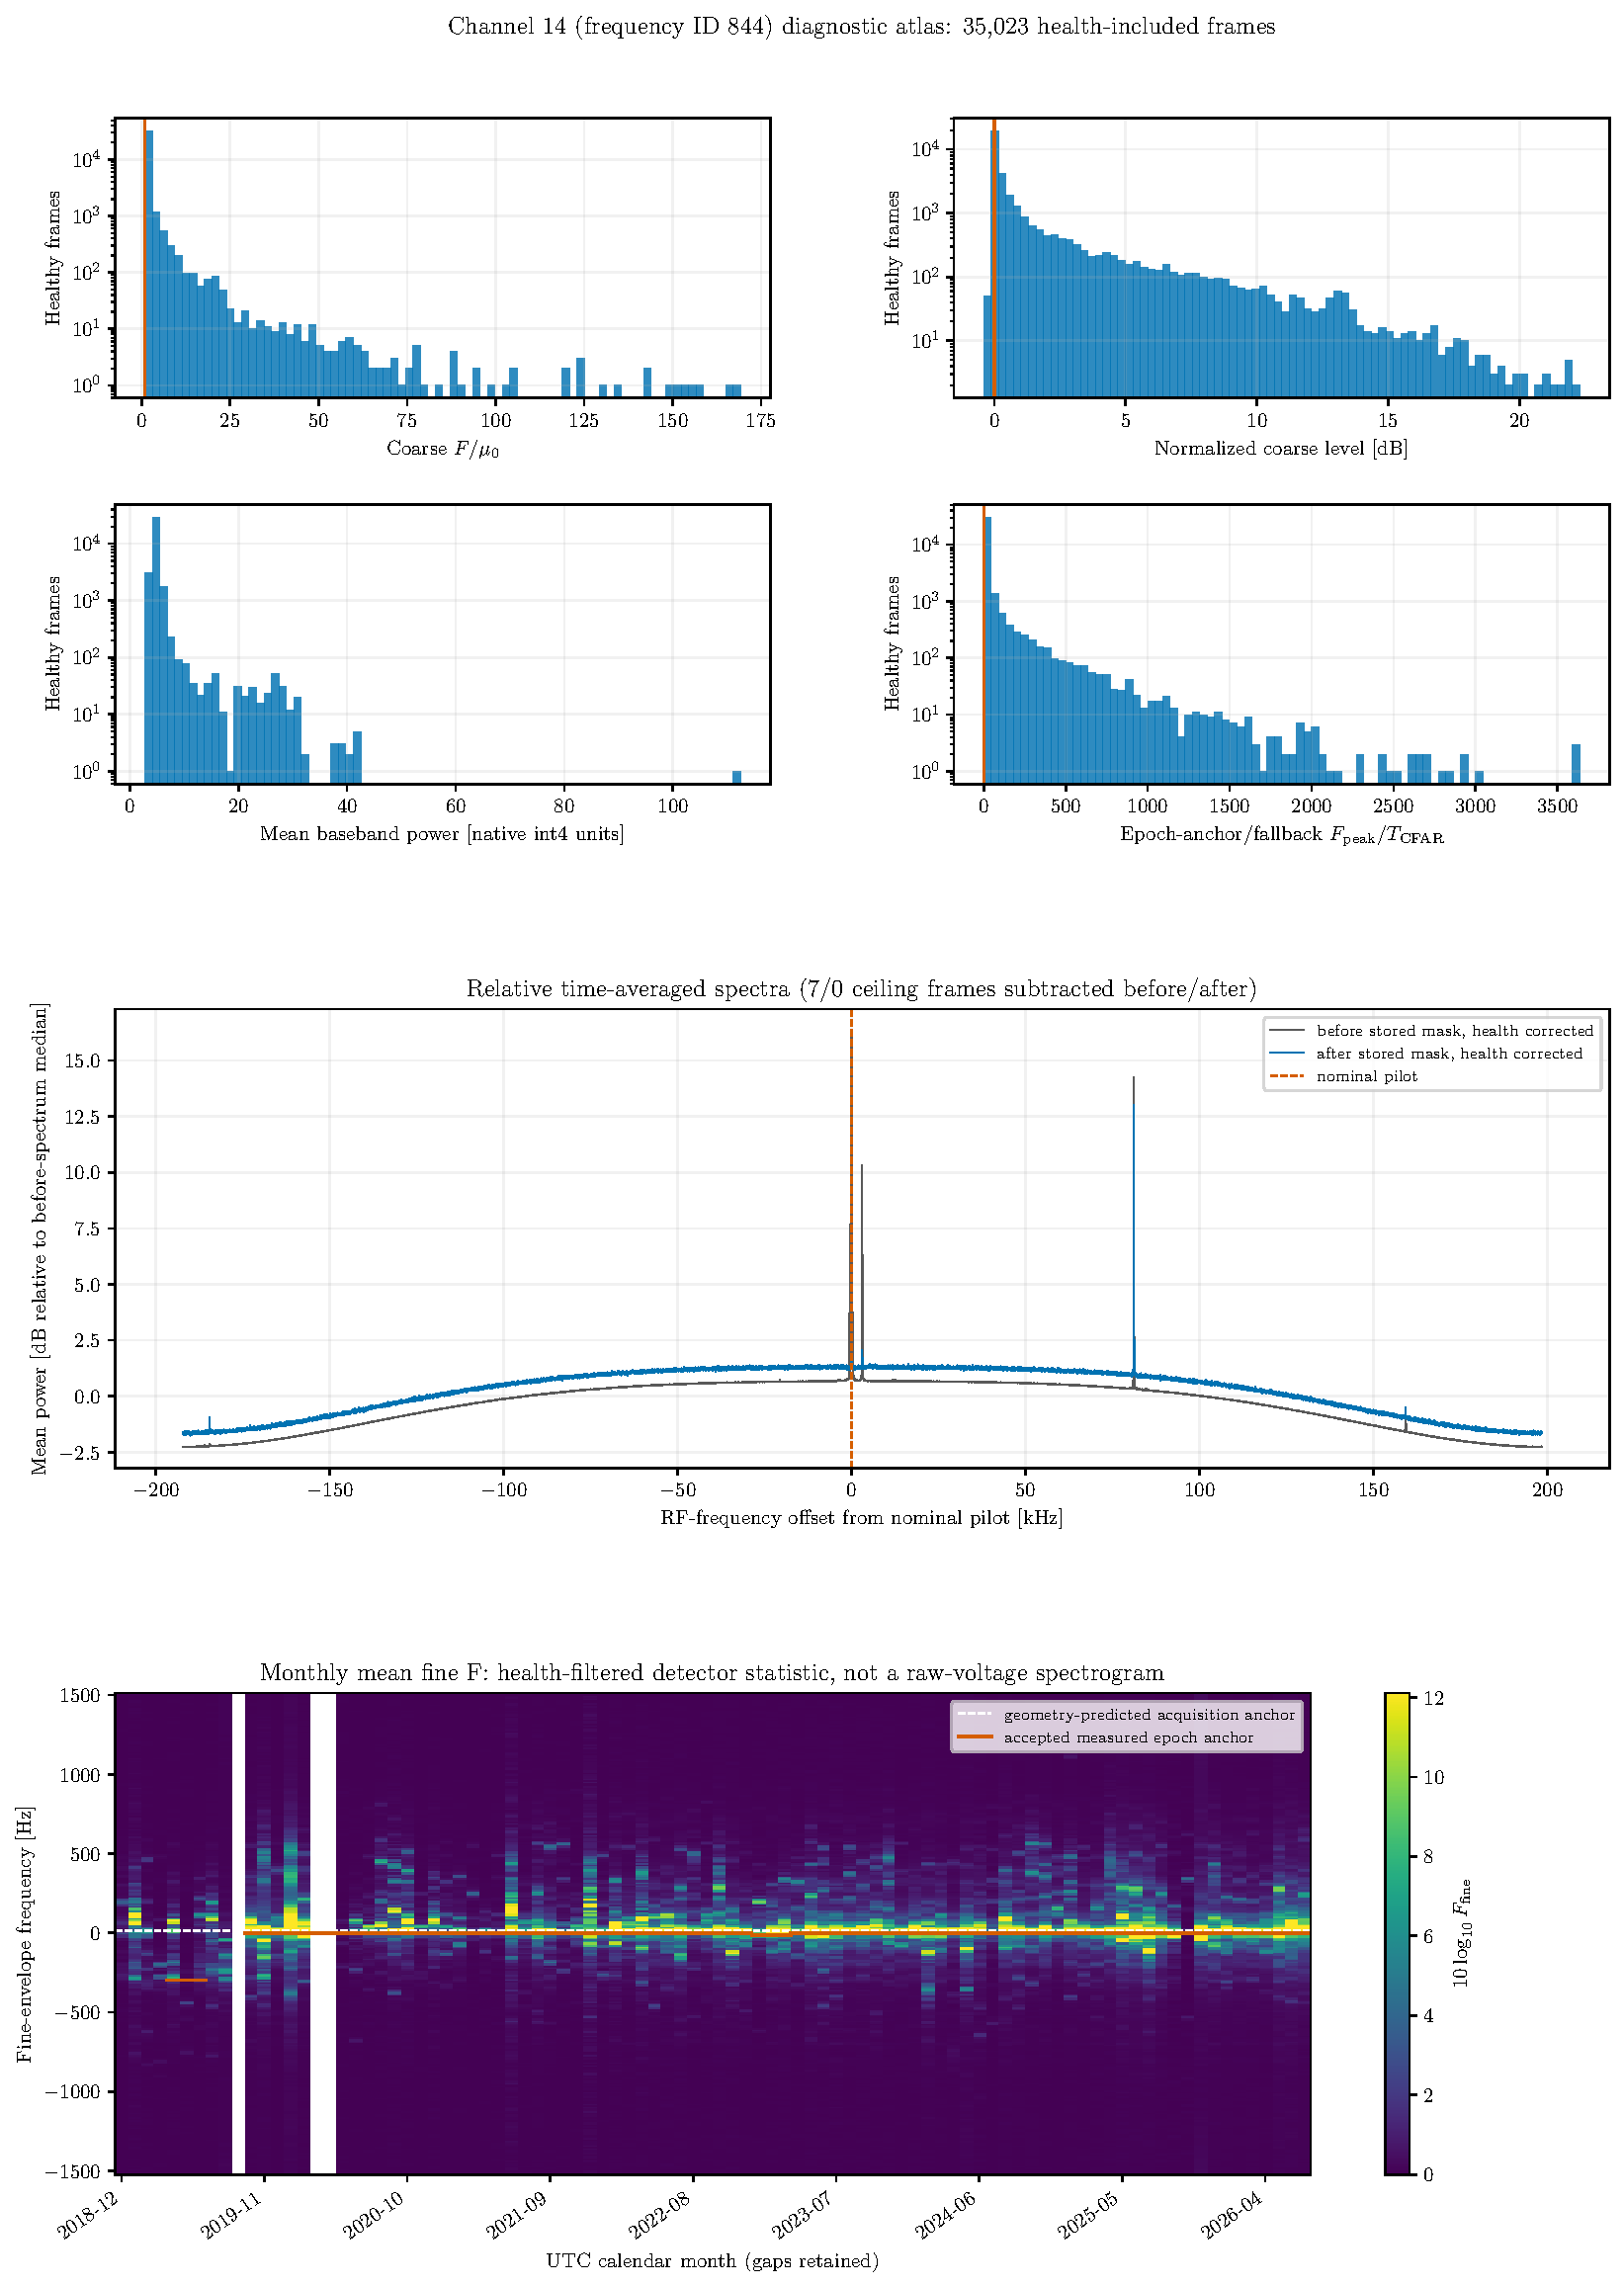
\includegraphics[width=0.98\linewidth,height=0.82\textheight,keepaspectratio]{figs/archive_health_v1/channel_14_diagnostic_atlas.pdf}
\caption{Channel 14 (\texttt{freq\_id}=844).  This band-edge case exercises the circular fine-window convention; seven ceiling frames are removed before the stored mask and none after it.}
\label{fig:archive:atlas:14}
\end{figure}
\clearpage

\begin{figure}[p]
\centering
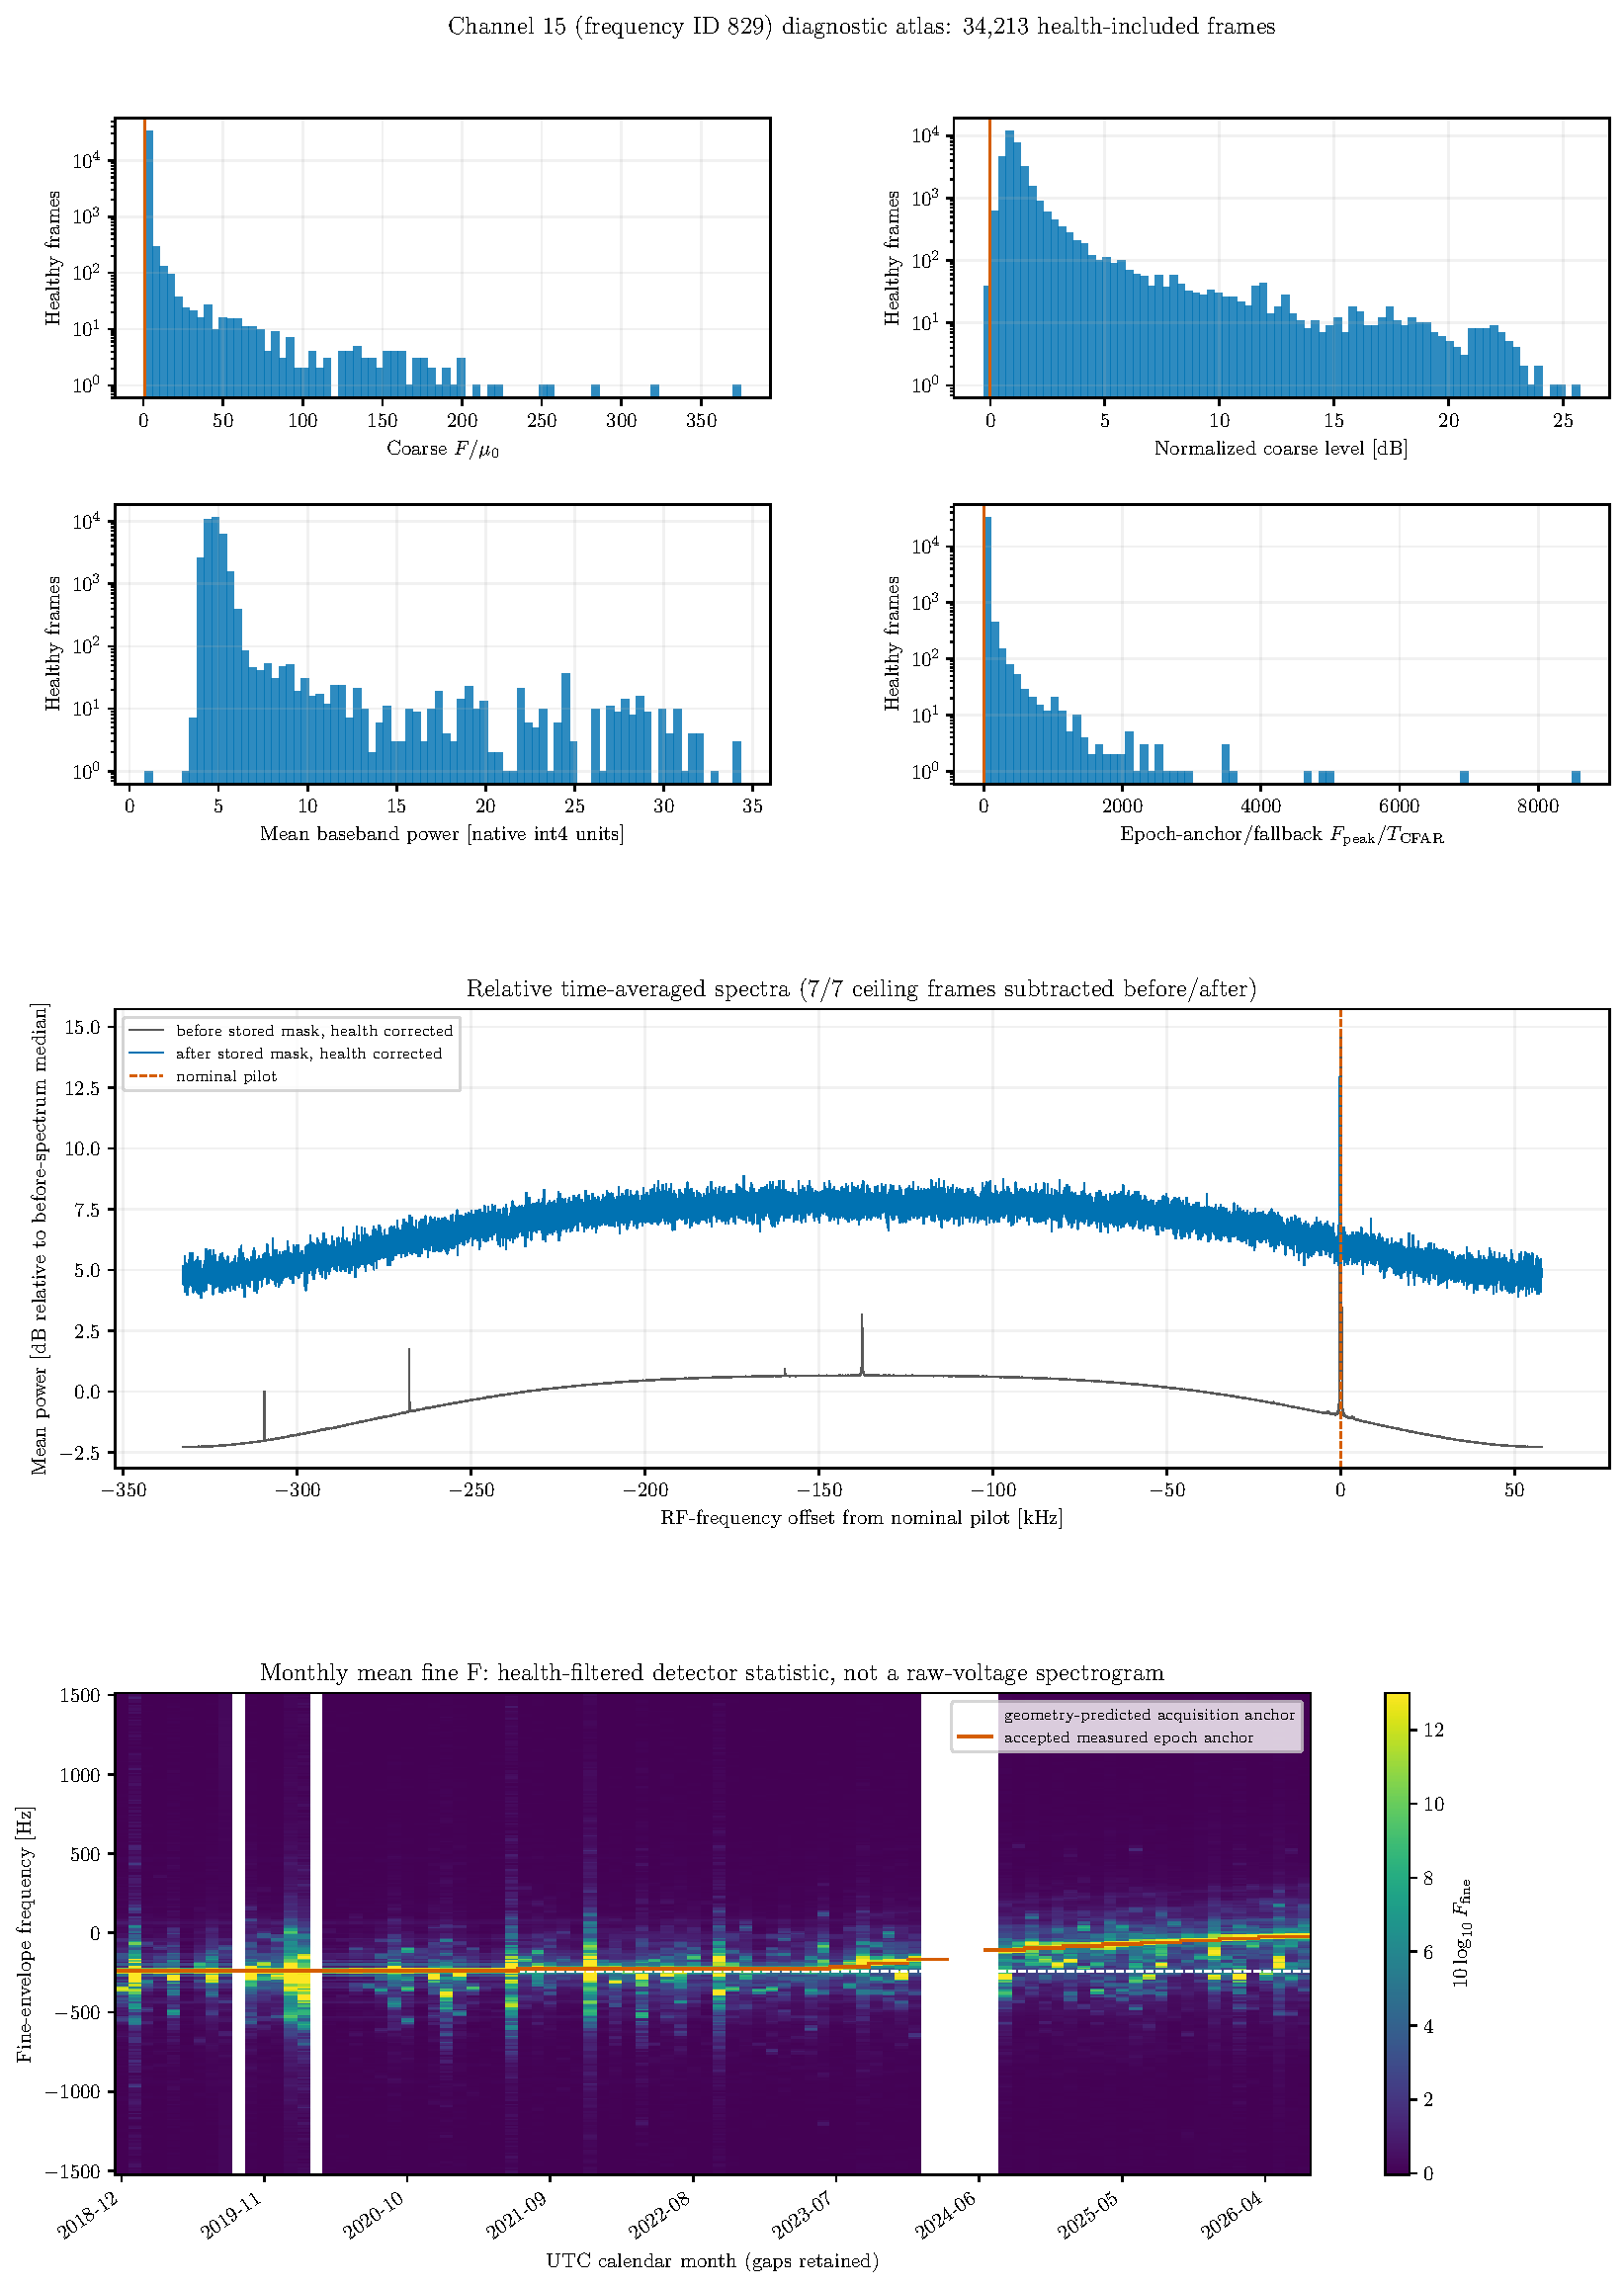
\includegraphics[width=0.98\linewidth,height=0.82\textheight,keepaspectratio]{figs/archive_health_v1/channel_15_diagnostic_atlas.pdf}
\caption{Channel 15 (\texttt{freq\_id}=829) health-filtered archive diagnostics.}
\label{fig:archive:atlas:15}
\end{figure}
\clearpage

\begin{figure}[p]
\centering
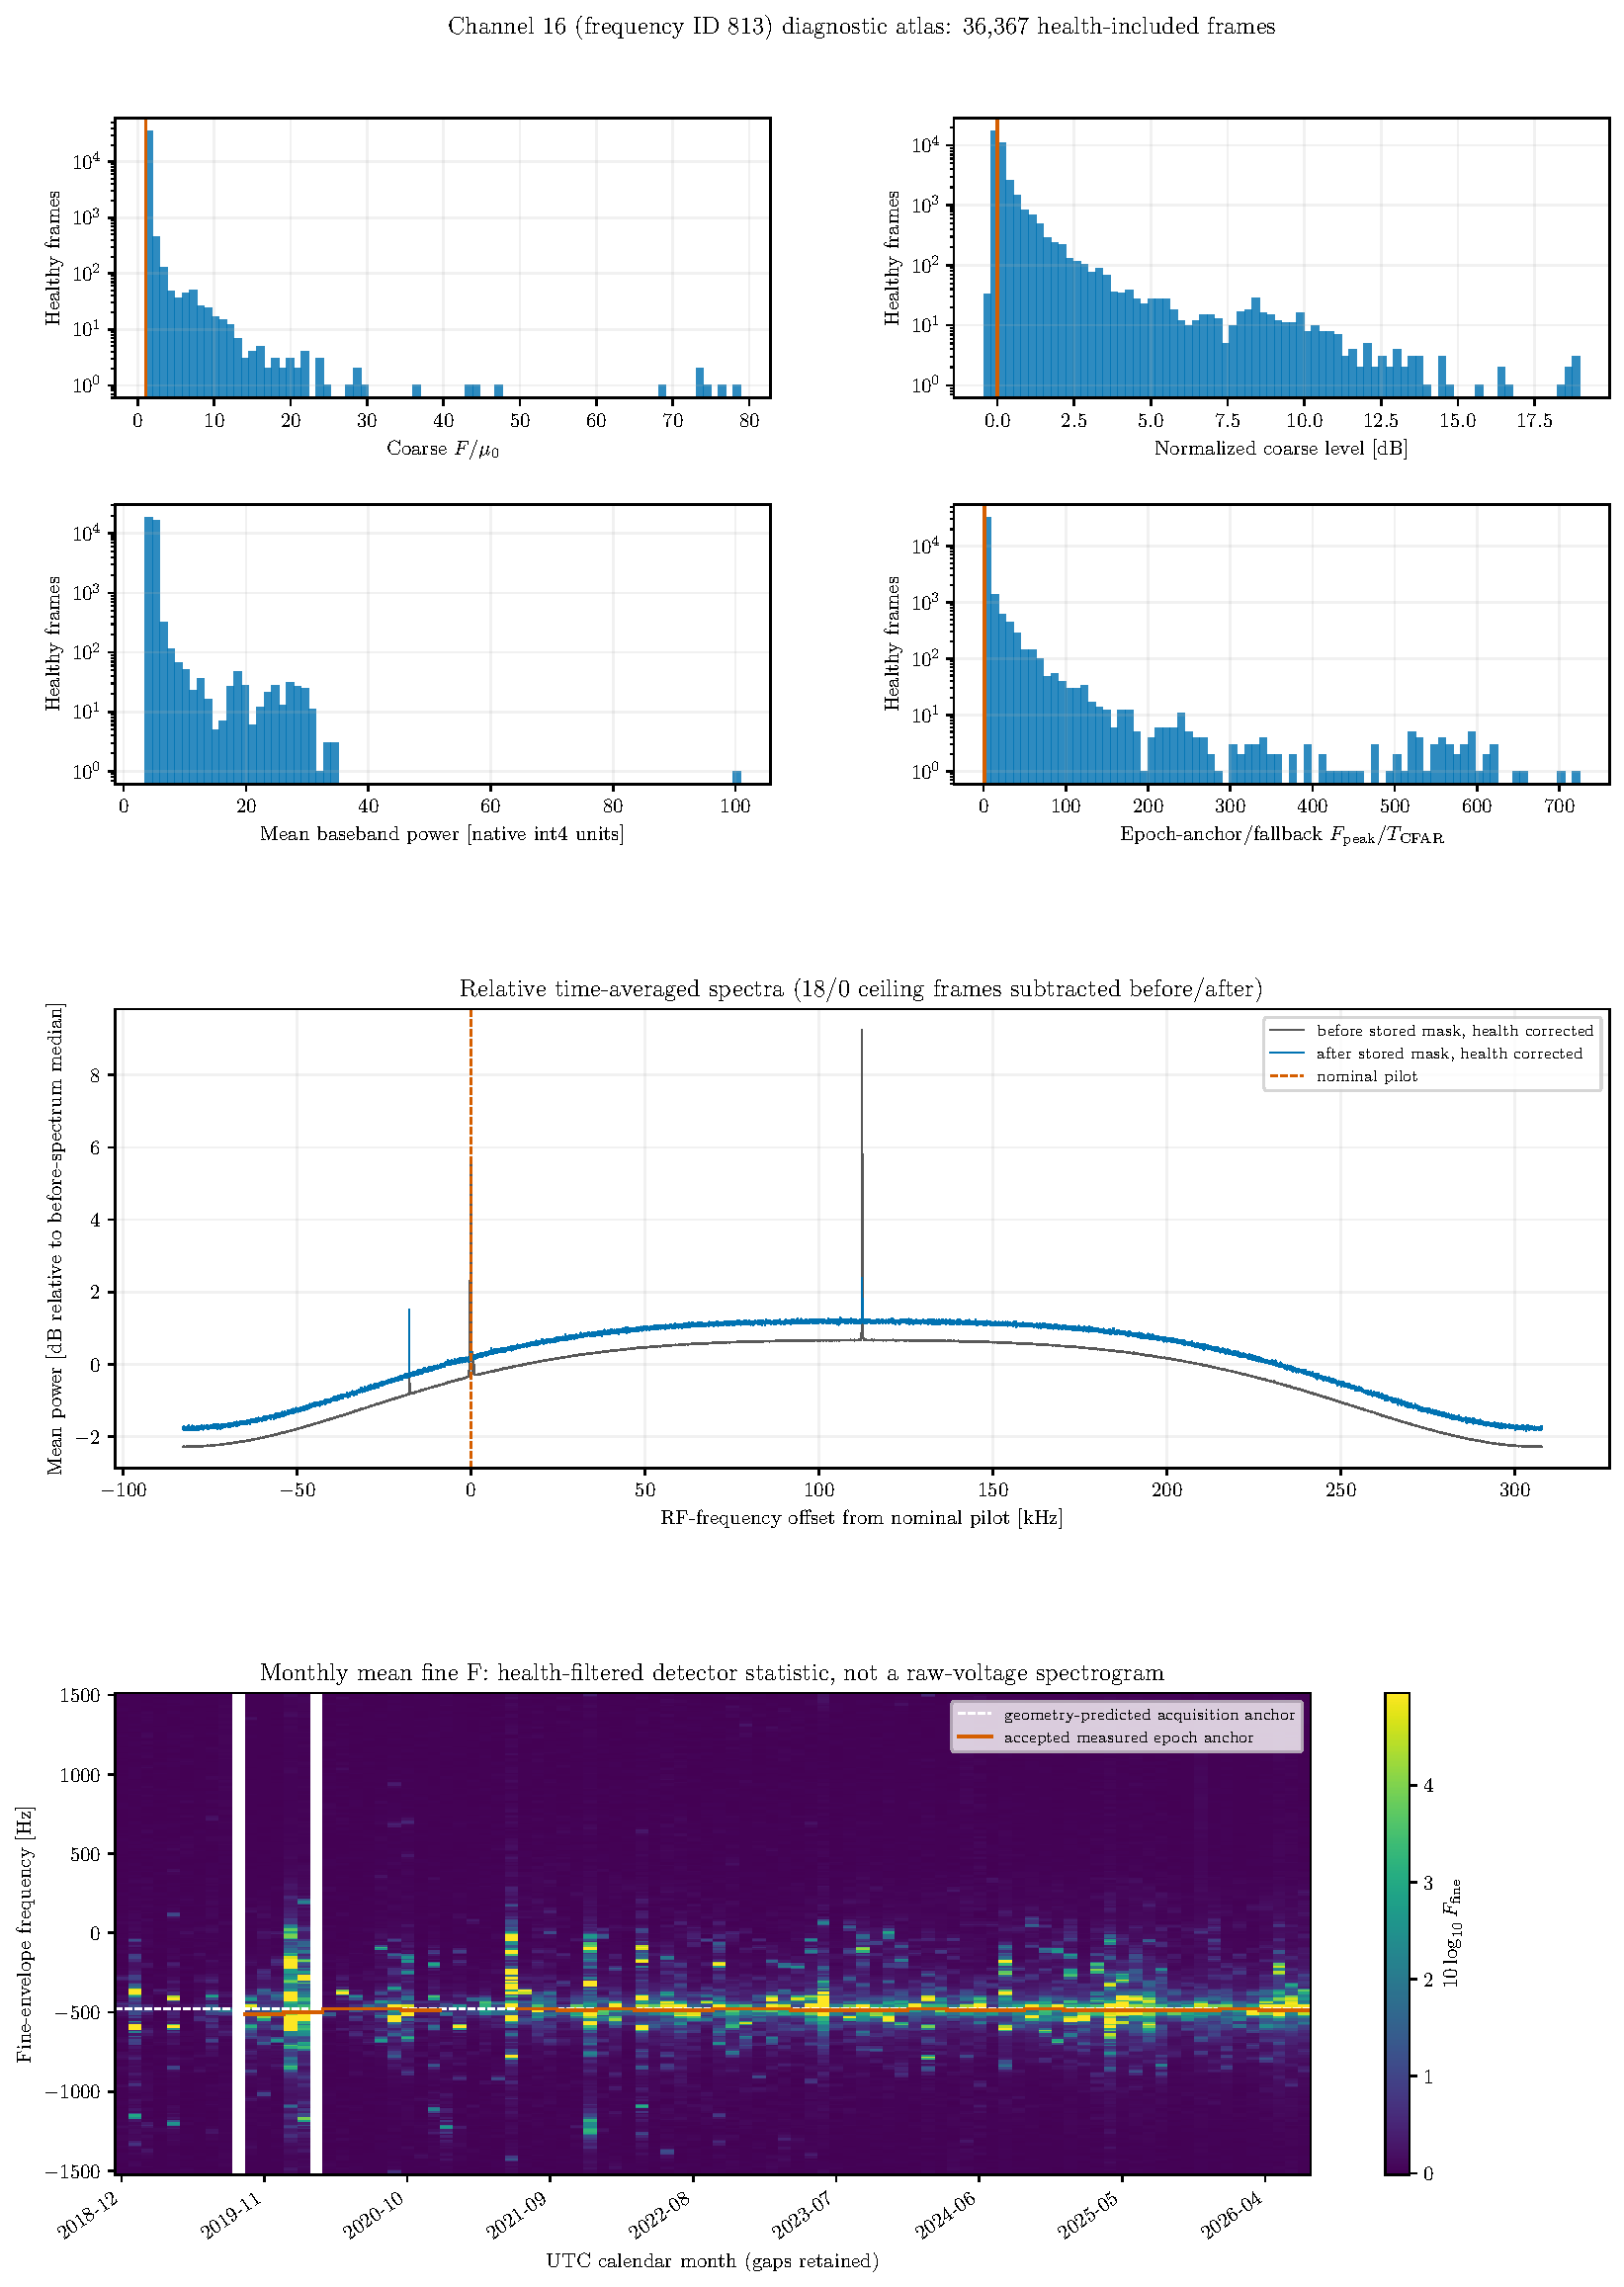
\includegraphics[width=0.98\linewidth,height=0.82\textheight,keepaspectratio]{figs/archive_health_v1/channel_16_diagnostic_atlas.pdf}
\caption{Channel 16 (\texttt{freq\_id}=813) health-filtered archive diagnostics.}
\label{fig:archive:atlas:16}
\end{figure}
\clearpage

\begin{figure}[p]
\centering
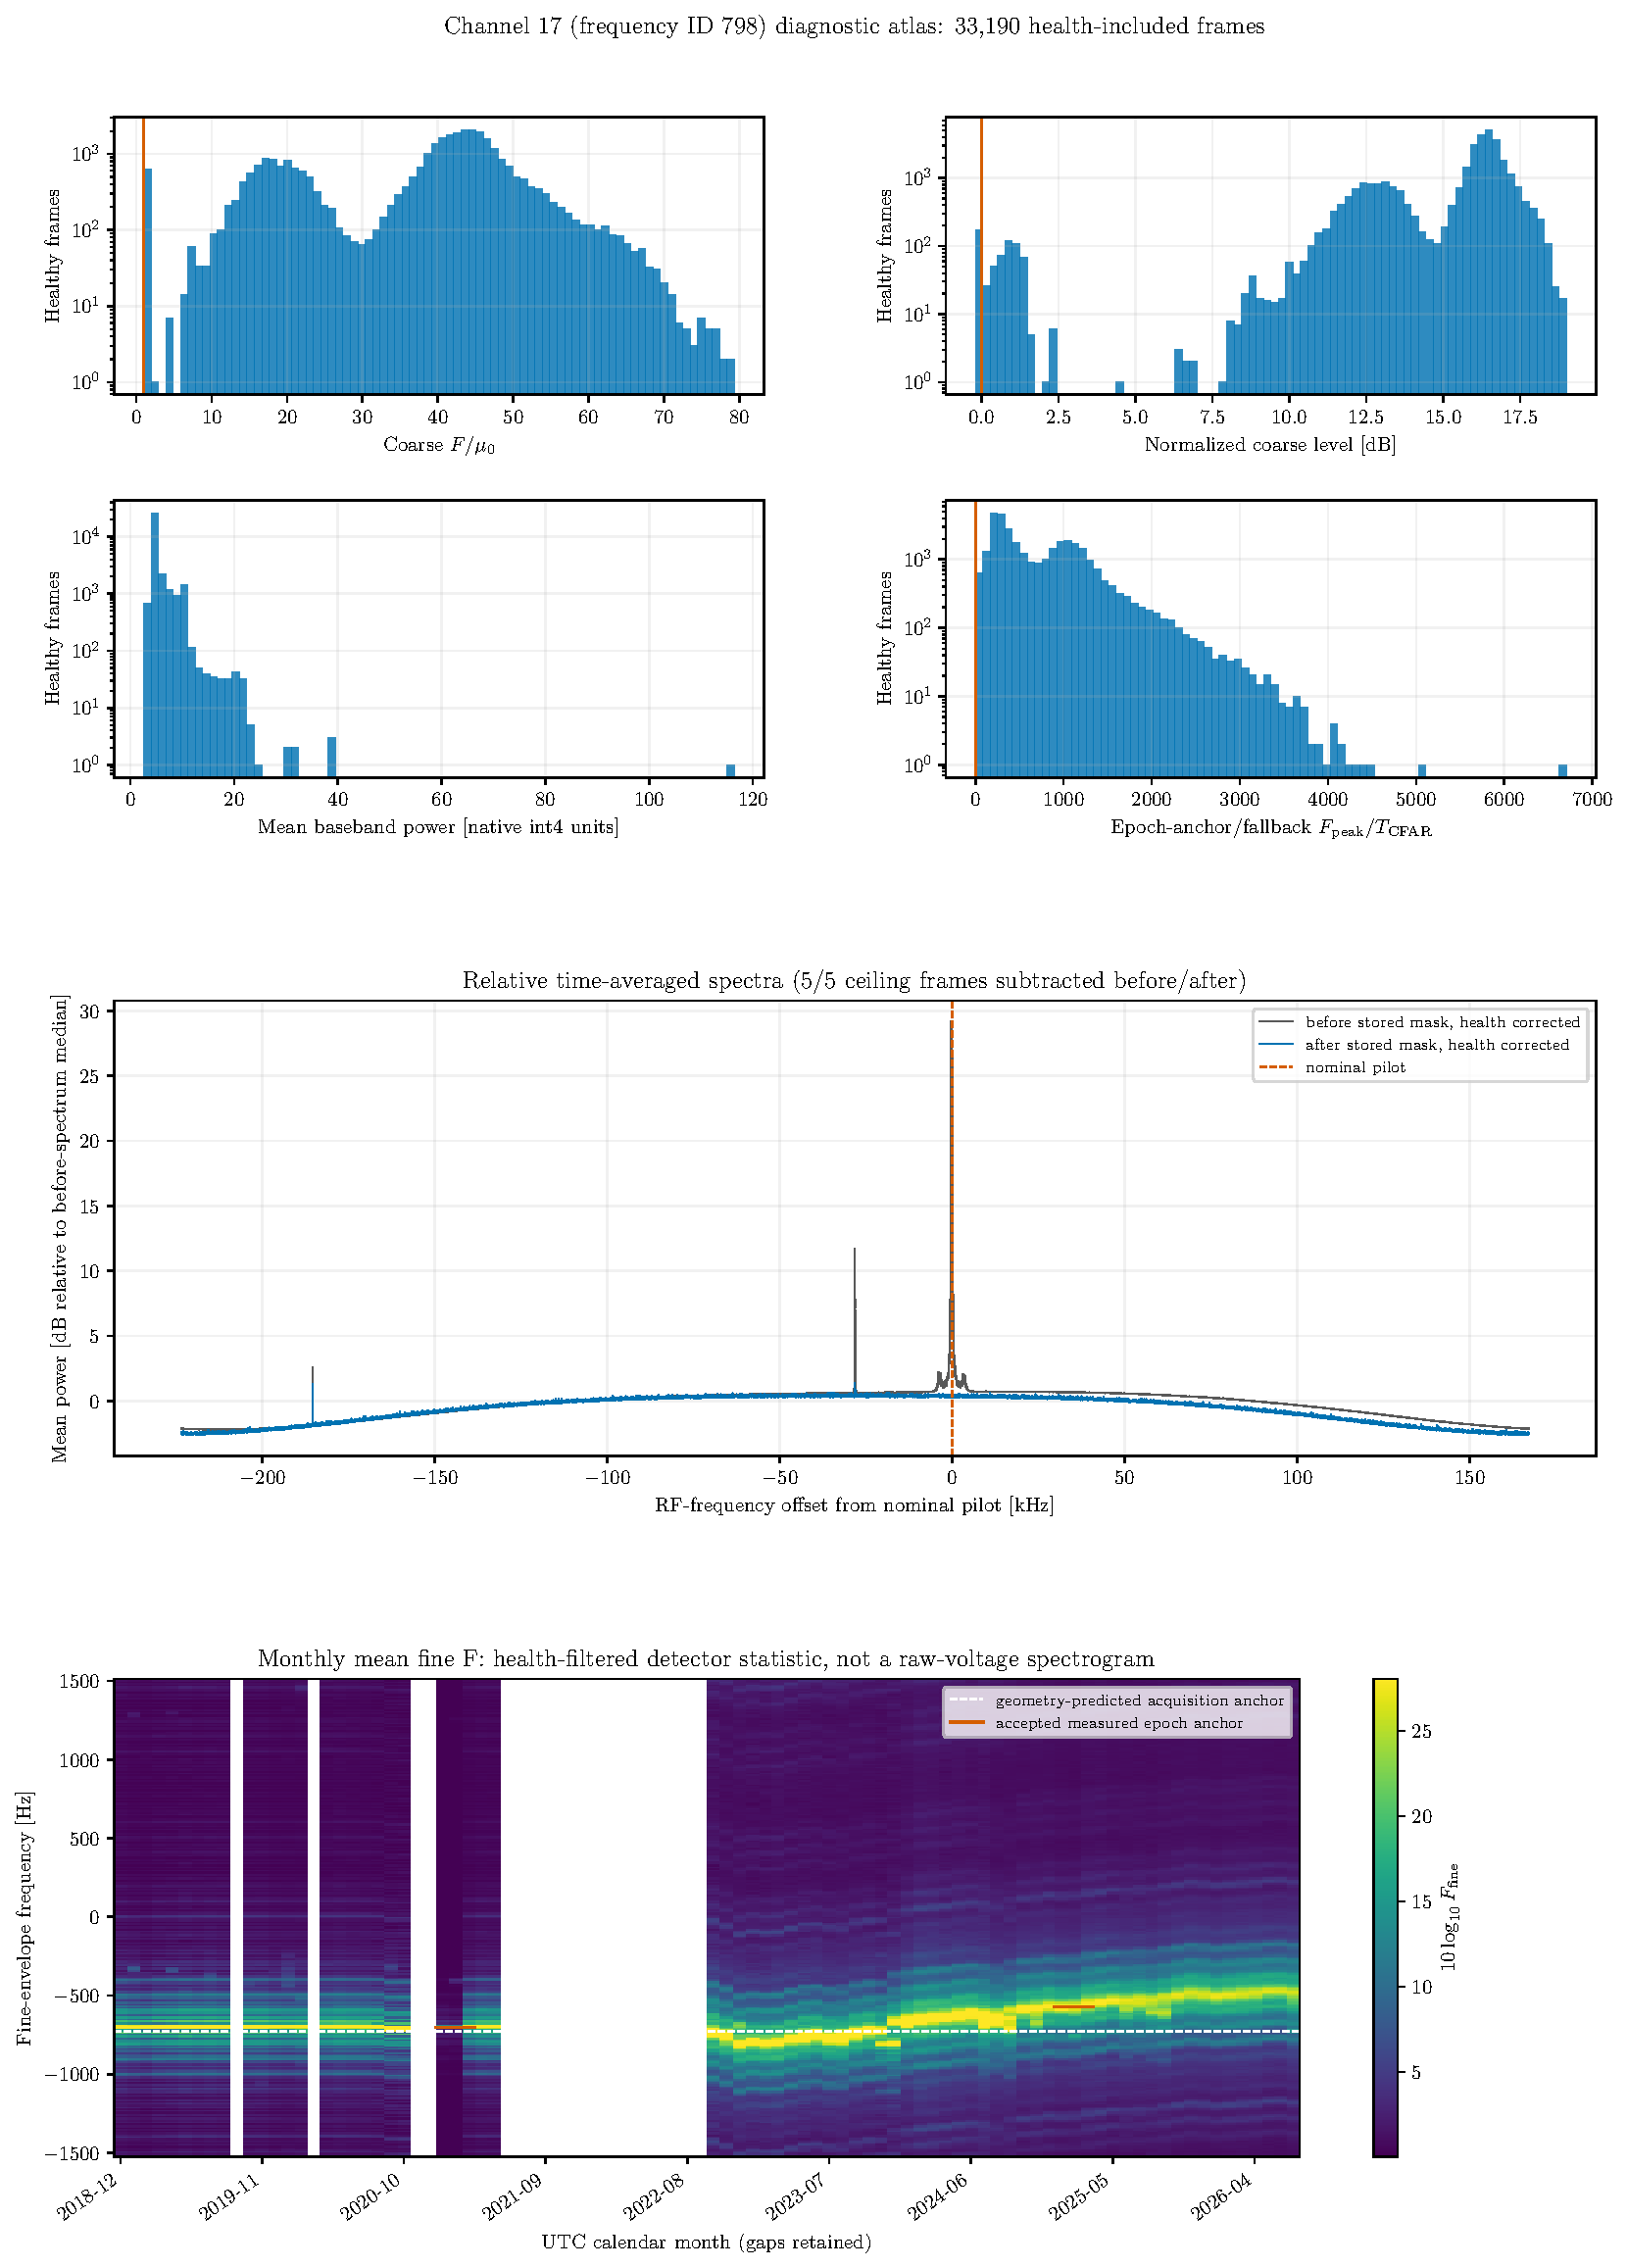
\includegraphics[width=0.98\linewidth,height=0.82\textheight,keepaspectratio]{figs/archive_health_v1/channel_17_diagnostic_atlas.pdf}
\caption{Channel 17 (\texttt{freq\_id}=798).  Its nine excluded rows comprise the four detector-invalid all-zero frames and five constant-ceiling frames.}
\label{fig:archive:atlas:17}
\end{figure}
\clearpage

\begin{figure}[p]
\centering
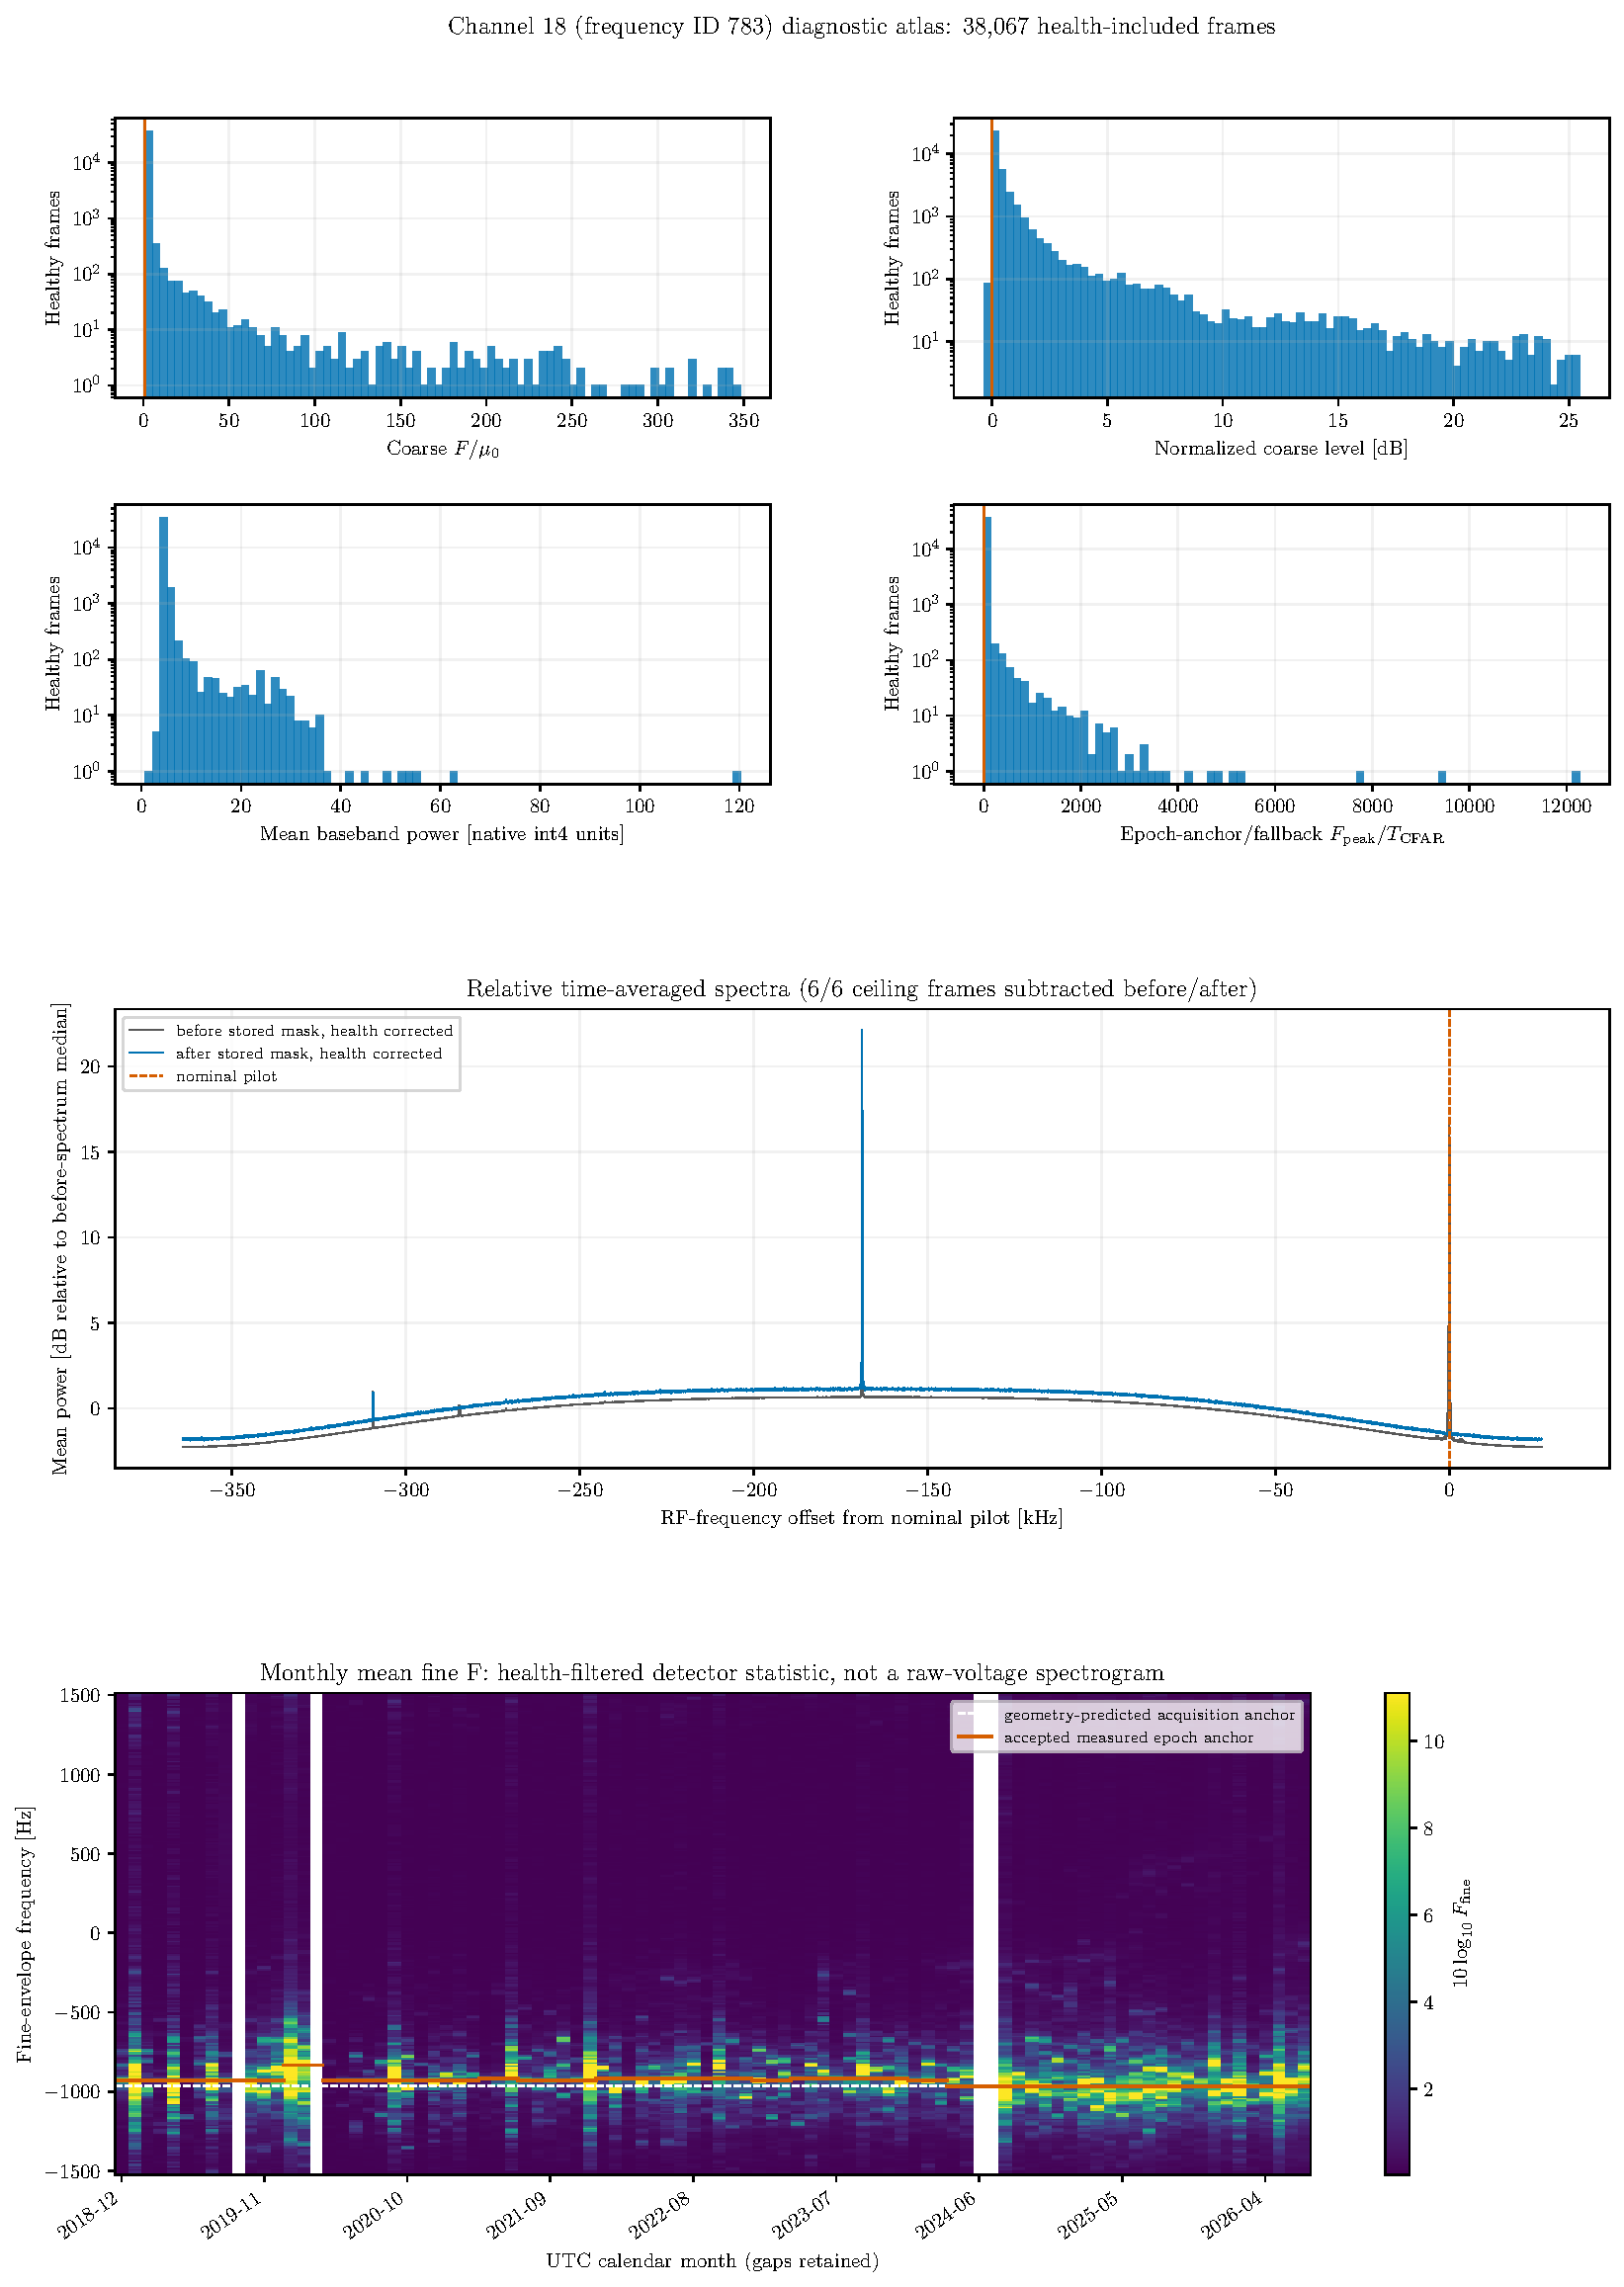
\includegraphics[width=0.98\linewidth,height=0.82\textheight,keepaspectratio]{figs/archive_health_v1/channel_18_diagnostic_atlas.pdf}
\caption{Channel 18 (\texttt{freq\_id}=783) health-filtered archive diagnostics.}
\label{fig:archive:atlas:18}
\end{figure}
\clearpage

\begin{figure}[p]
\centering
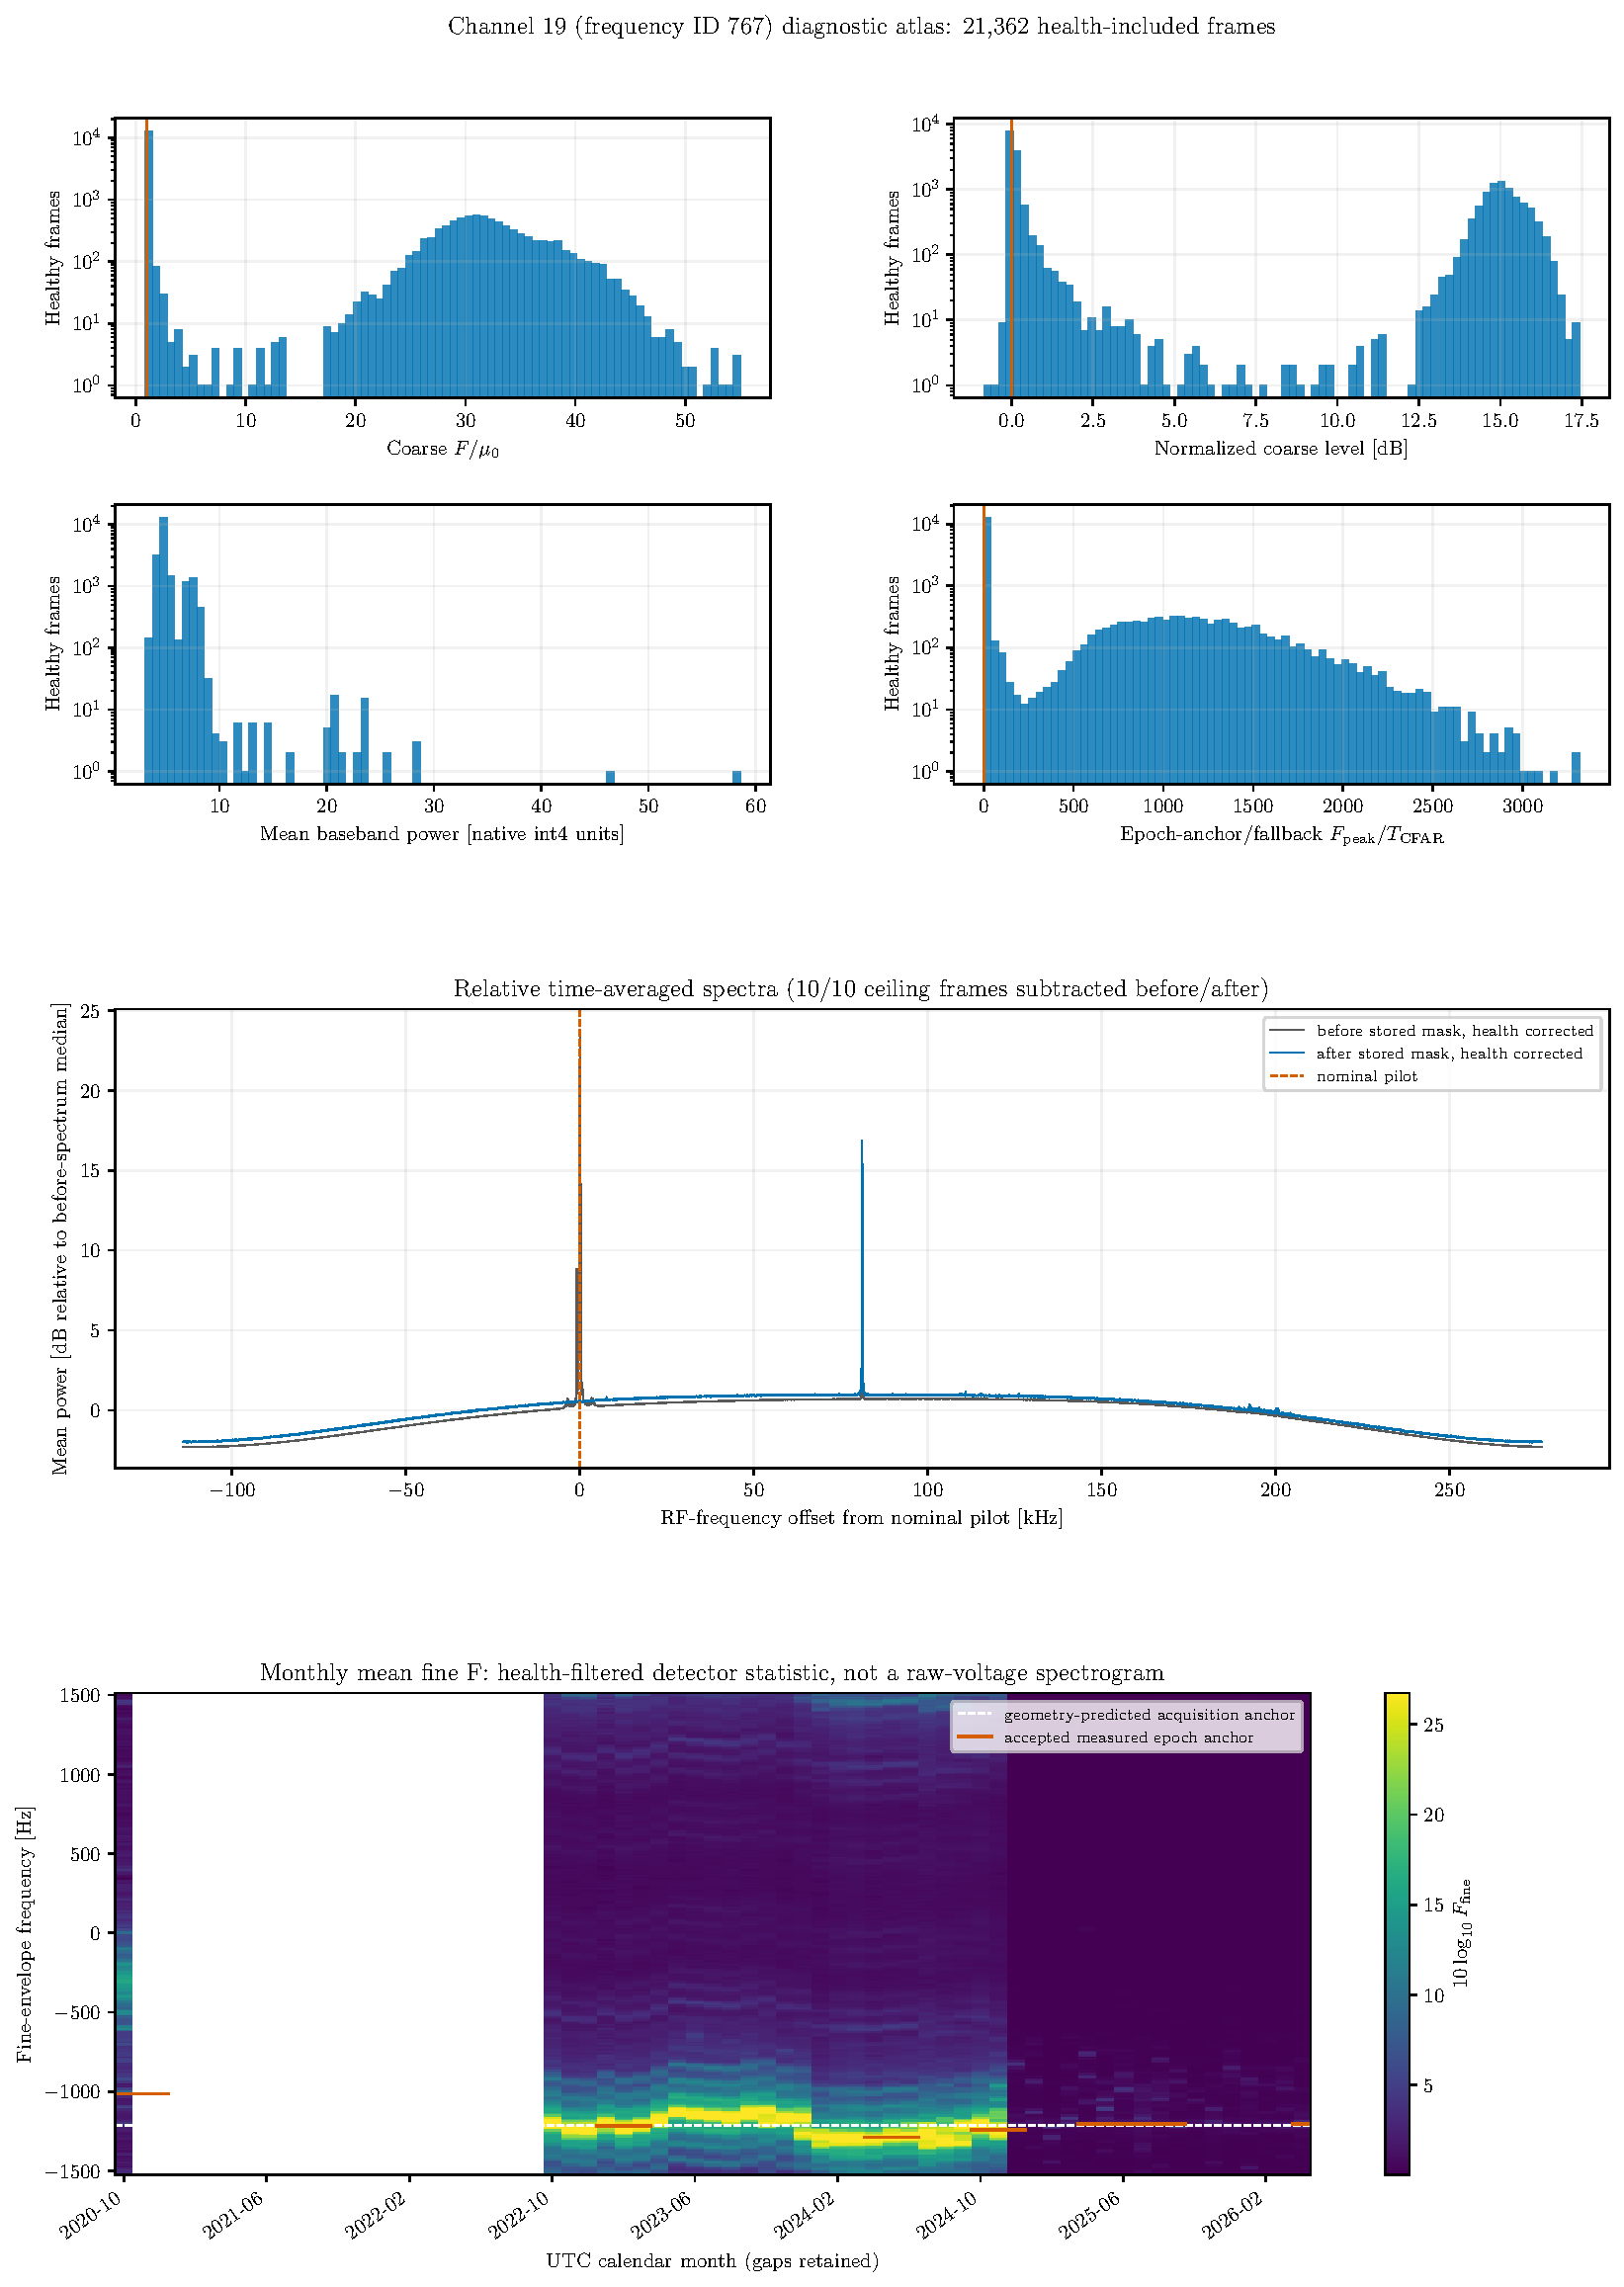
\includegraphics[width=0.98\linewidth,height=0.82\textheight,keepaspectratio]{figs/archive_health_v1/channel_19_diagnostic_atlas.pdf}
\caption{Channel 19 (\texttt{freq\_id}=767) health-filtered archive diagnostics.}
\label{fig:archive:atlas:19}
\end{figure}
\clearpage

\begin{figure}[p]
\centering
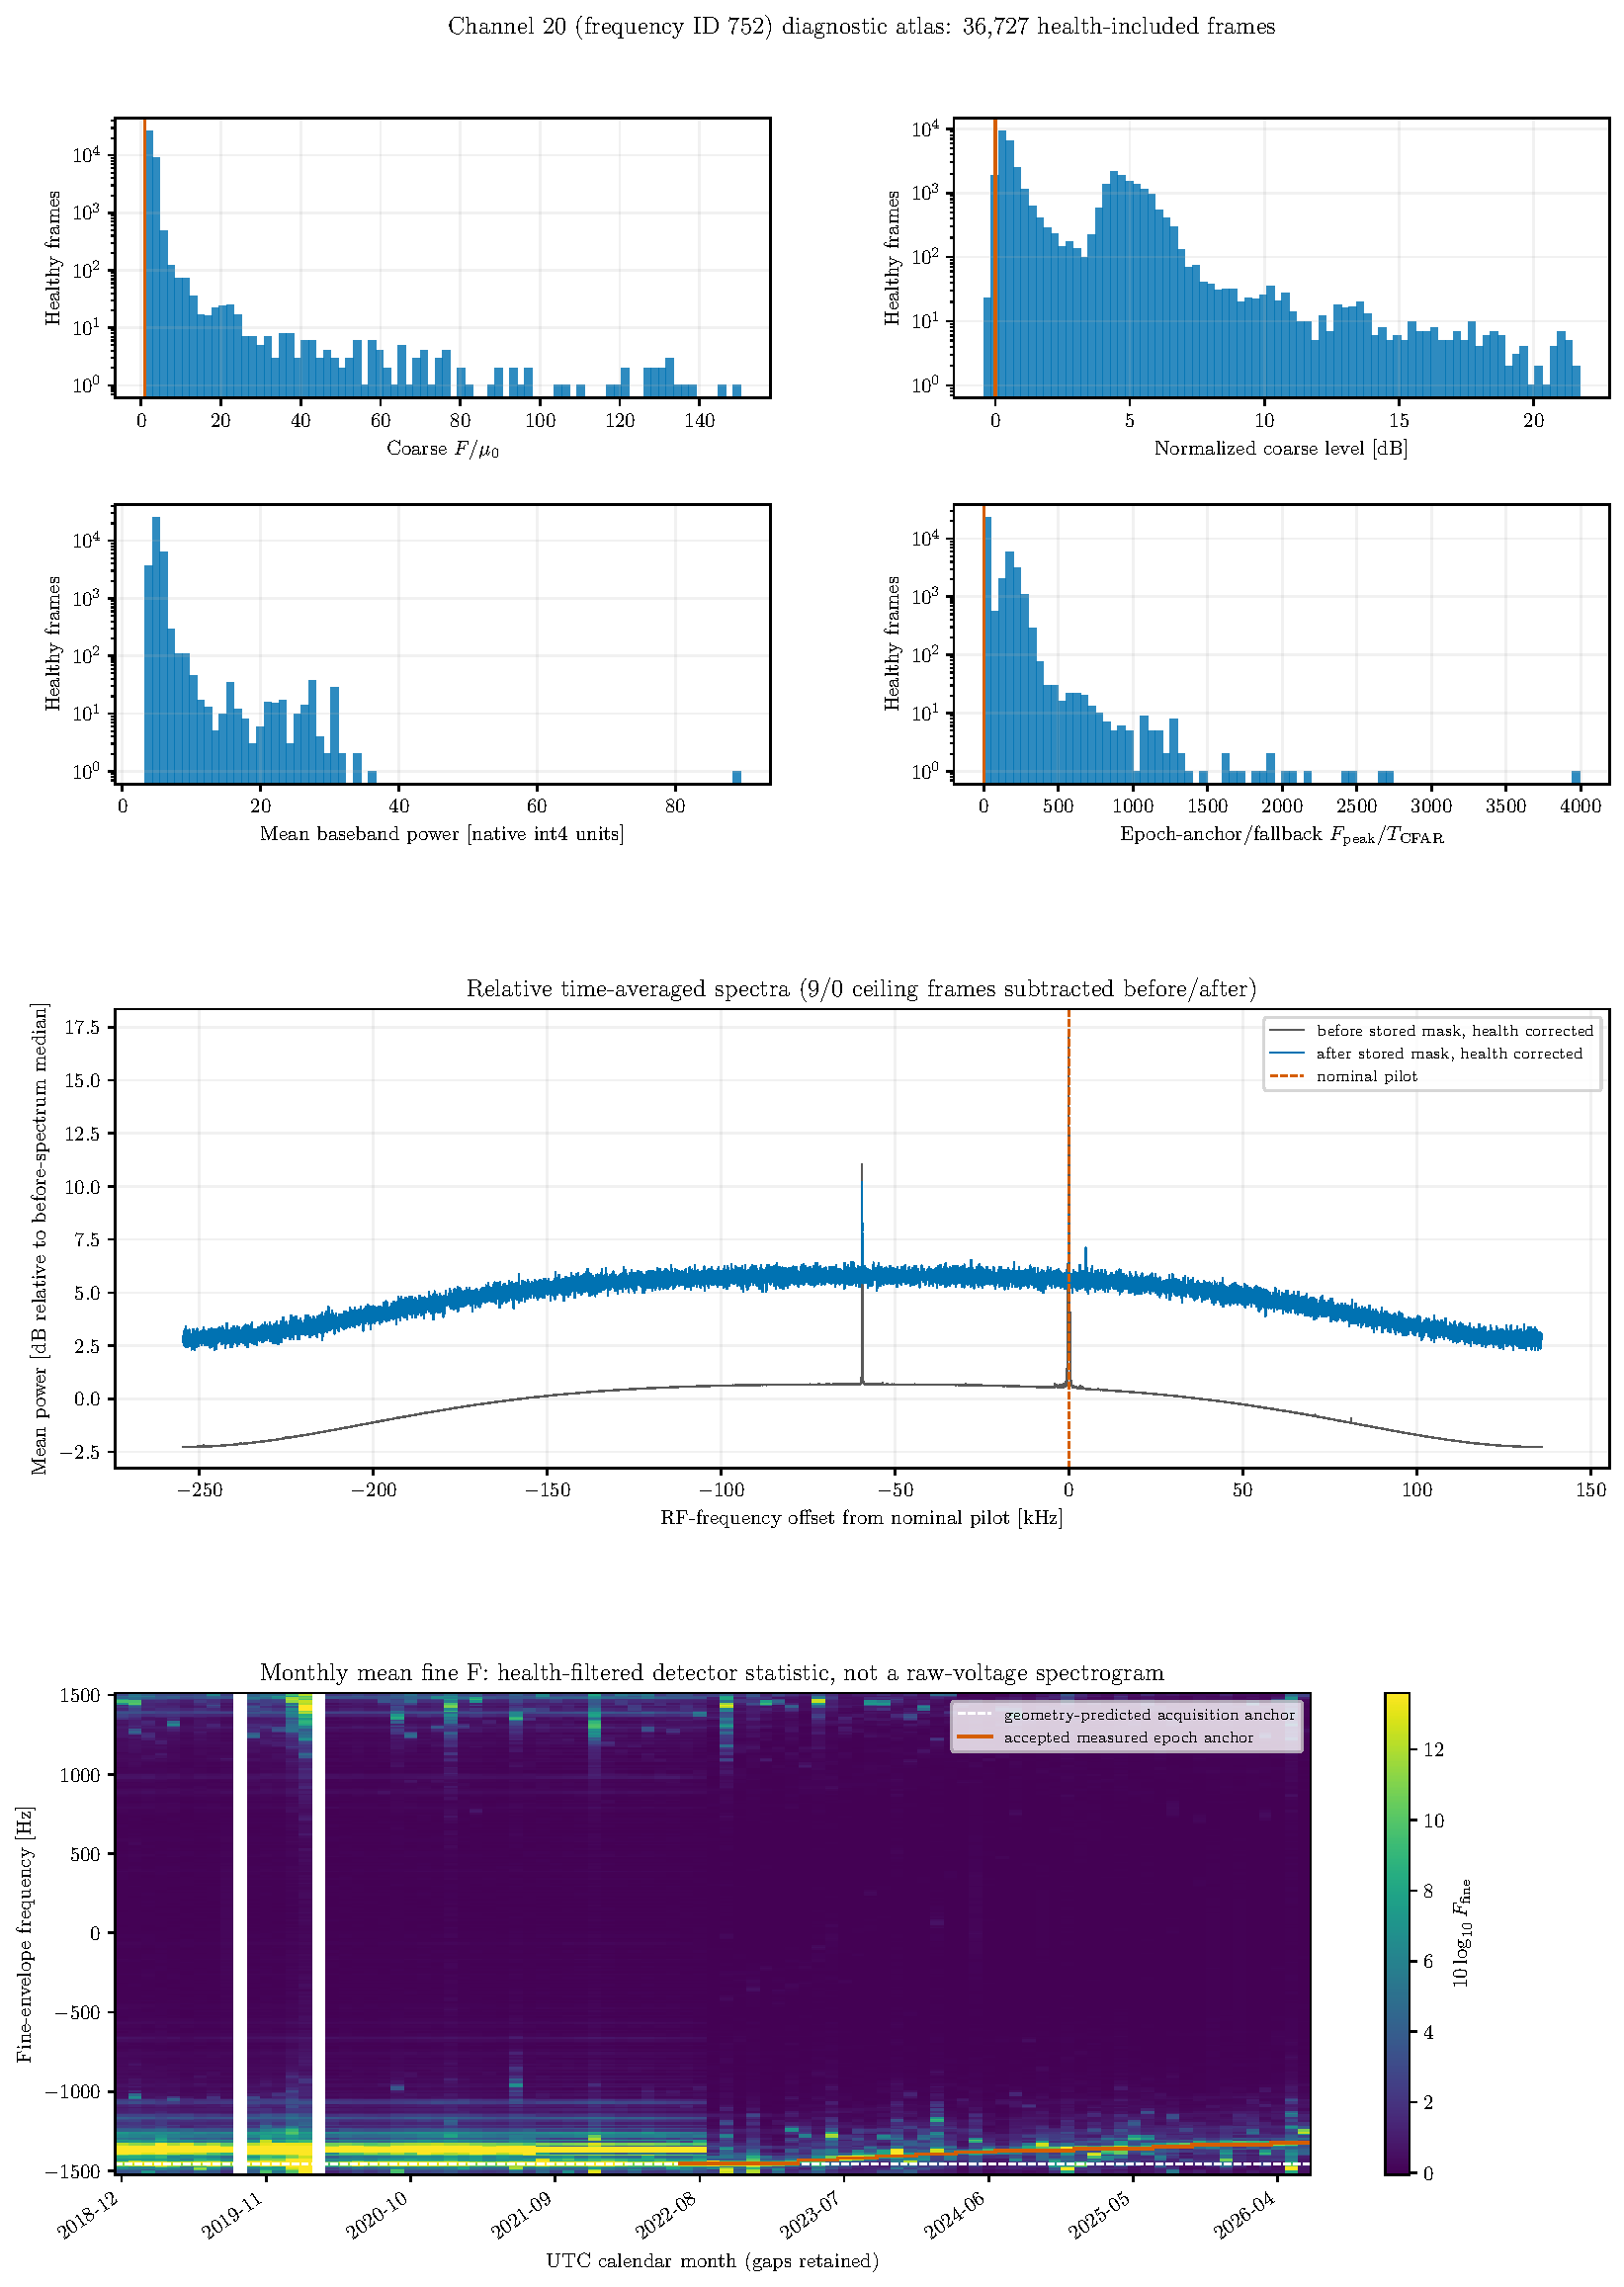
\includegraphics[width=0.98\linewidth,height=0.82\textheight,keepaspectratio]{figs/archive_health_v1/channel_20_diagnostic_atlas.pdf}
\caption{Channel 20 (\texttt{freq\_id}=752) health-filtered archive diagnostics.}
\label{fig:archive:atlas:20}
\end{figure}
\clearpage

\begin{figure}[p]
\centering
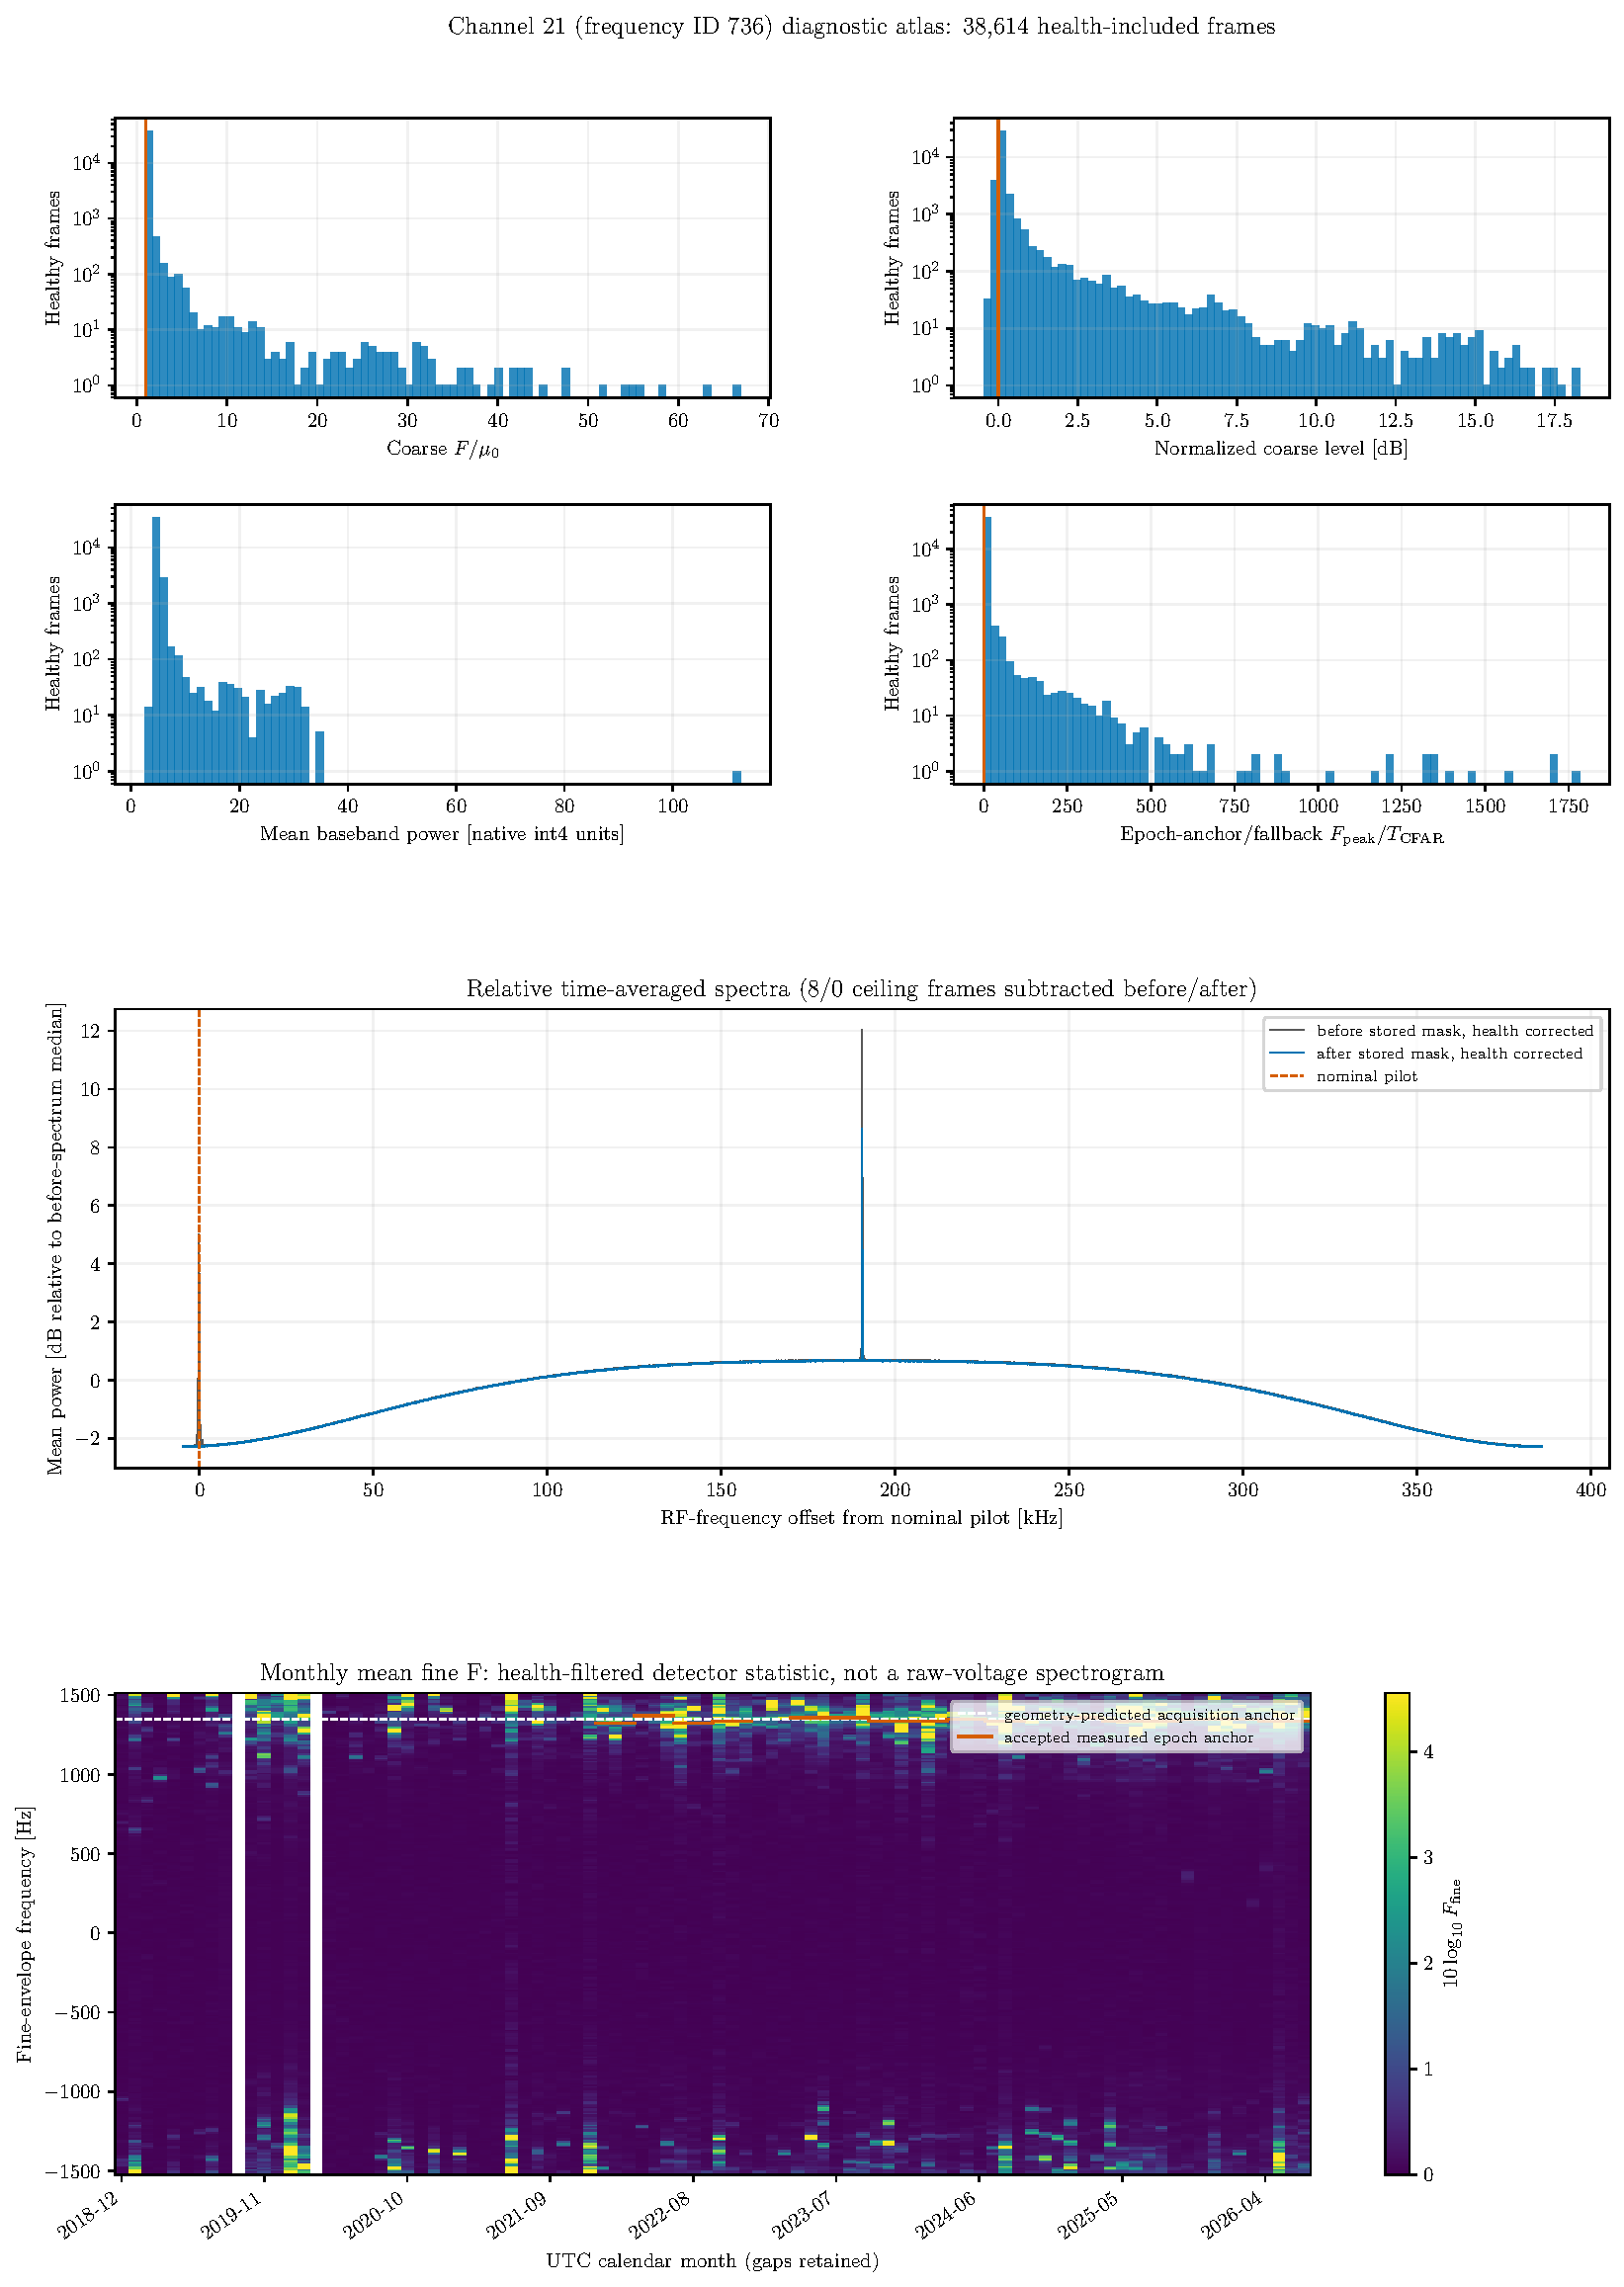
\includegraphics[width=0.98\linewidth,height=0.82\textheight,keepaspectratio]{figs/archive_health_v1/channel_21_diagnostic_atlas.pdf}
\caption{Channel 21 (\texttt{freq\_id}=736) health-filtered archive diagnostics.}
\label{fig:archive:atlas:21}
\end{figure}
\clearpage

\begin{figure}[p]
\centering
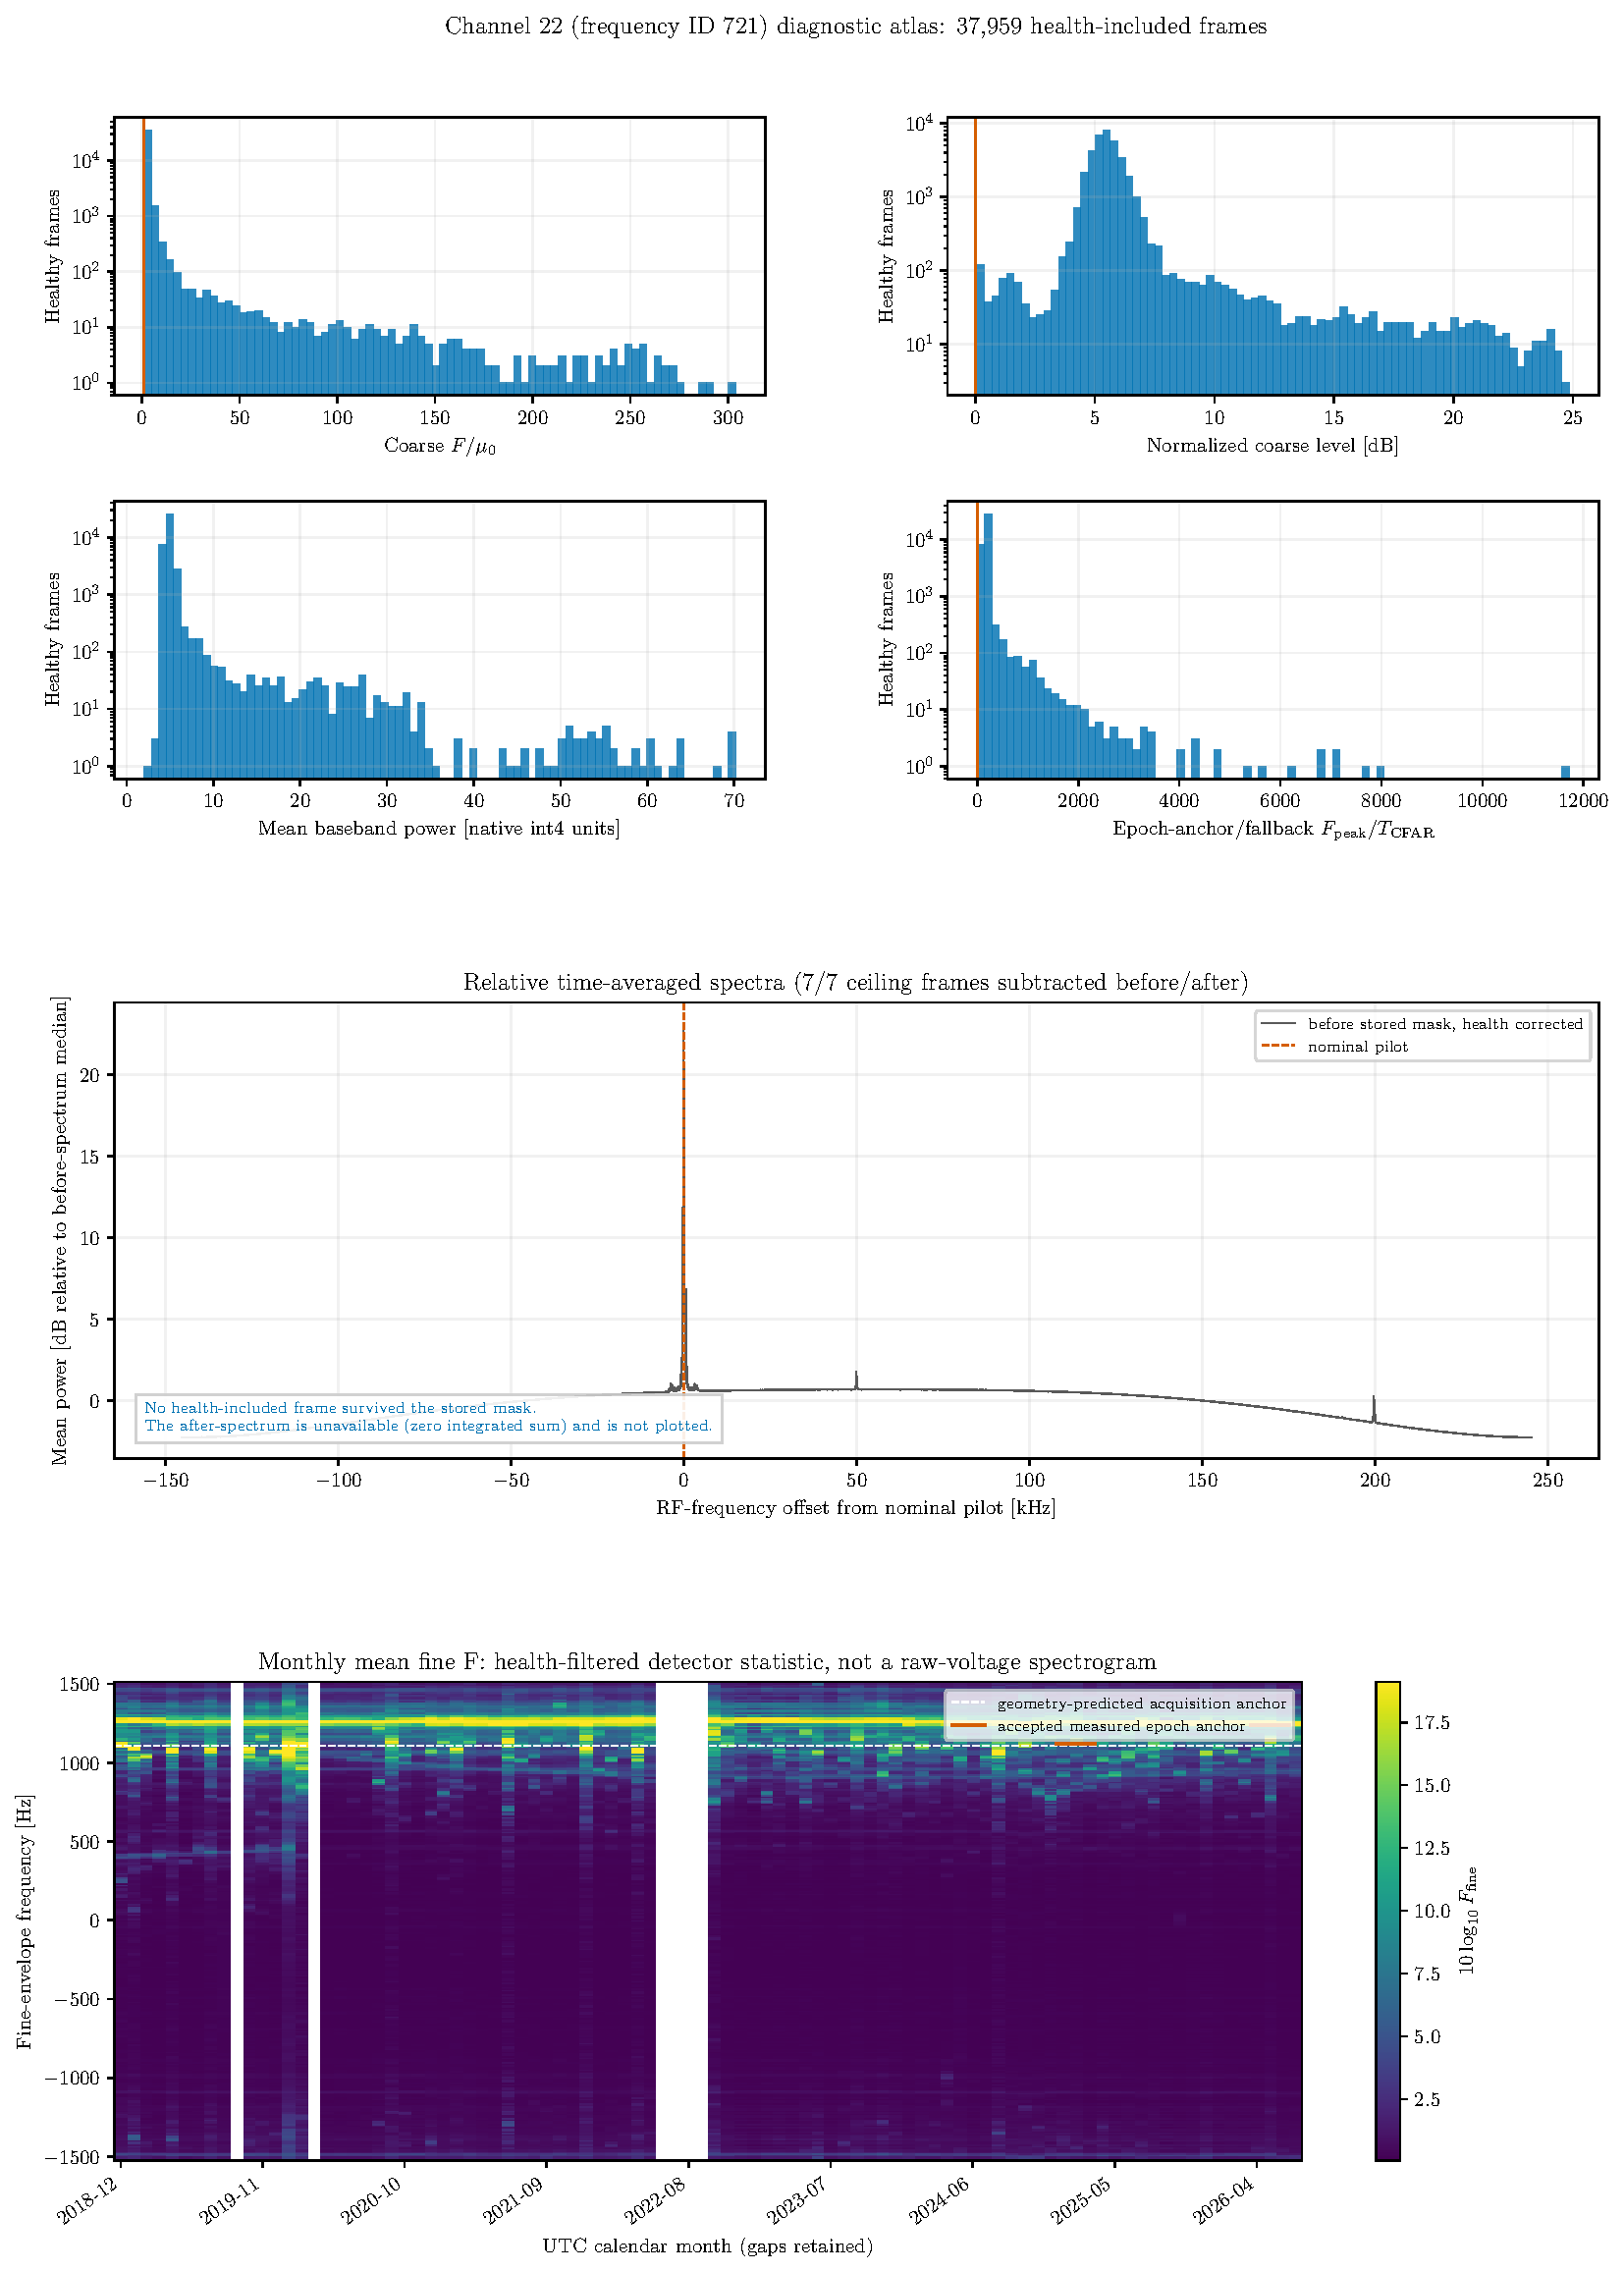
\includegraphics[width=0.98\linewidth,height=0.82\textheight,keepaspectratio]{figs/archive_health_v1/channel_22_diagnostic_atlas.pdf}
\caption{Channel 22 (\texttt{freq\_id}=721).  No health-included frame survives the stored coarse mask, so the after-mask spectrum and empirical residual floor are unavailable.}
\label{fig:archive:atlas:22}
\end{figure}
\clearpage

\begin{figure}[p]
\centering
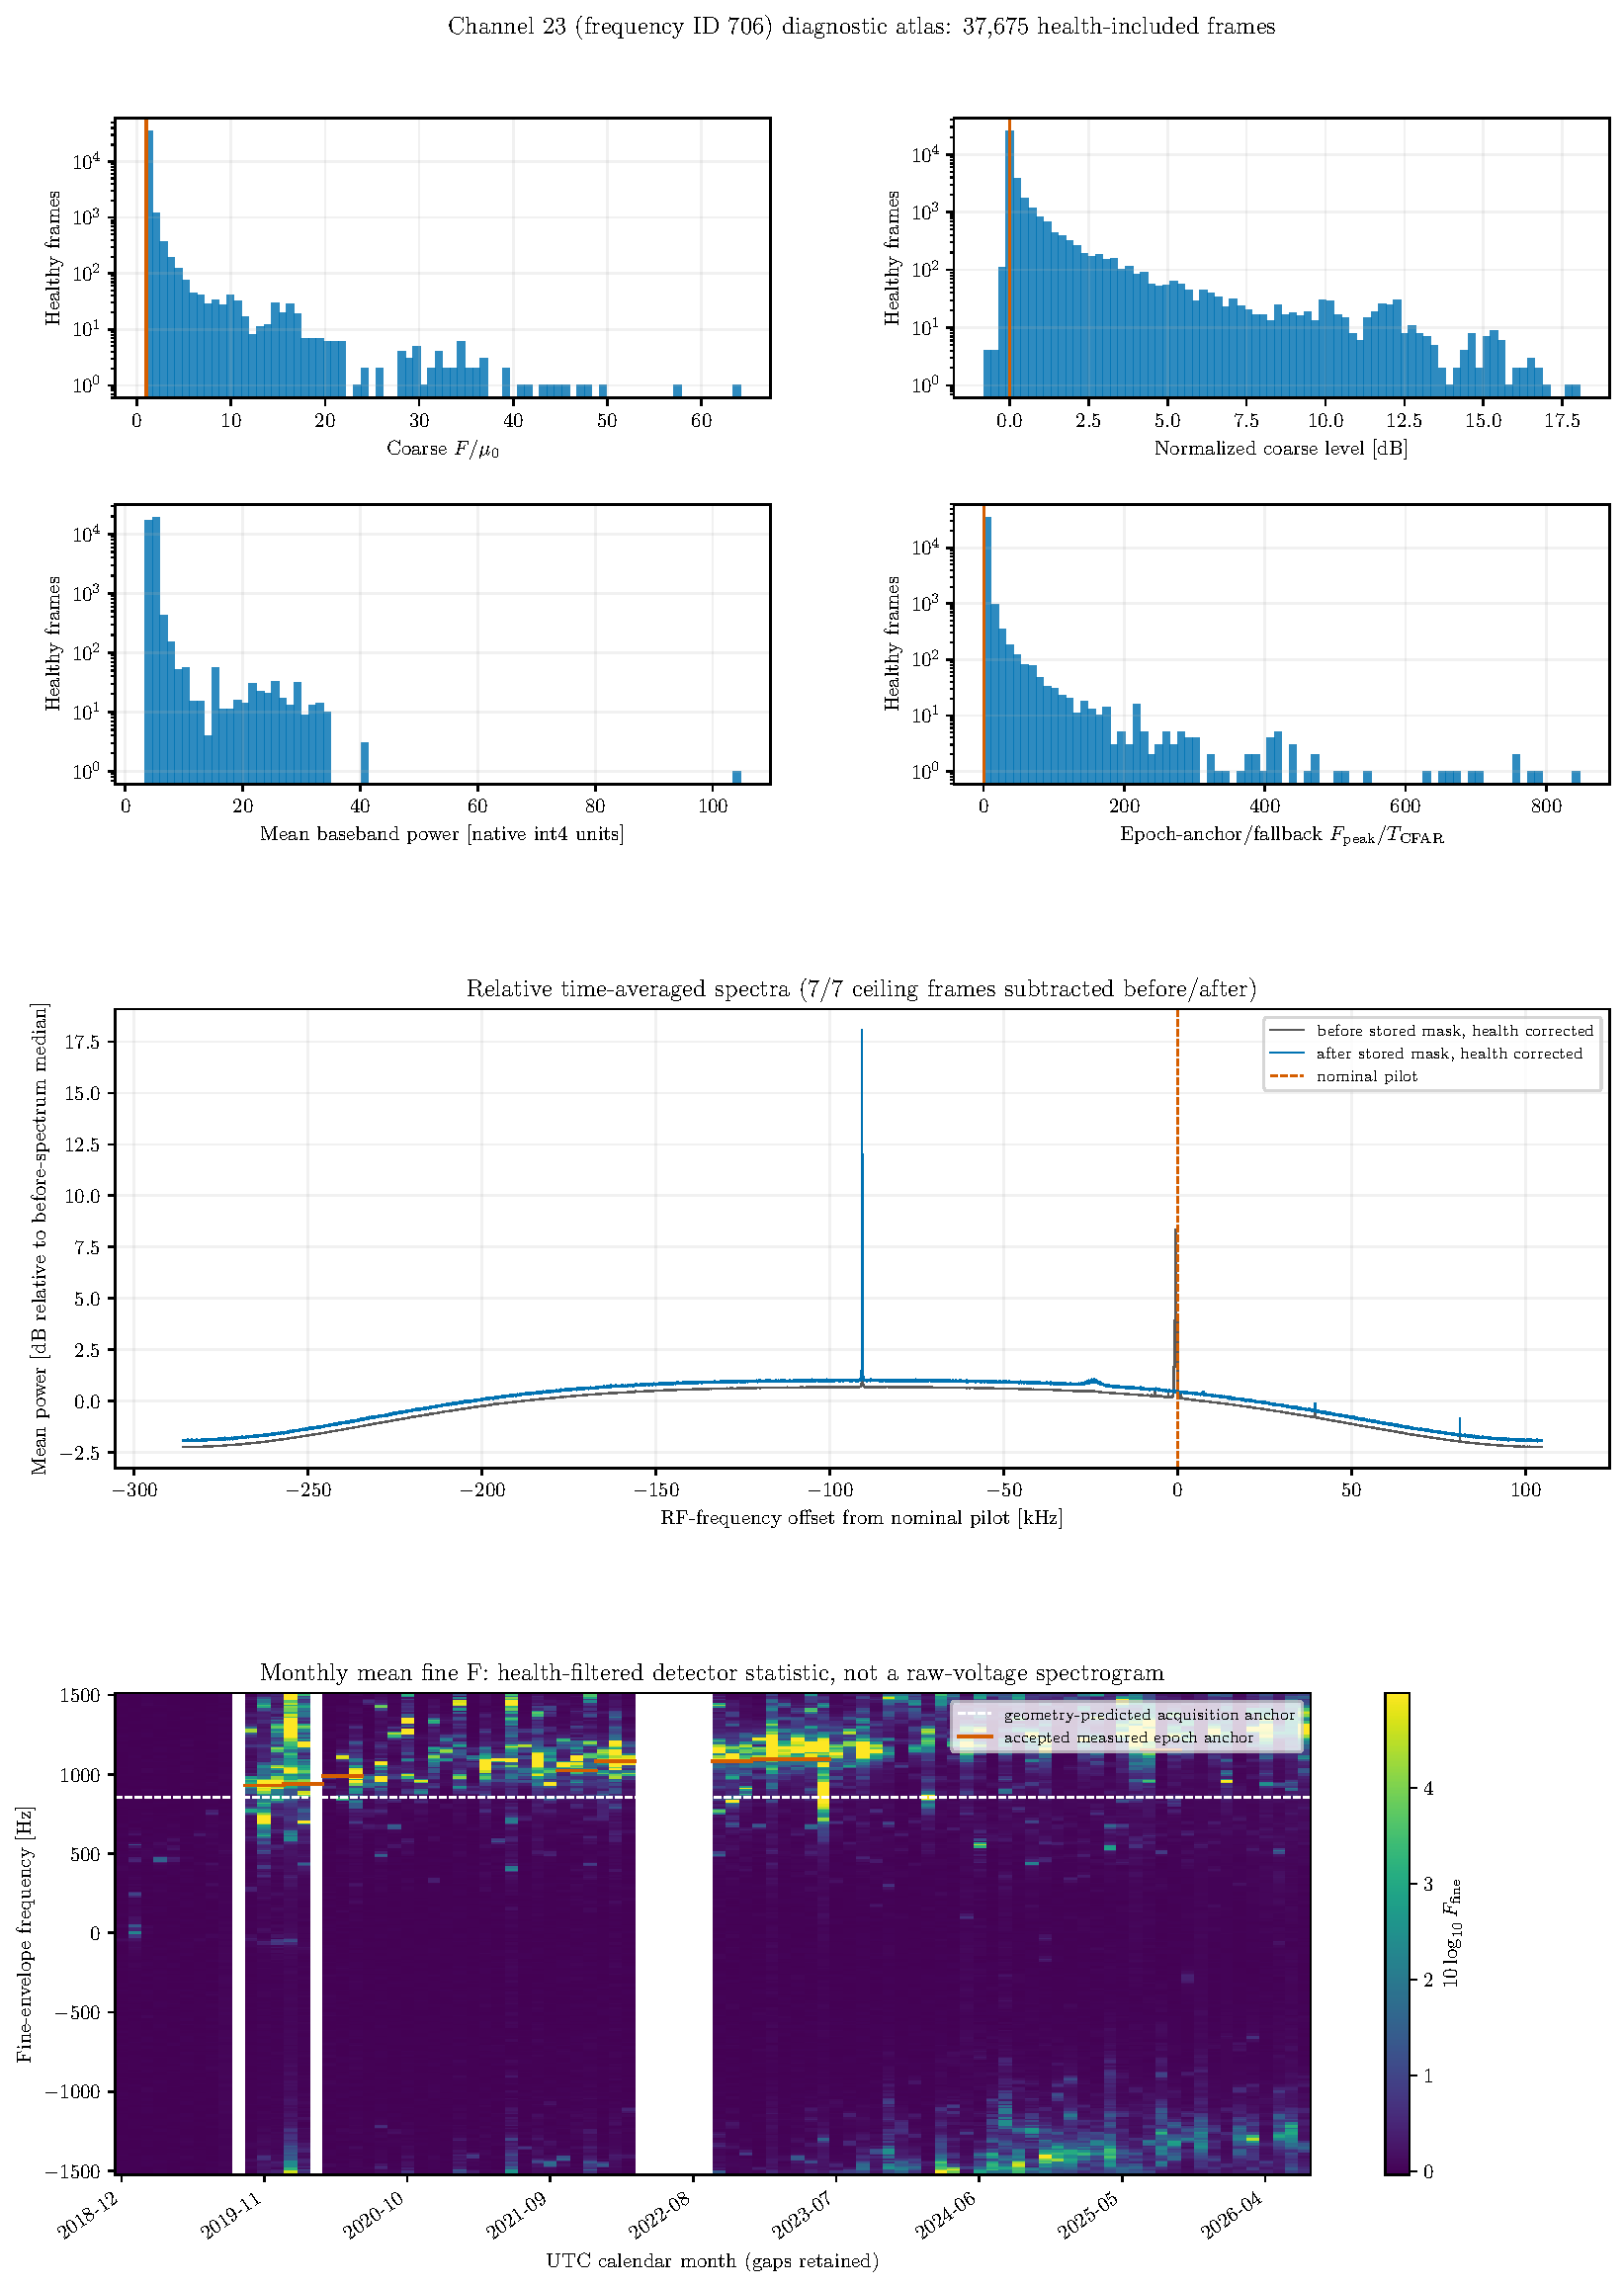
\includegraphics[width=0.98\linewidth,height=0.82\textheight,keepaspectratio]{figs/archive_health_v1/channel_23_diagnostic_atlas.pdf}
\caption{Channel 23 (\texttt{freq\_id}=706) health-filtered archive diagnostics.}
\label{fig:archive:atlas:23}
\end{figure}
\clearpage

\begin{figure}[p]
\centering
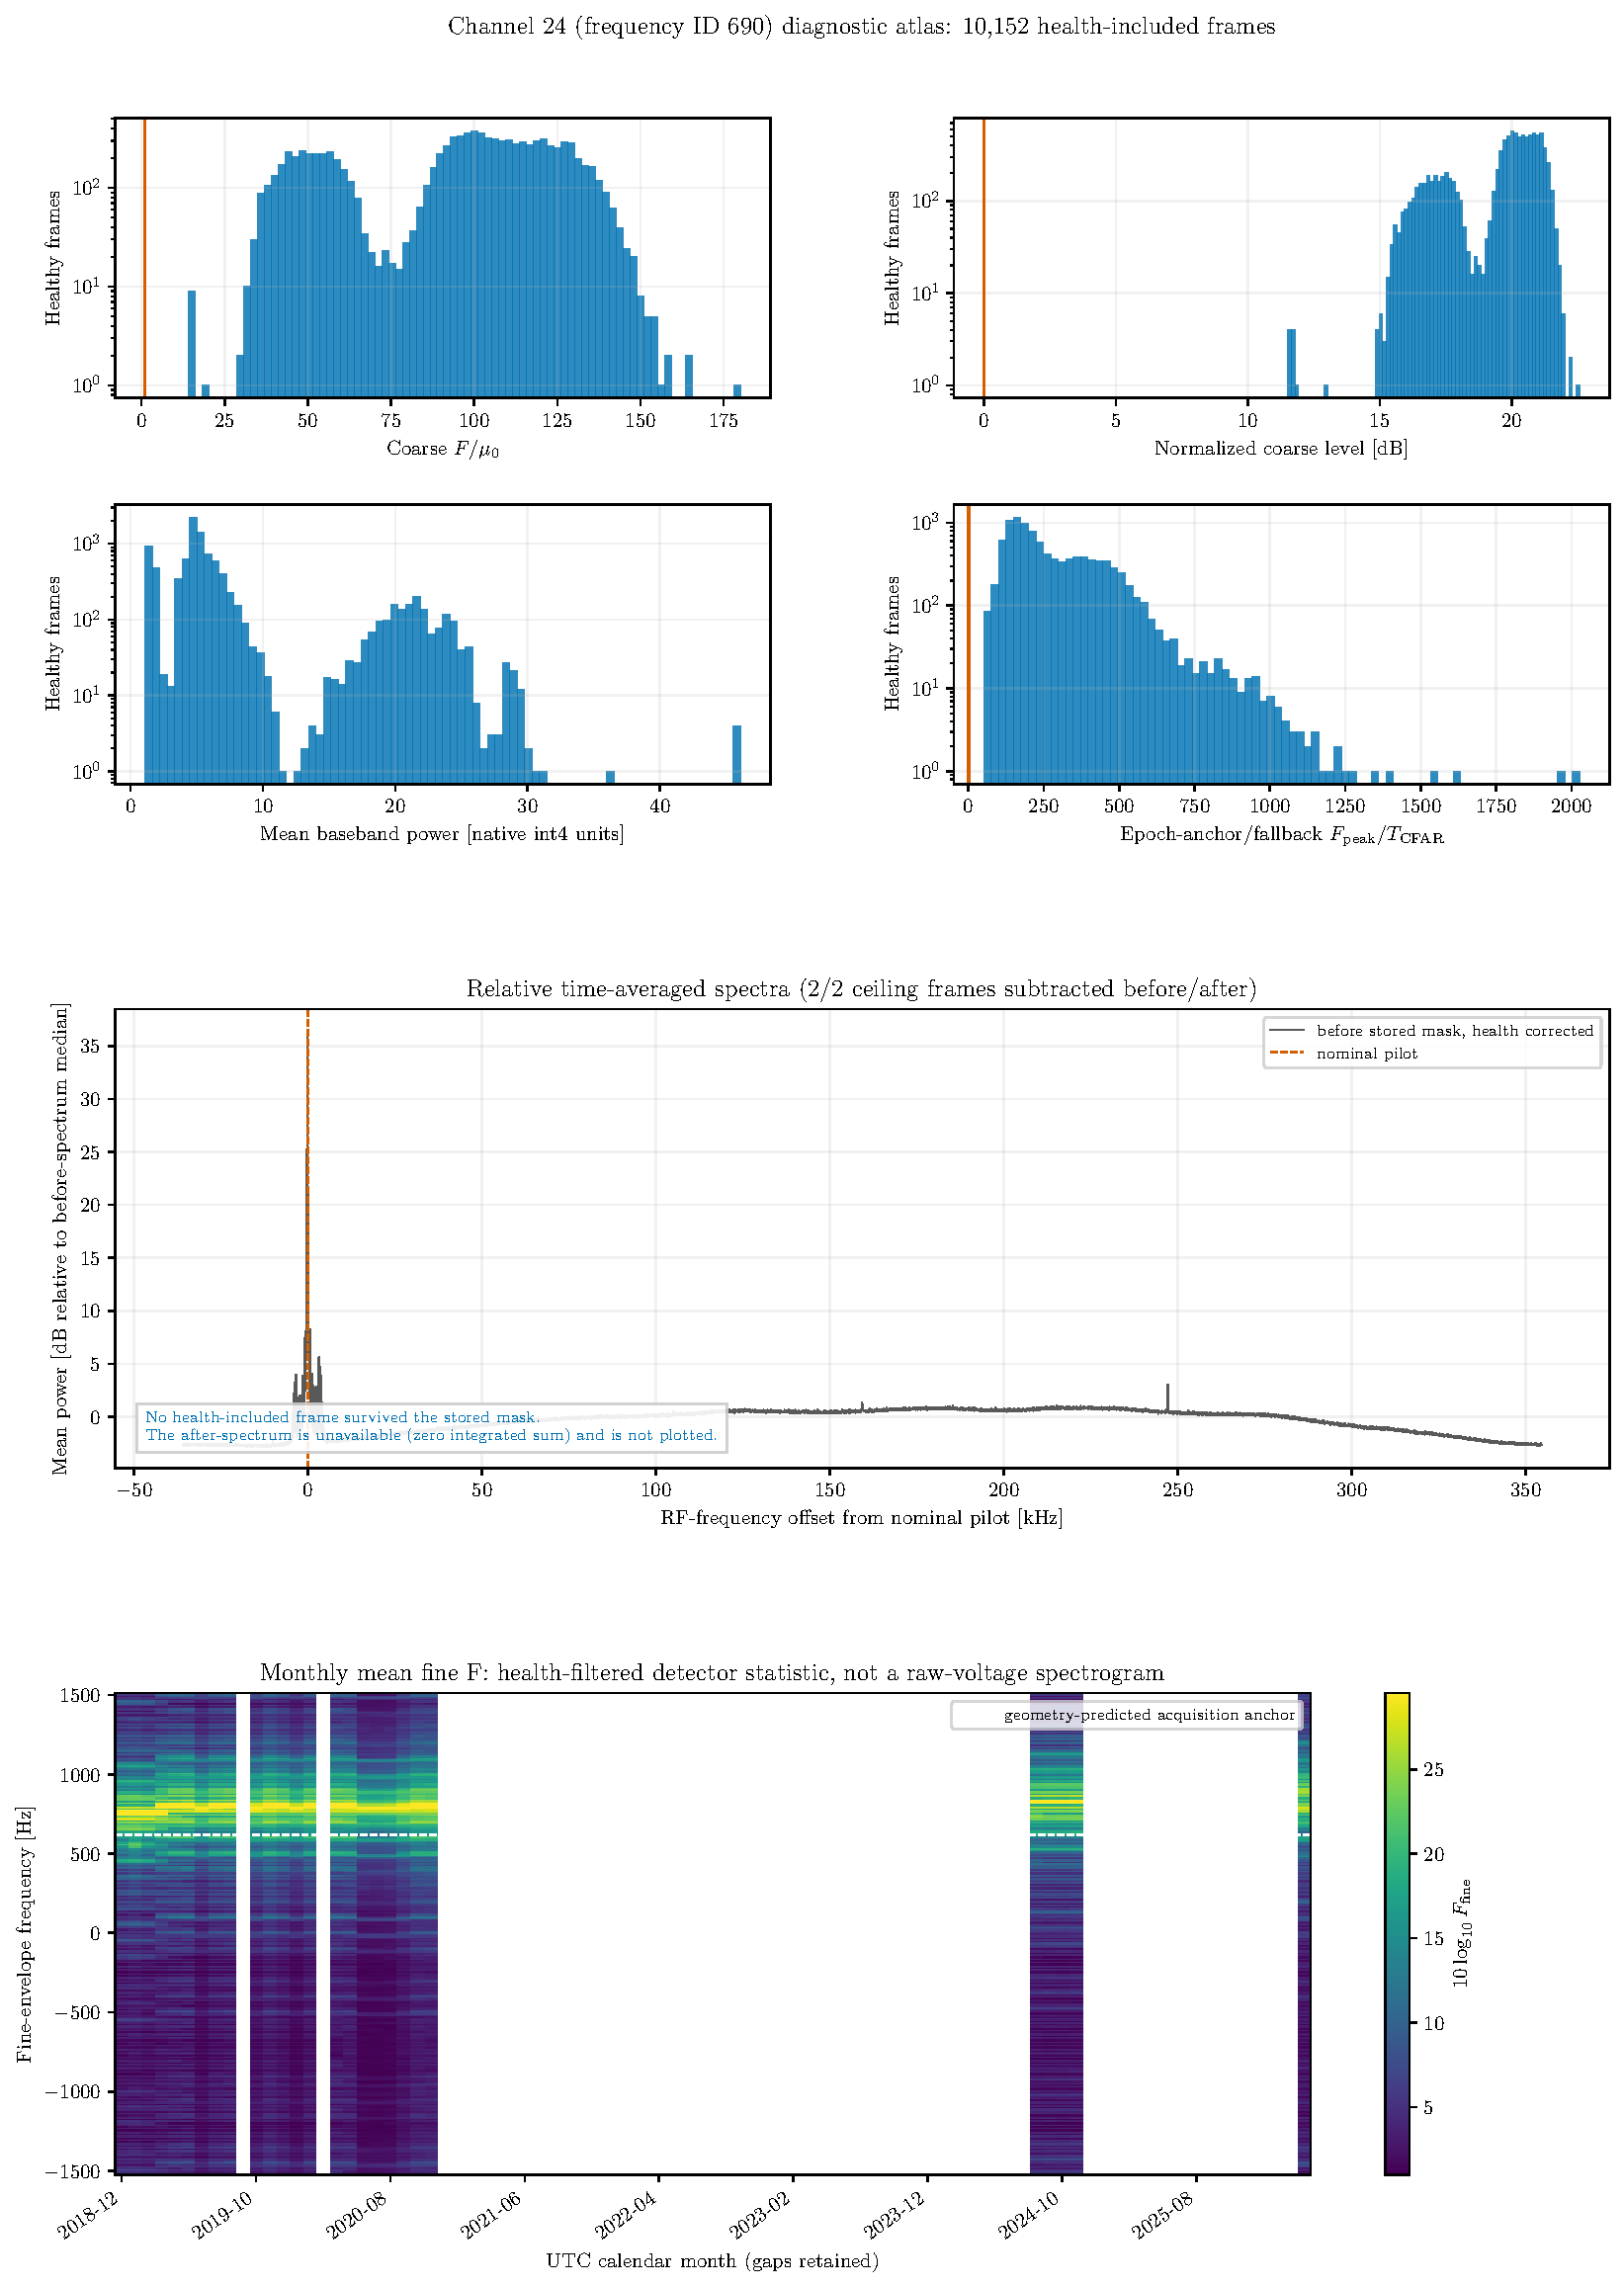
\includegraphics[width=0.98\linewidth,height=0.82\textheight,keepaspectratio]{figs/archive_health_v1/channel_24_diagnostic_atlas.pdf}
\caption{Channel 24 (\texttt{freq\_id}=690).  No health-included frame survives the stored coarse mask, so the after-mask spectrum and empirical residual floor are unavailable.}
\label{fig:archive:atlas:24}
\end{figure}
\clearpage

\begin{figure}[p]
\centering
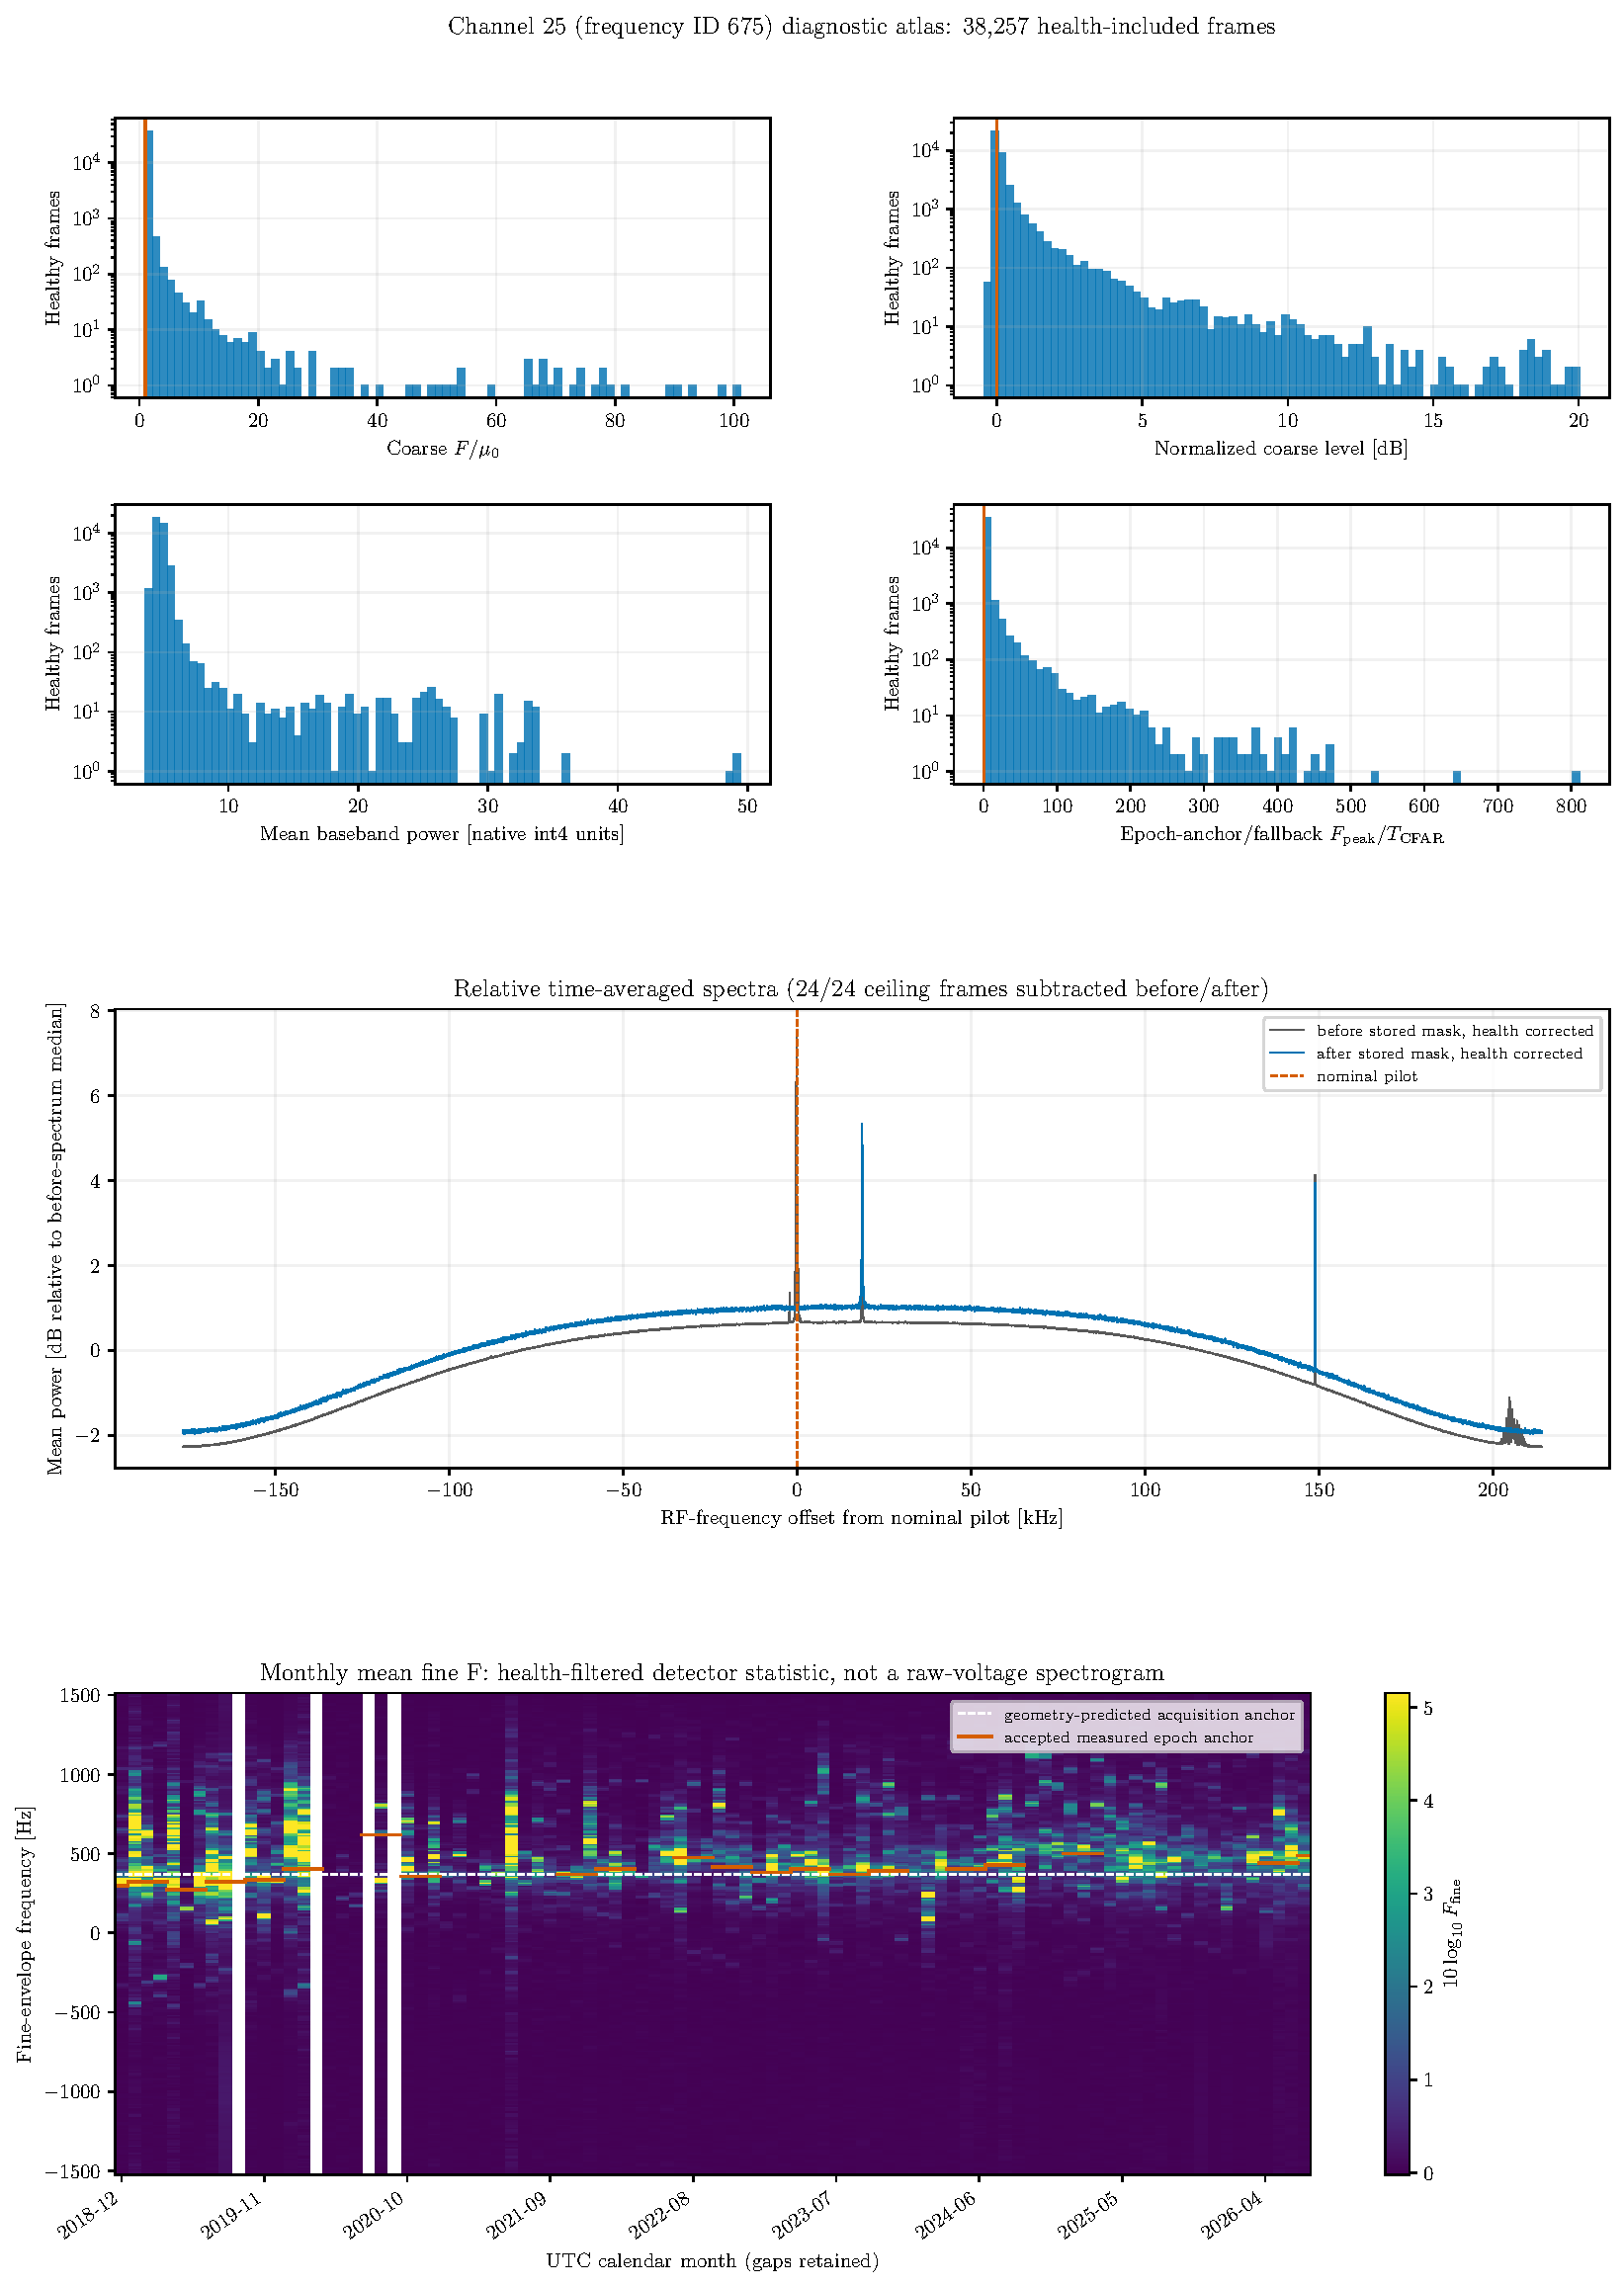
\includegraphics[width=0.98\linewidth,height=0.82\textheight,keepaspectratio]{figs/archive_health_v1/channel_25_diagnostic_atlas.pdf}
\caption{Channel 25 (\texttt{freq\_id}=675) health-filtered archive diagnostics.}
\label{fig:archive:atlas:25}
\end{figure}
\clearpage

\begin{figure}[p]
\centering
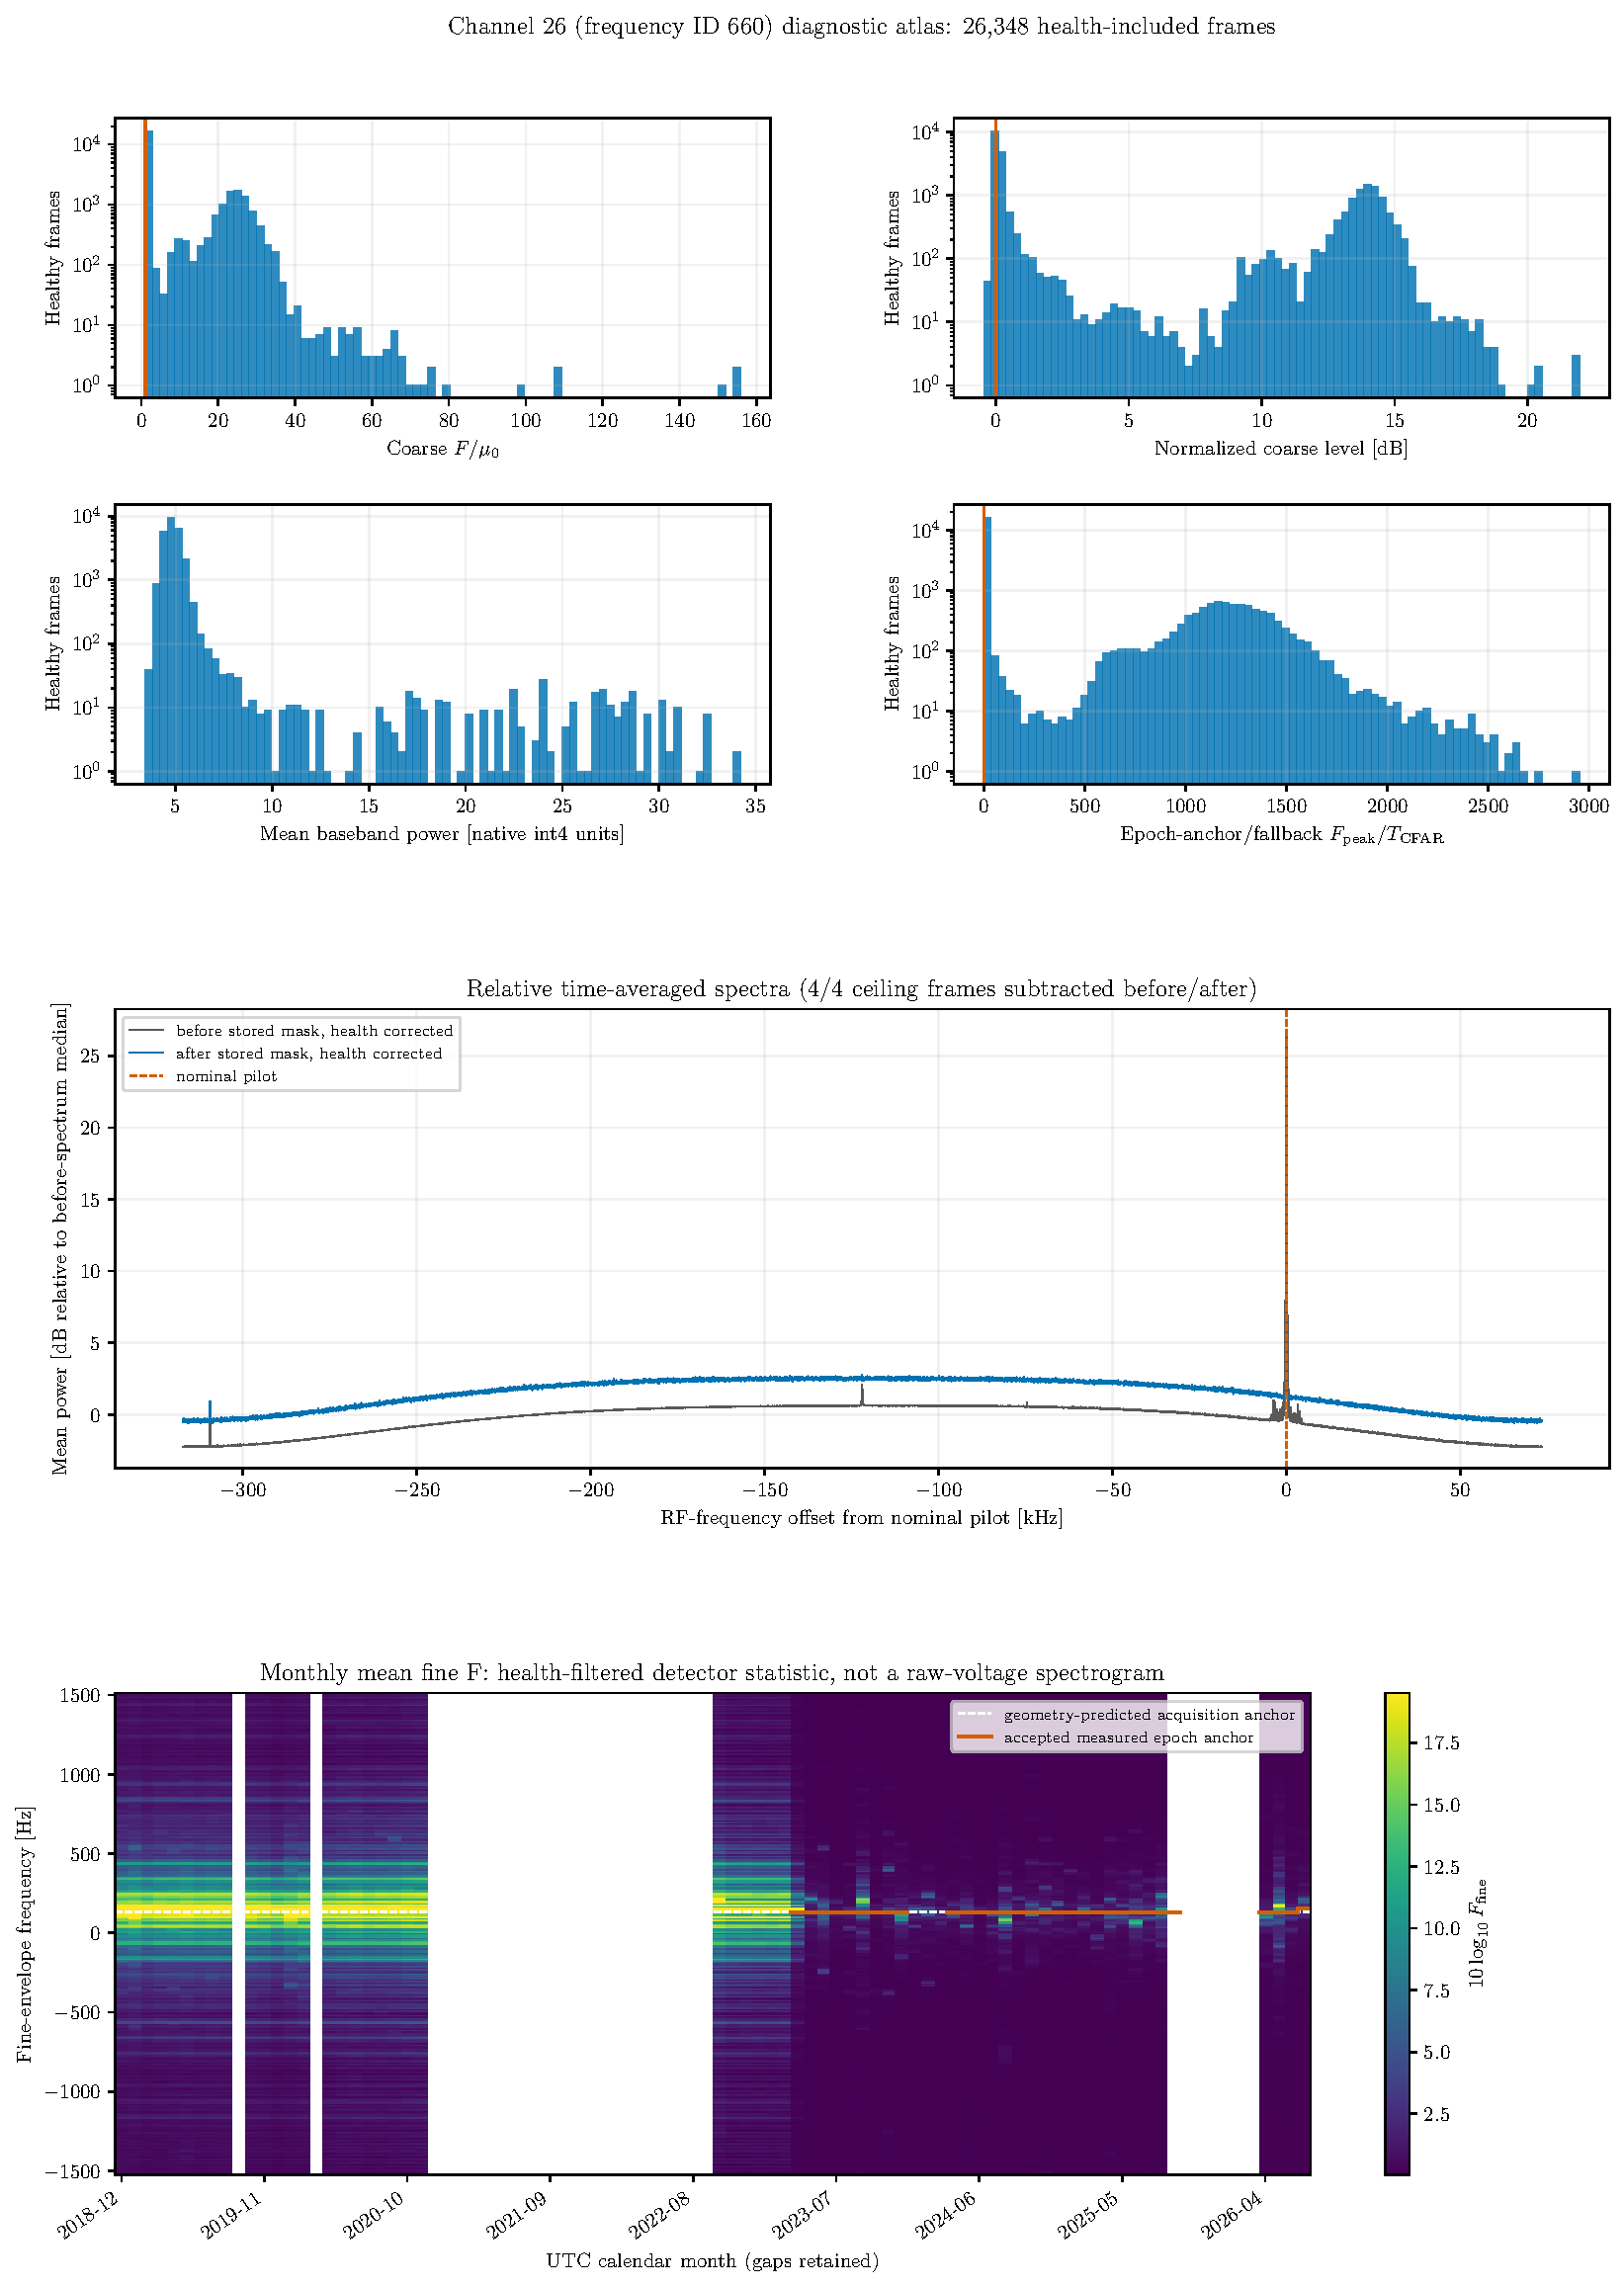
\includegraphics[width=0.98\linewidth,height=0.82\textheight,keepaspectratio]{figs/archive_health_v1/channel_26_diagnostic_atlas.pdf}
\caption{Channel 26 (\texttt{freq\_id}=660) health-filtered archive diagnostics.}
\label{fig:archive:atlas:26}
\end{figure}
\clearpage

\begin{figure}[p]
\centering
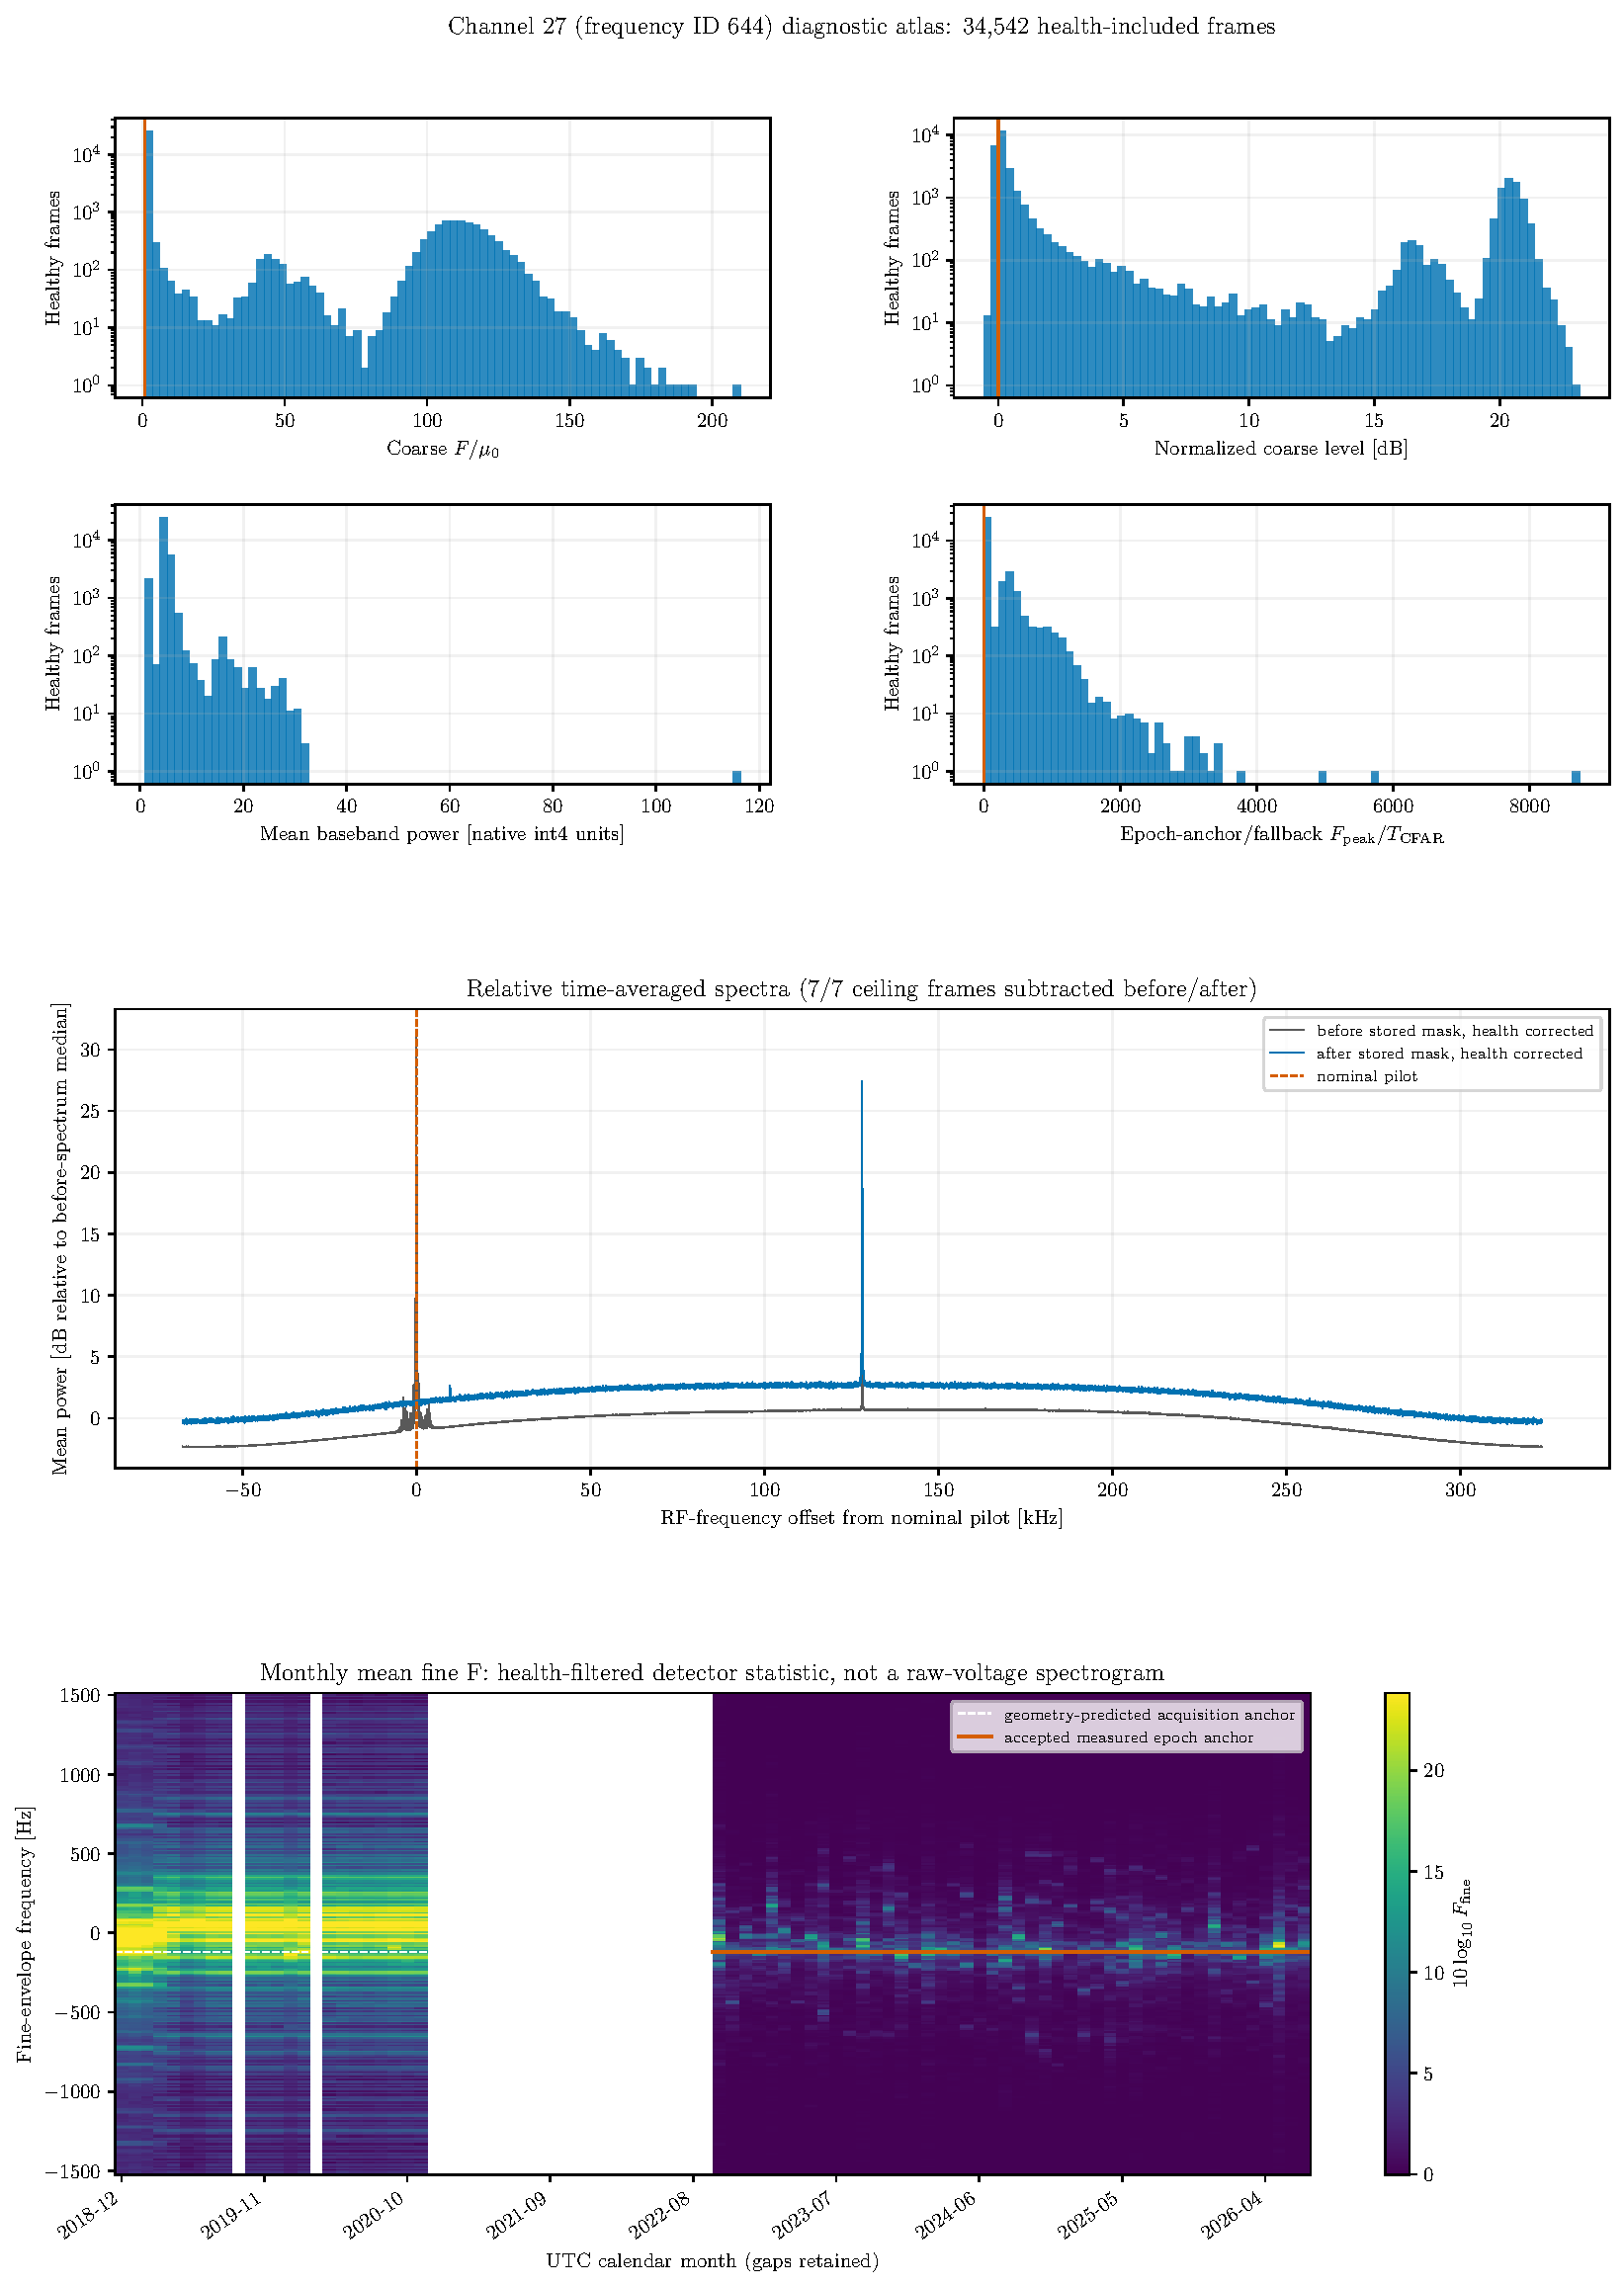
\includegraphics[width=0.98\linewidth,height=0.82\textheight,keepaspectratio]{figs/archive_health_v1/channel_27_diagnostic_atlas.pdf}
\caption{Channel 27 (\texttt{freq\_id}=644) health-filtered archive diagnostics.}
\label{fig:archive:atlas:27}
\end{figure}
\clearpage

\begin{figure}[p]
\centering
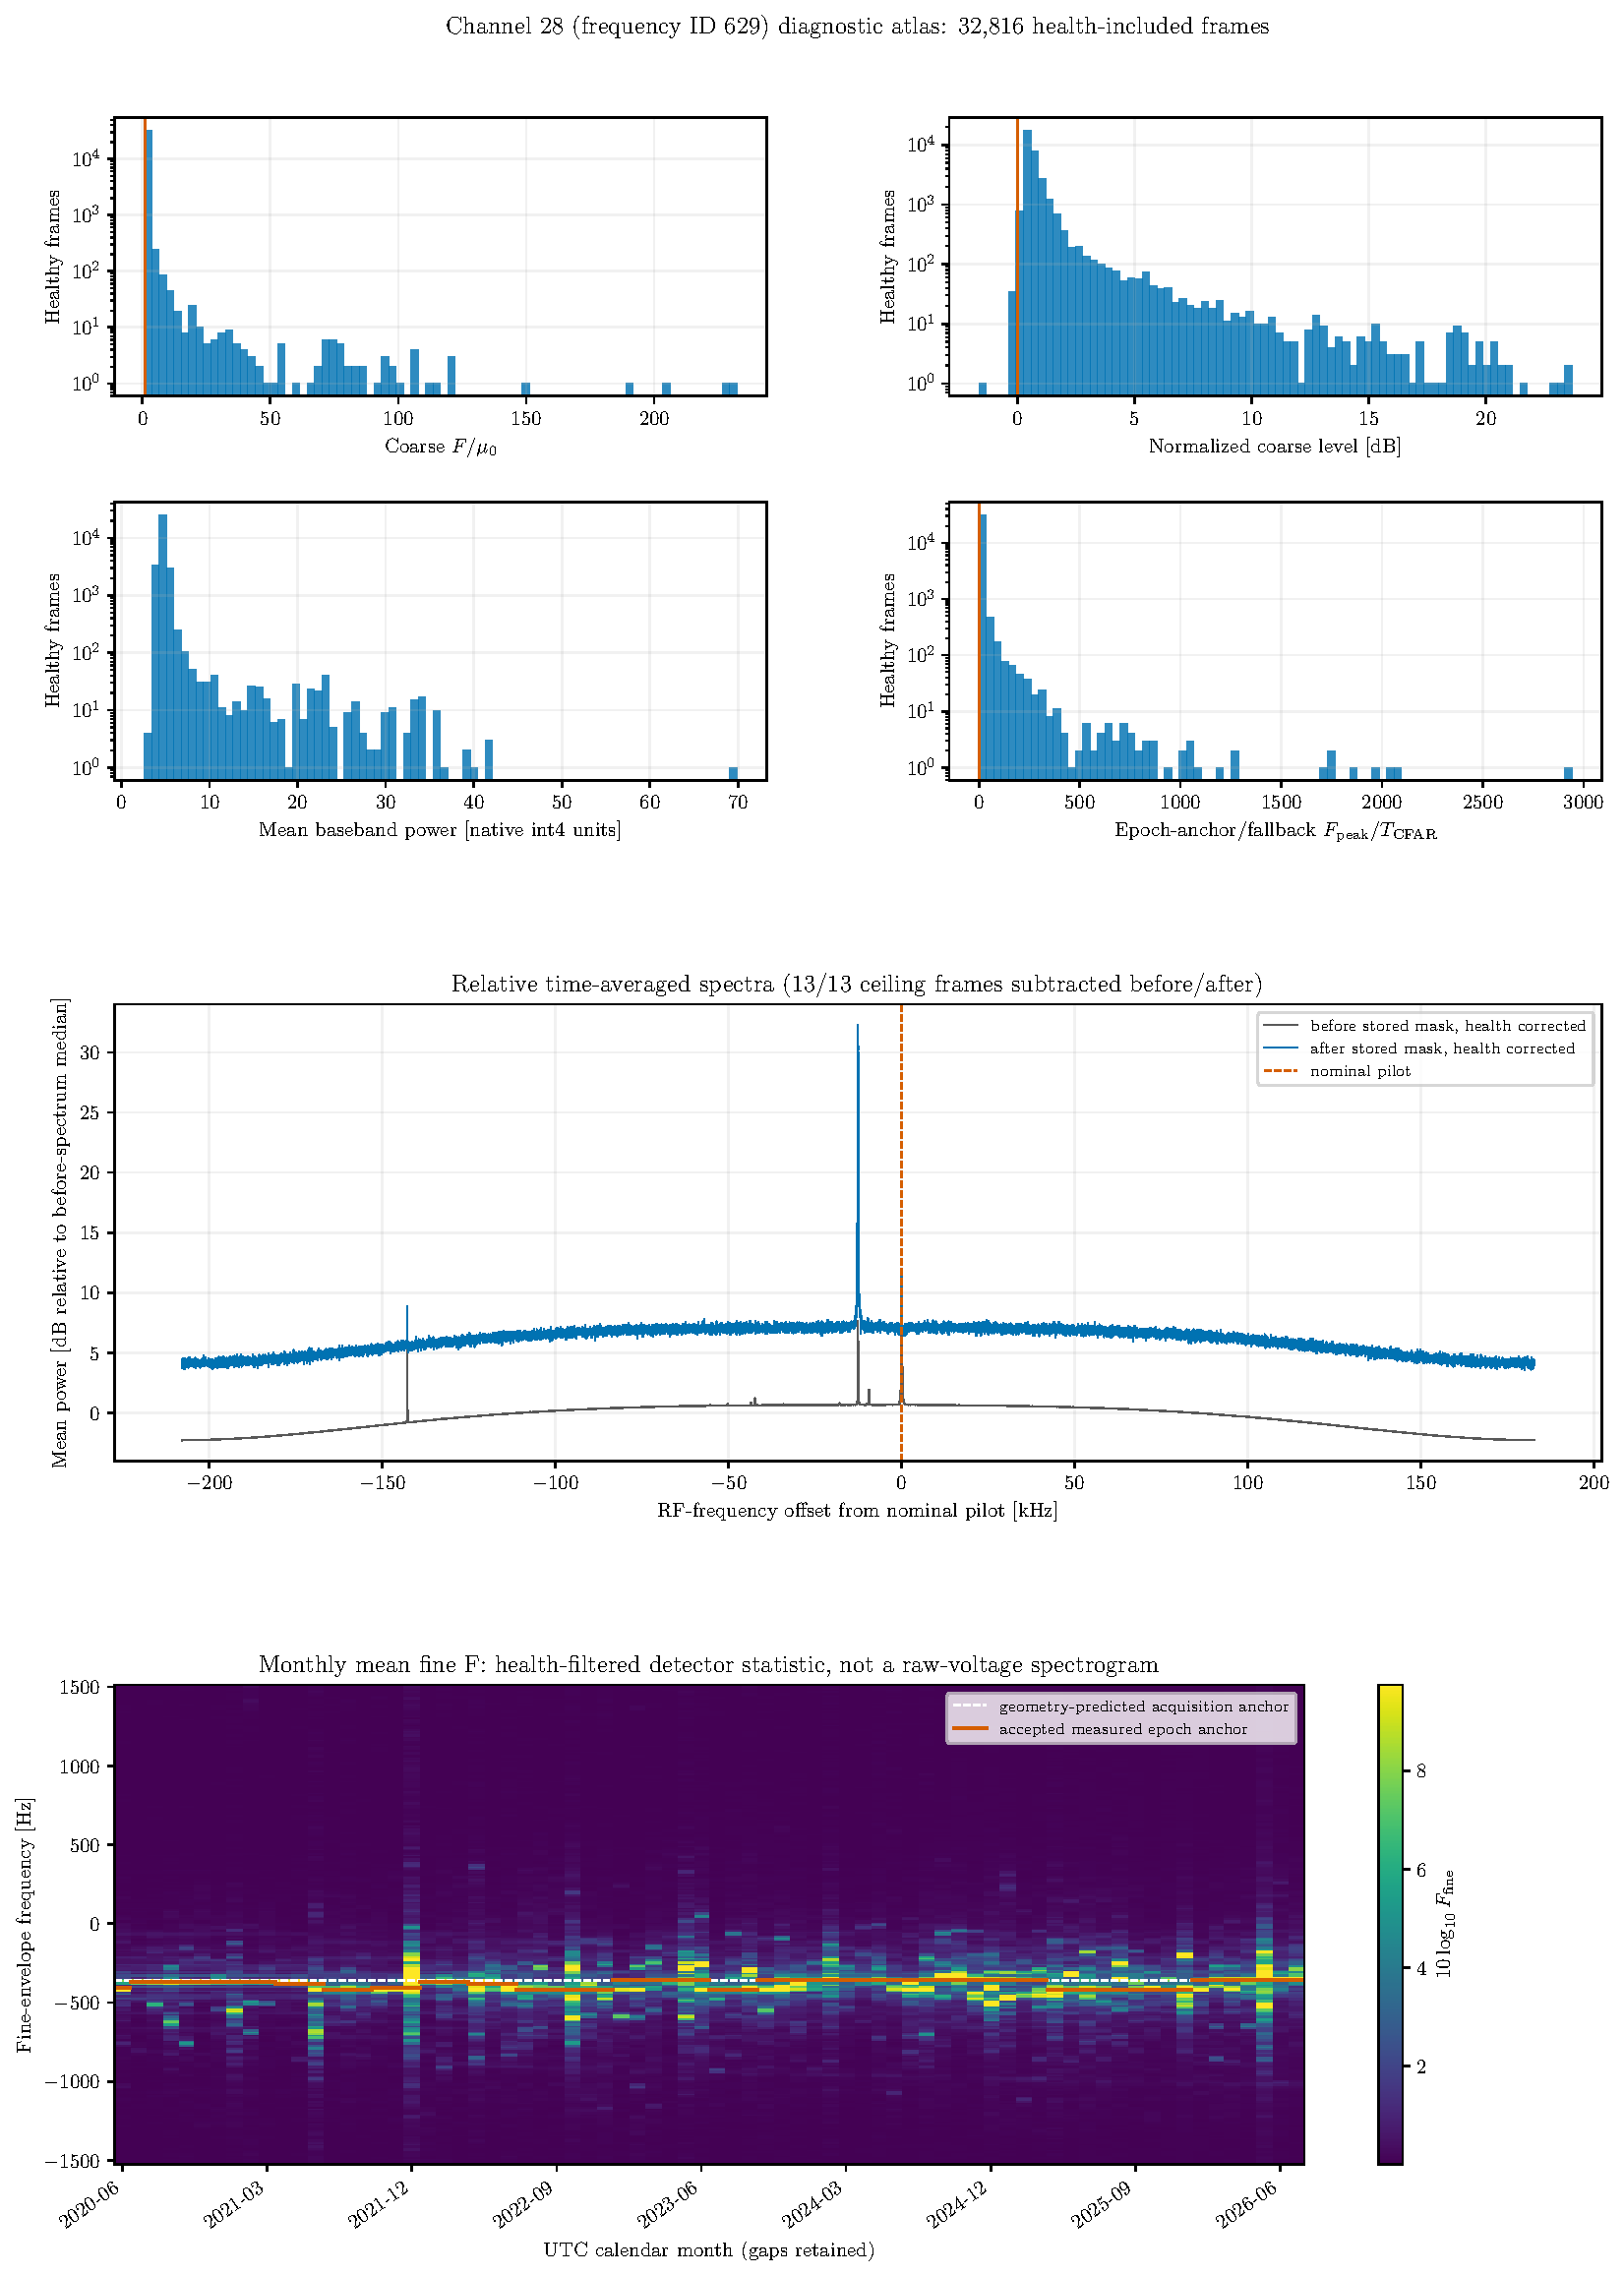
\includegraphics[width=0.98\linewidth,height=0.82\textheight,keepaspectratio]{figs/archive_health_v1/channel_28_diagnostic_atlas.pdf}
\caption{Channel 28 (\texttt{freq\_id}=629) health-filtered archive diagnostics.}
\label{fig:archive:atlas:28}
\end{figure}
\clearpage

\begin{figure}[p]
\centering
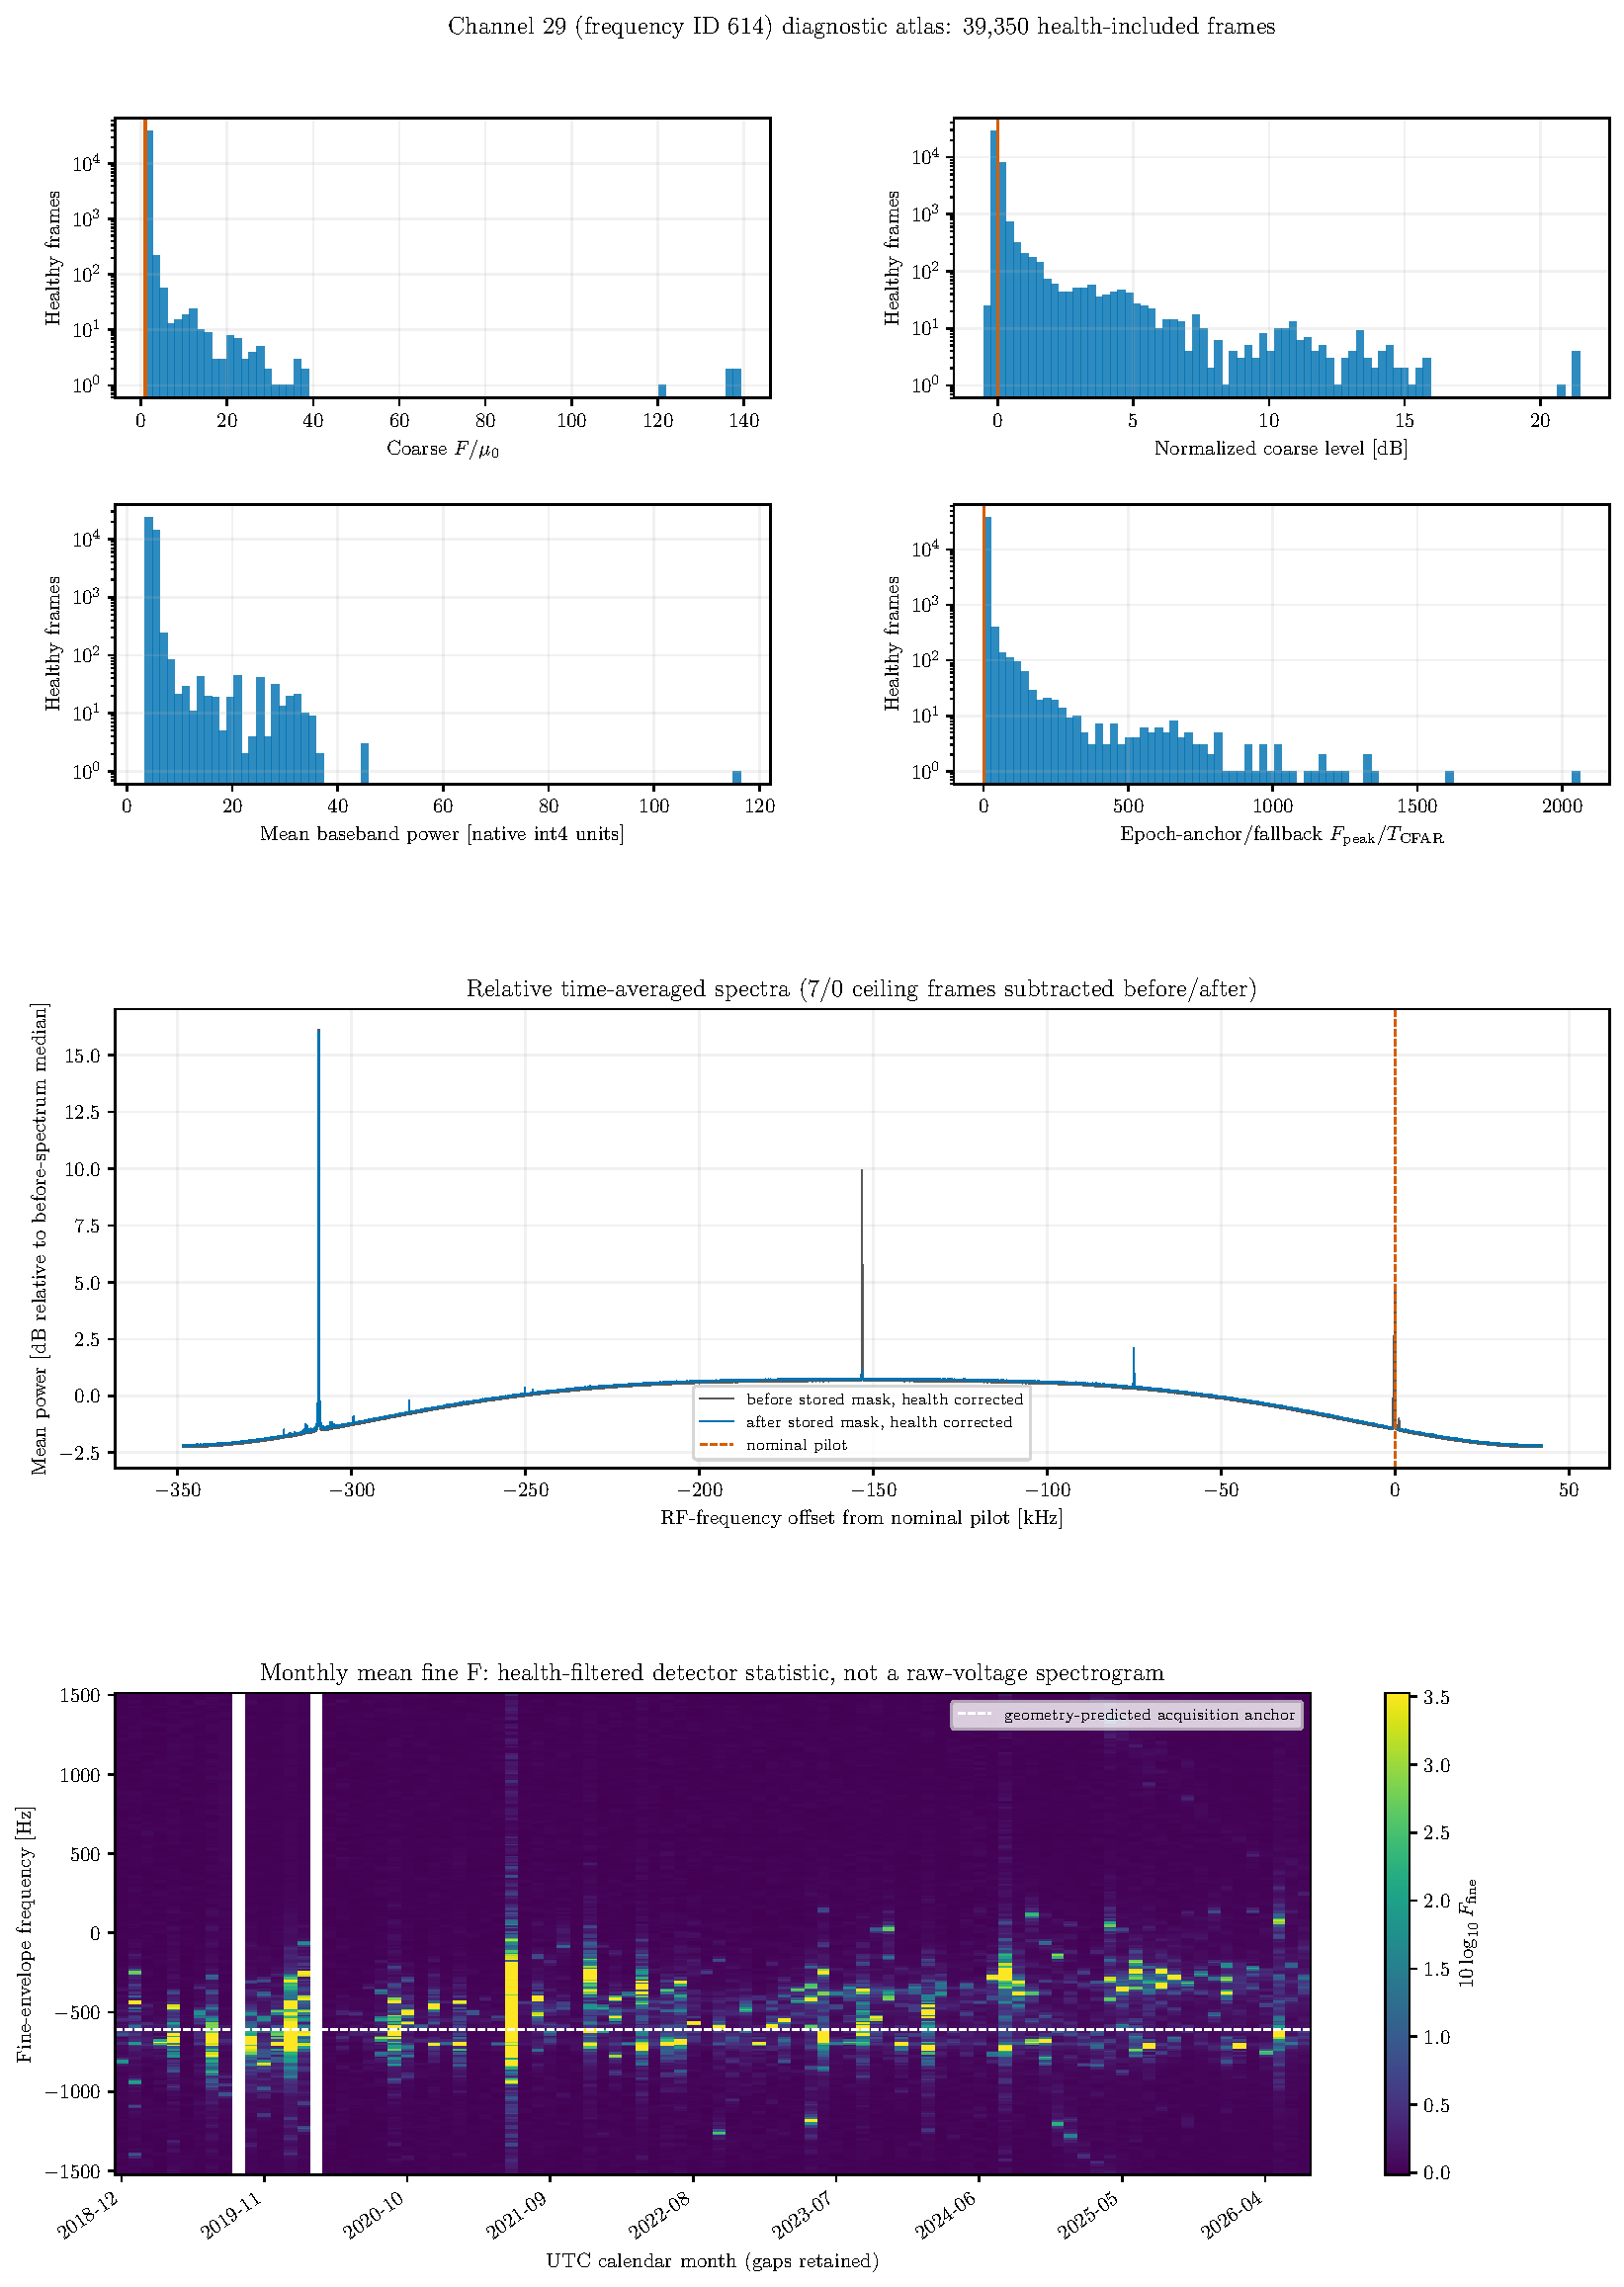
\includegraphics[width=0.98\linewidth,height=0.82\textheight,keepaspectratio]{figs/archive_health_v1/channel_29_diagnostic_atlas.pdf}
\caption{Channel 29 (\texttt{freq\_id}=614) health-filtered archive diagnostics.}
\label{fig:archive:atlas:29}
\end{figure}
\clearpage

\begin{figure}[p]
\centering
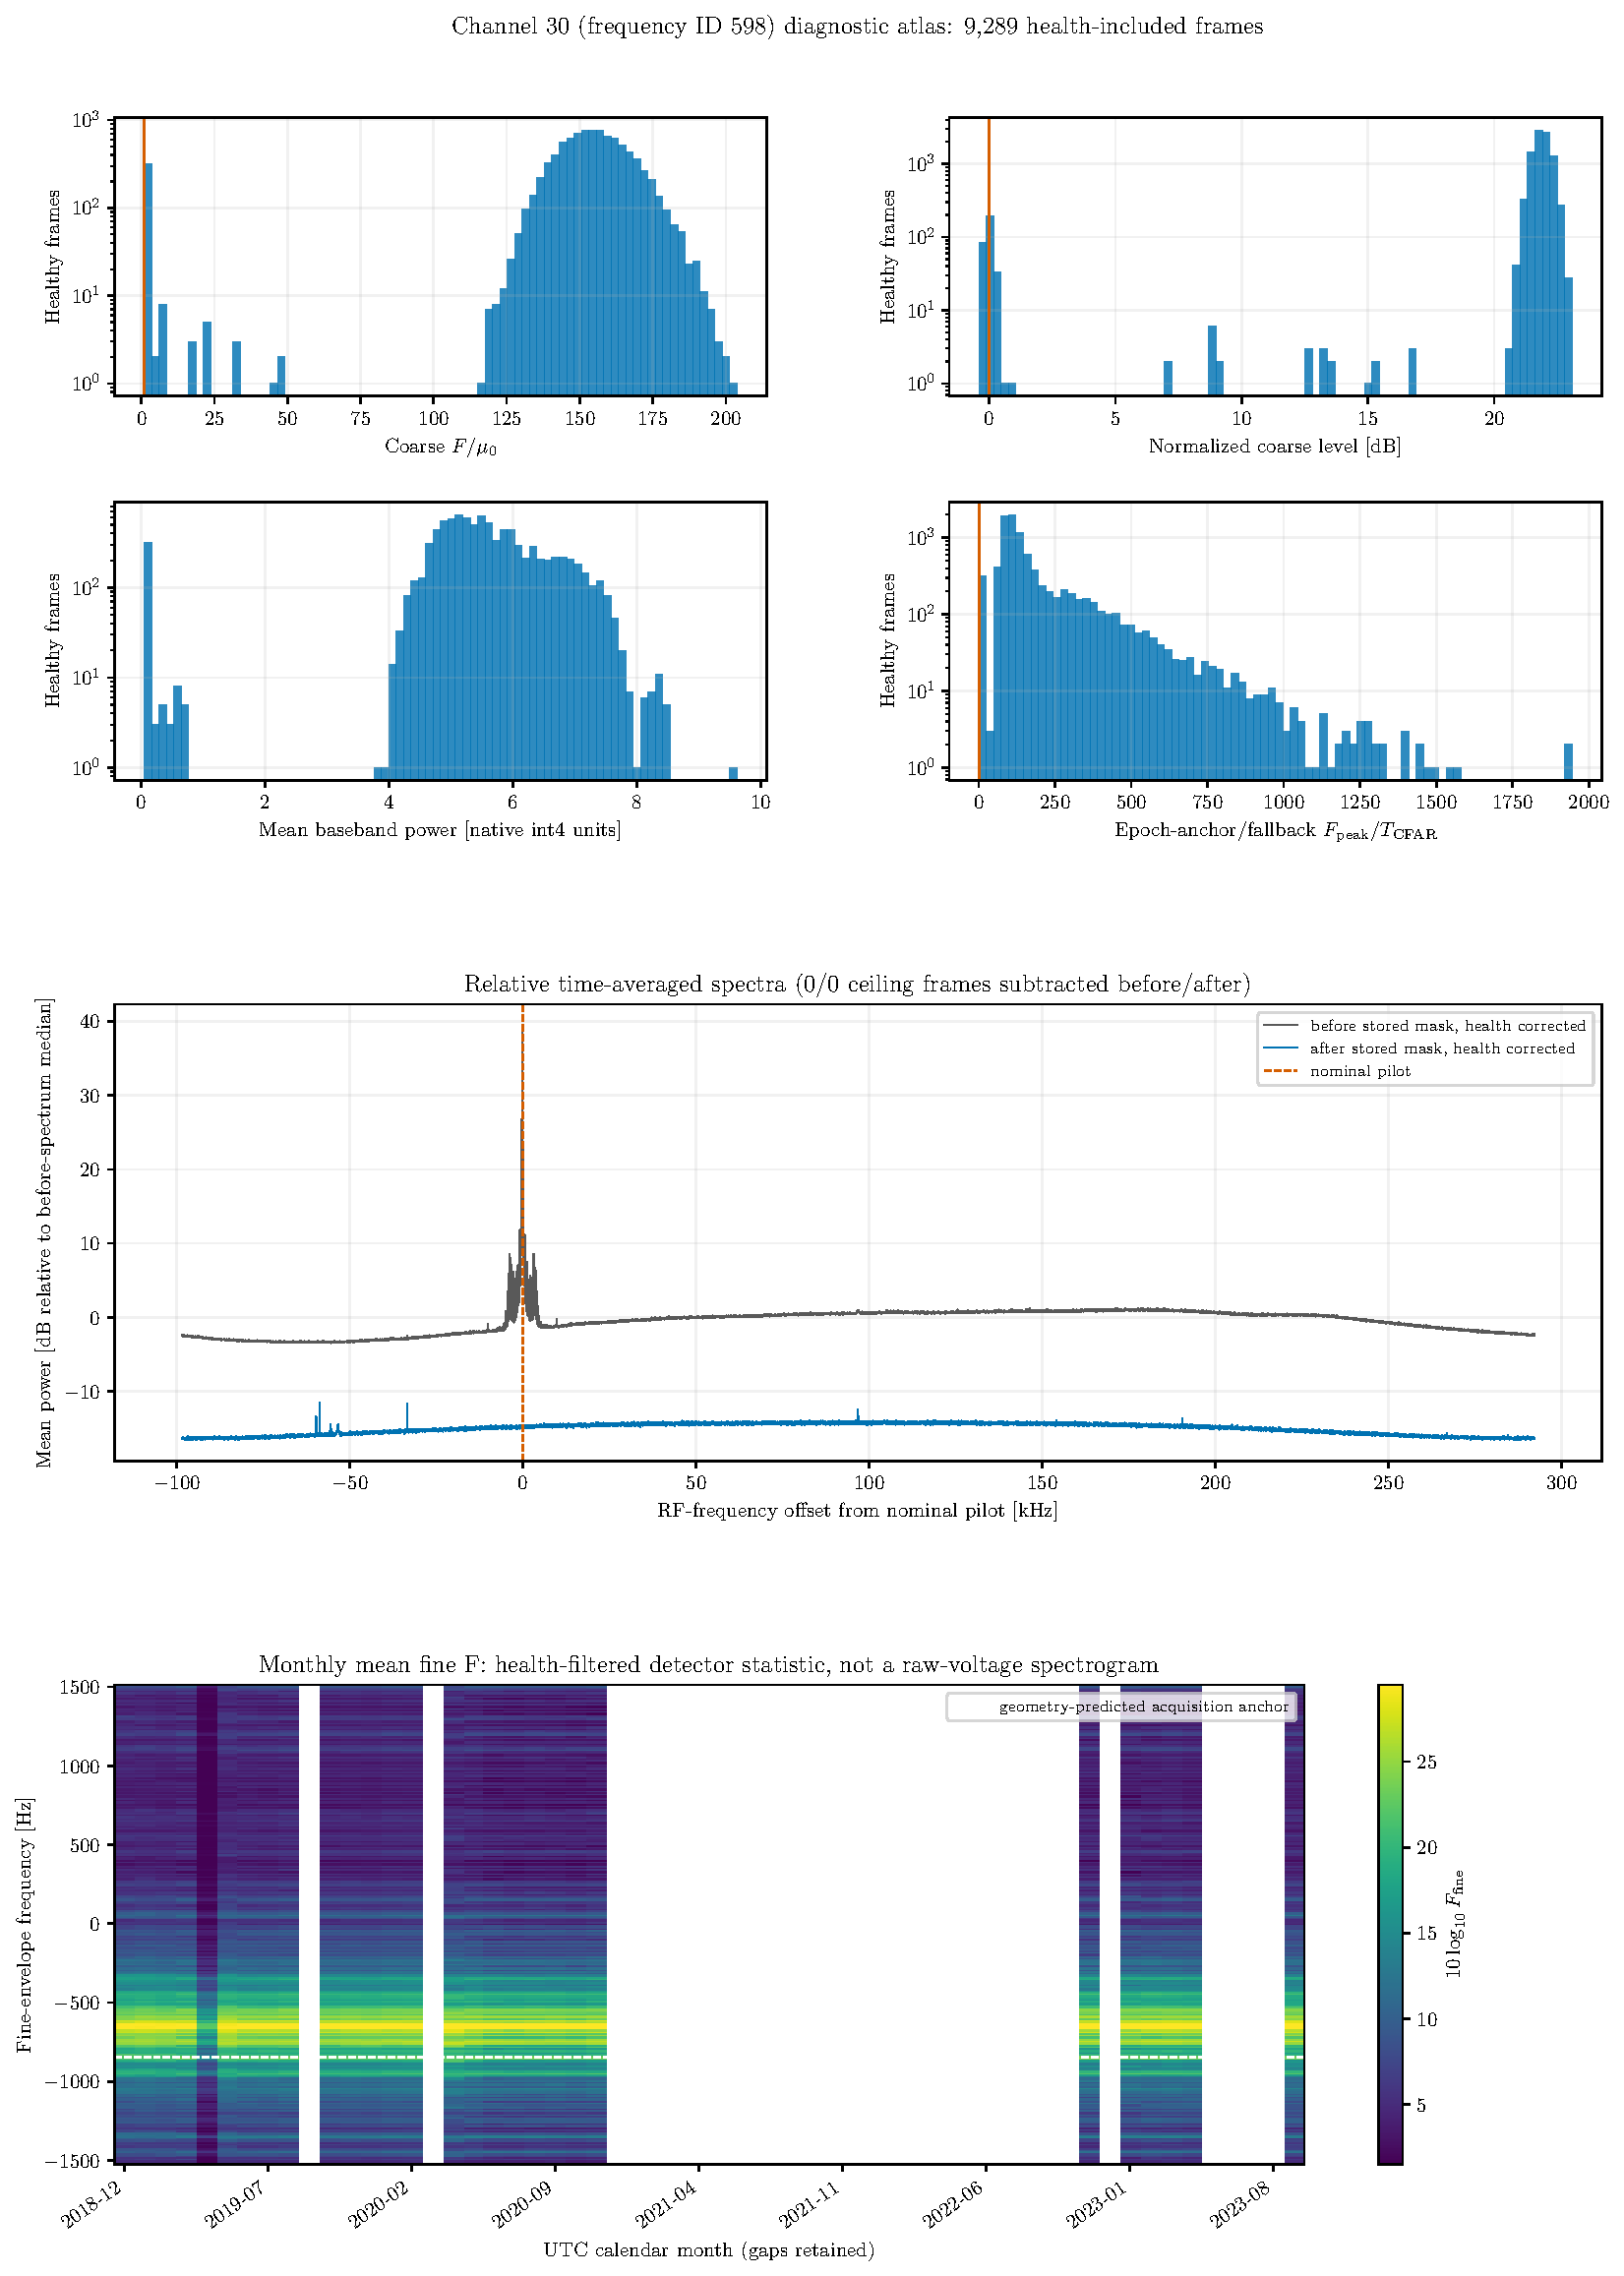
\includegraphics[width=0.98\linewidth,height=0.82\textheight,keepaspectratio]{figs/archive_health_v1/channel_30_diagnostic_atlas.pdf}
\caption{Channel 30 (\texttt{freq\_id}=598).  The plate describes the archive through September 2023; it does not resolve the channel's later operating state.}
\label{fig:archive:atlas:30}
\end{figure}
\clearpage

\begin{figure}[p]
\centering
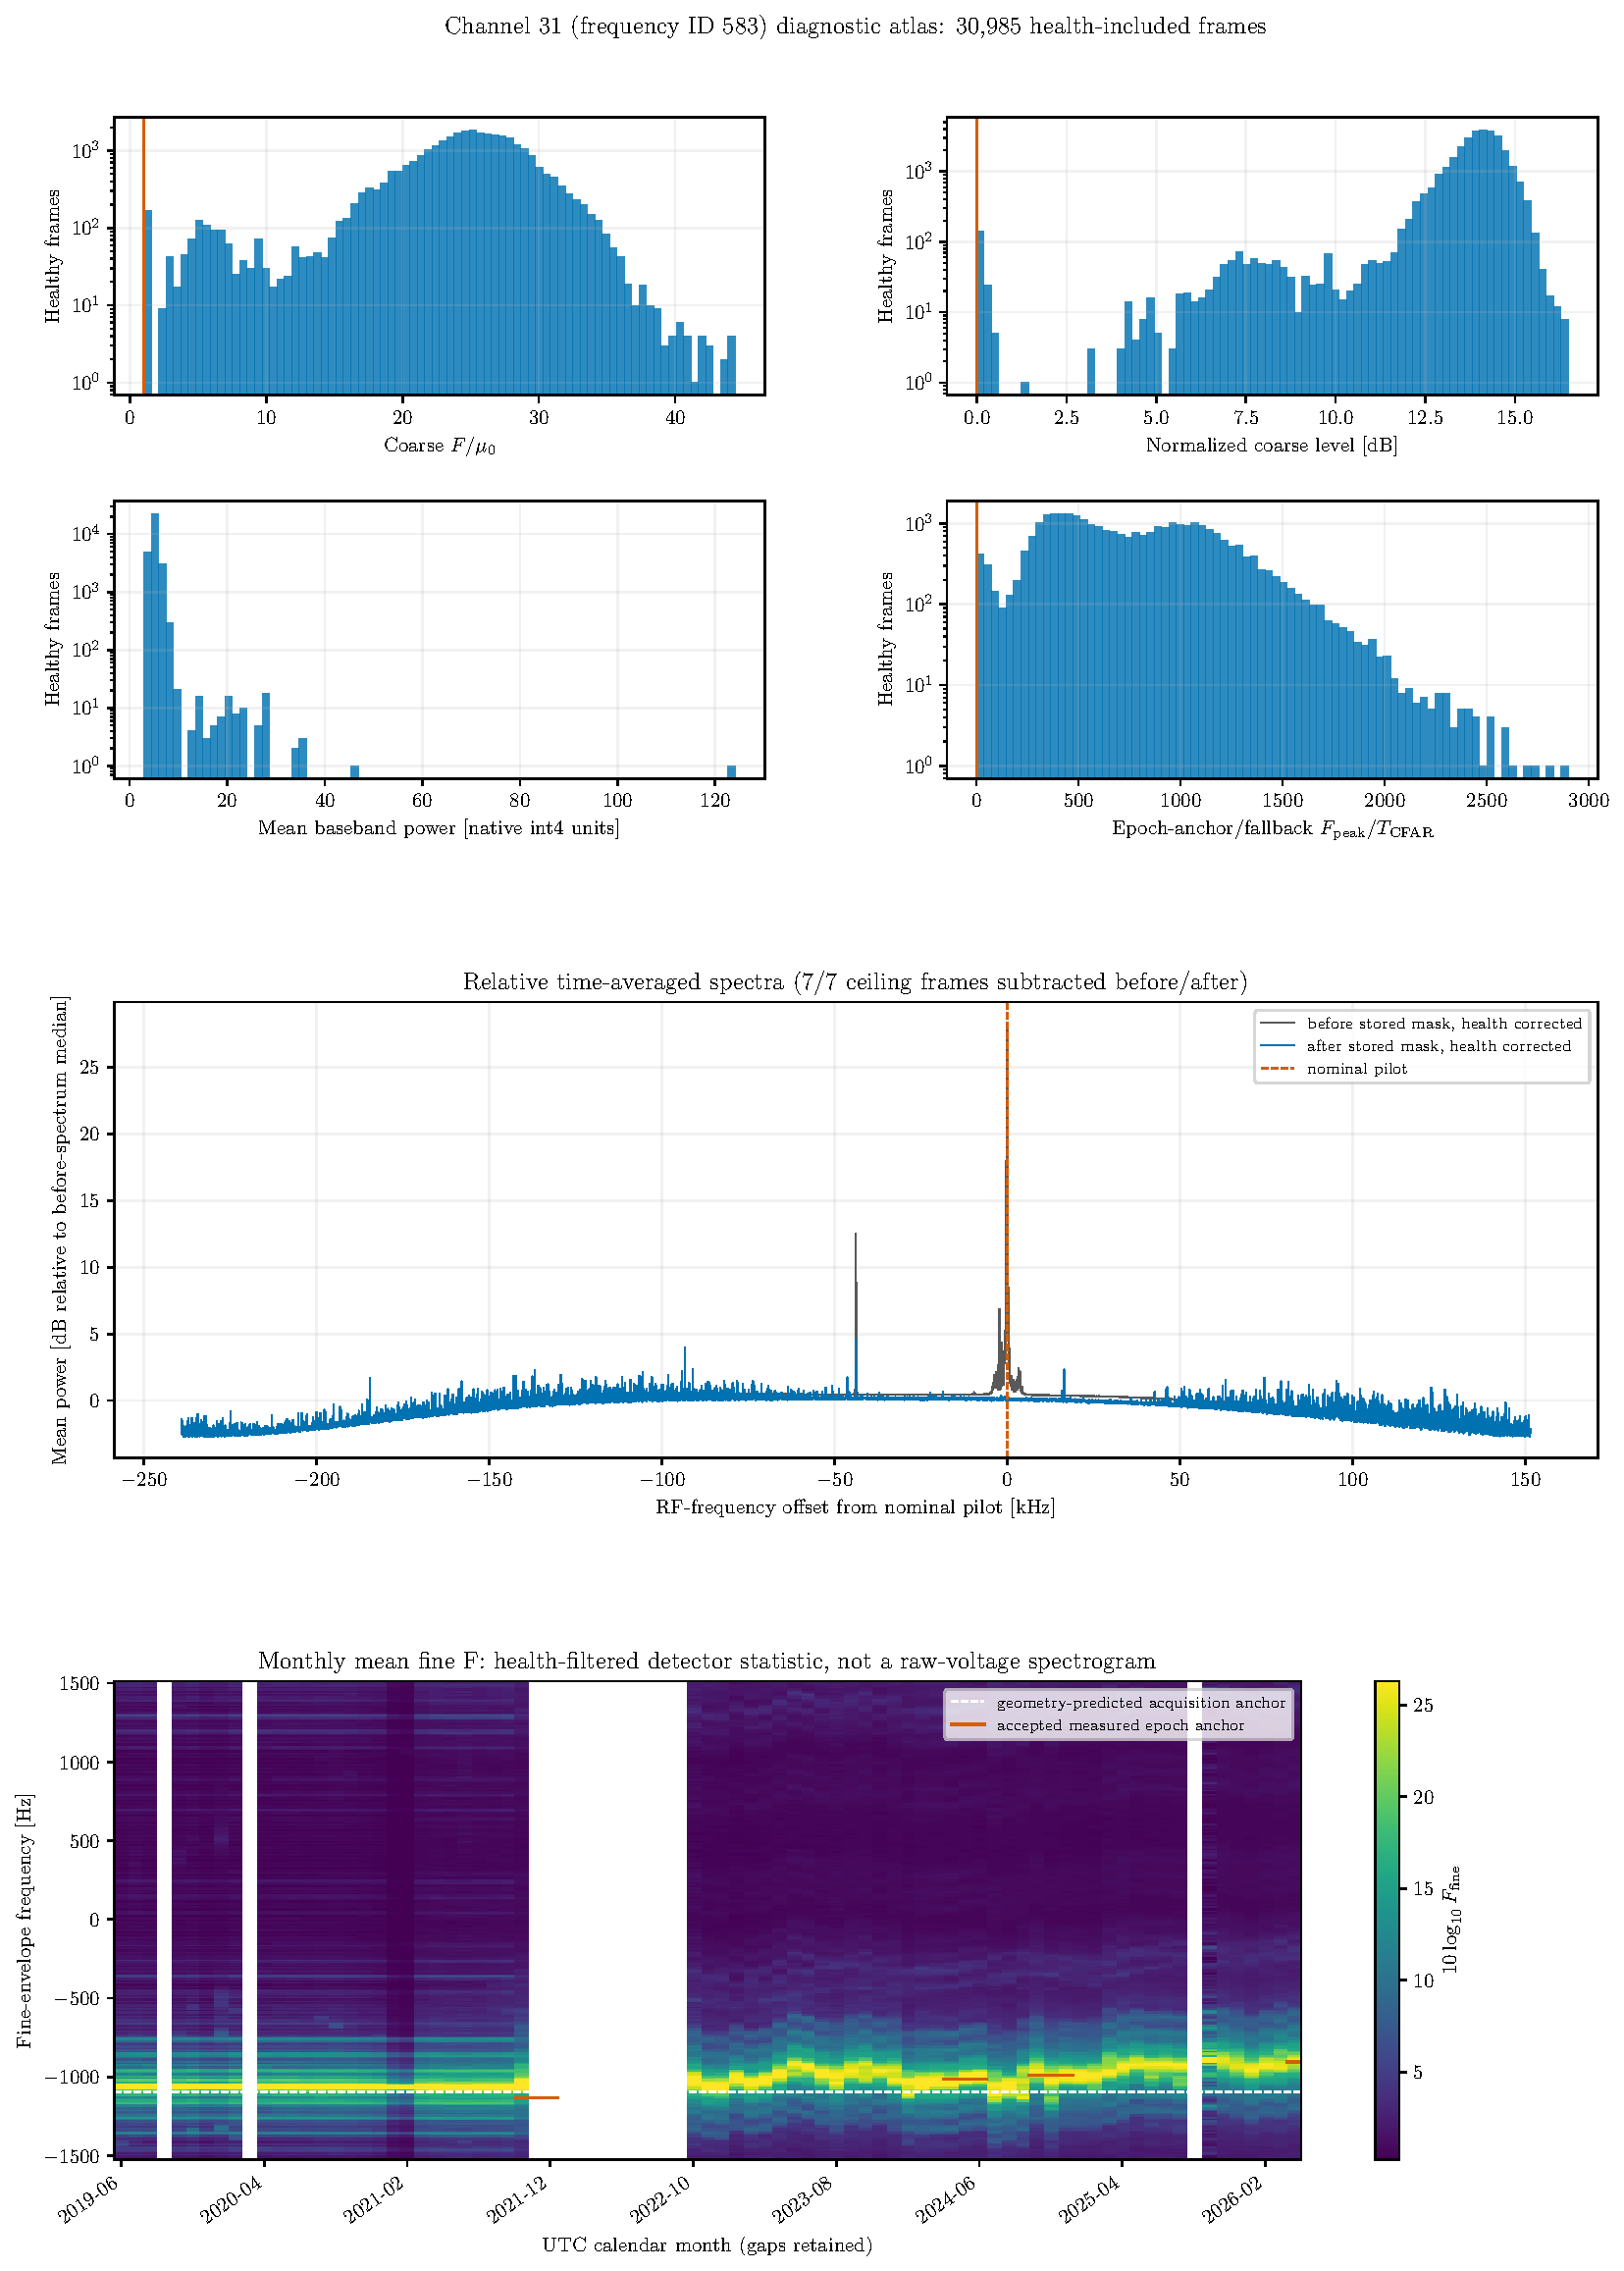
\includegraphics[width=0.98\linewidth,height=0.82\textheight,keepaspectratio]{figs/archive_health_v1/channel_31_diagnostic_atlas.pdf}
\caption{Channel 31 (\texttt{freq\_id}=583) health-filtered archive diagnostics.}
\label{fig:archive:atlas:31}
\end{figure}
\clearpage

\begin{figure}[p]
\centering
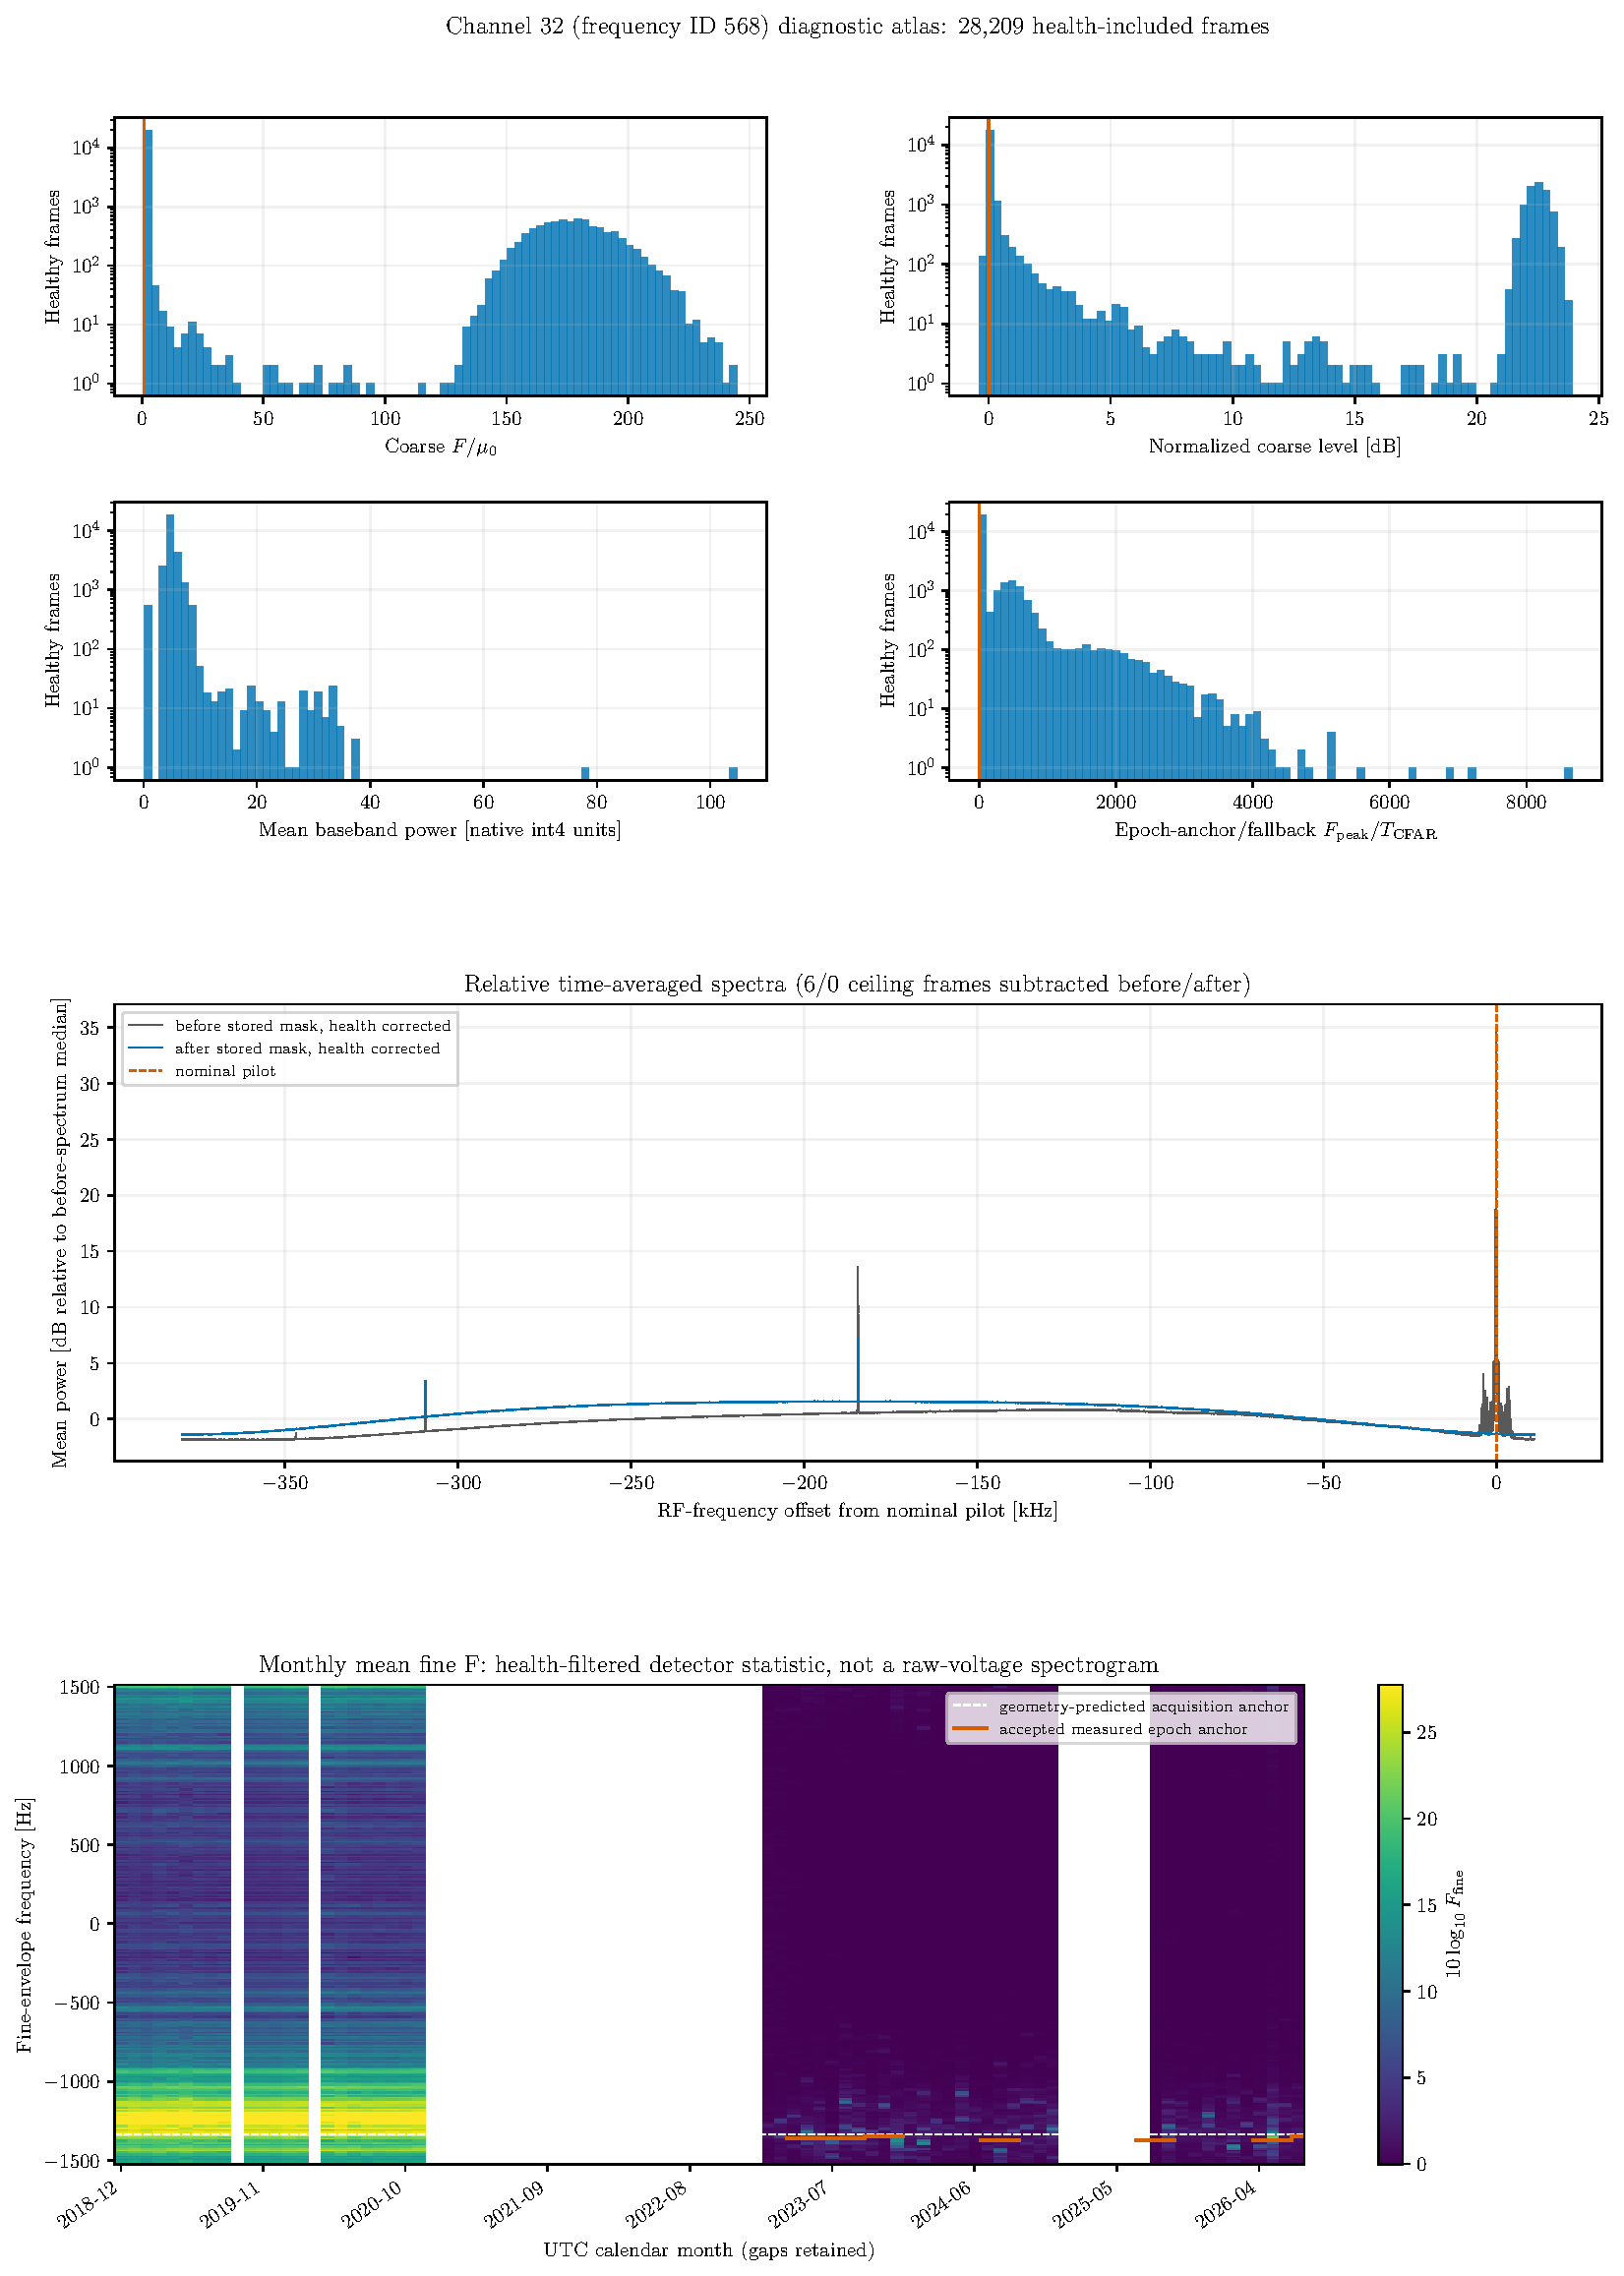
\includegraphics[width=0.98\linewidth,height=0.82\textheight,keepaspectratio]{figs/archive_health_v1/channel_32_diagnostic_atlas.pdf}
\caption{Channel 32 (\texttt{freq\_id}=568) health-filtered archive diagnostics.}
\label{fig:archive:atlas:32}
\end{figure}
\clearpage

\begin{figure}[p]
\centering
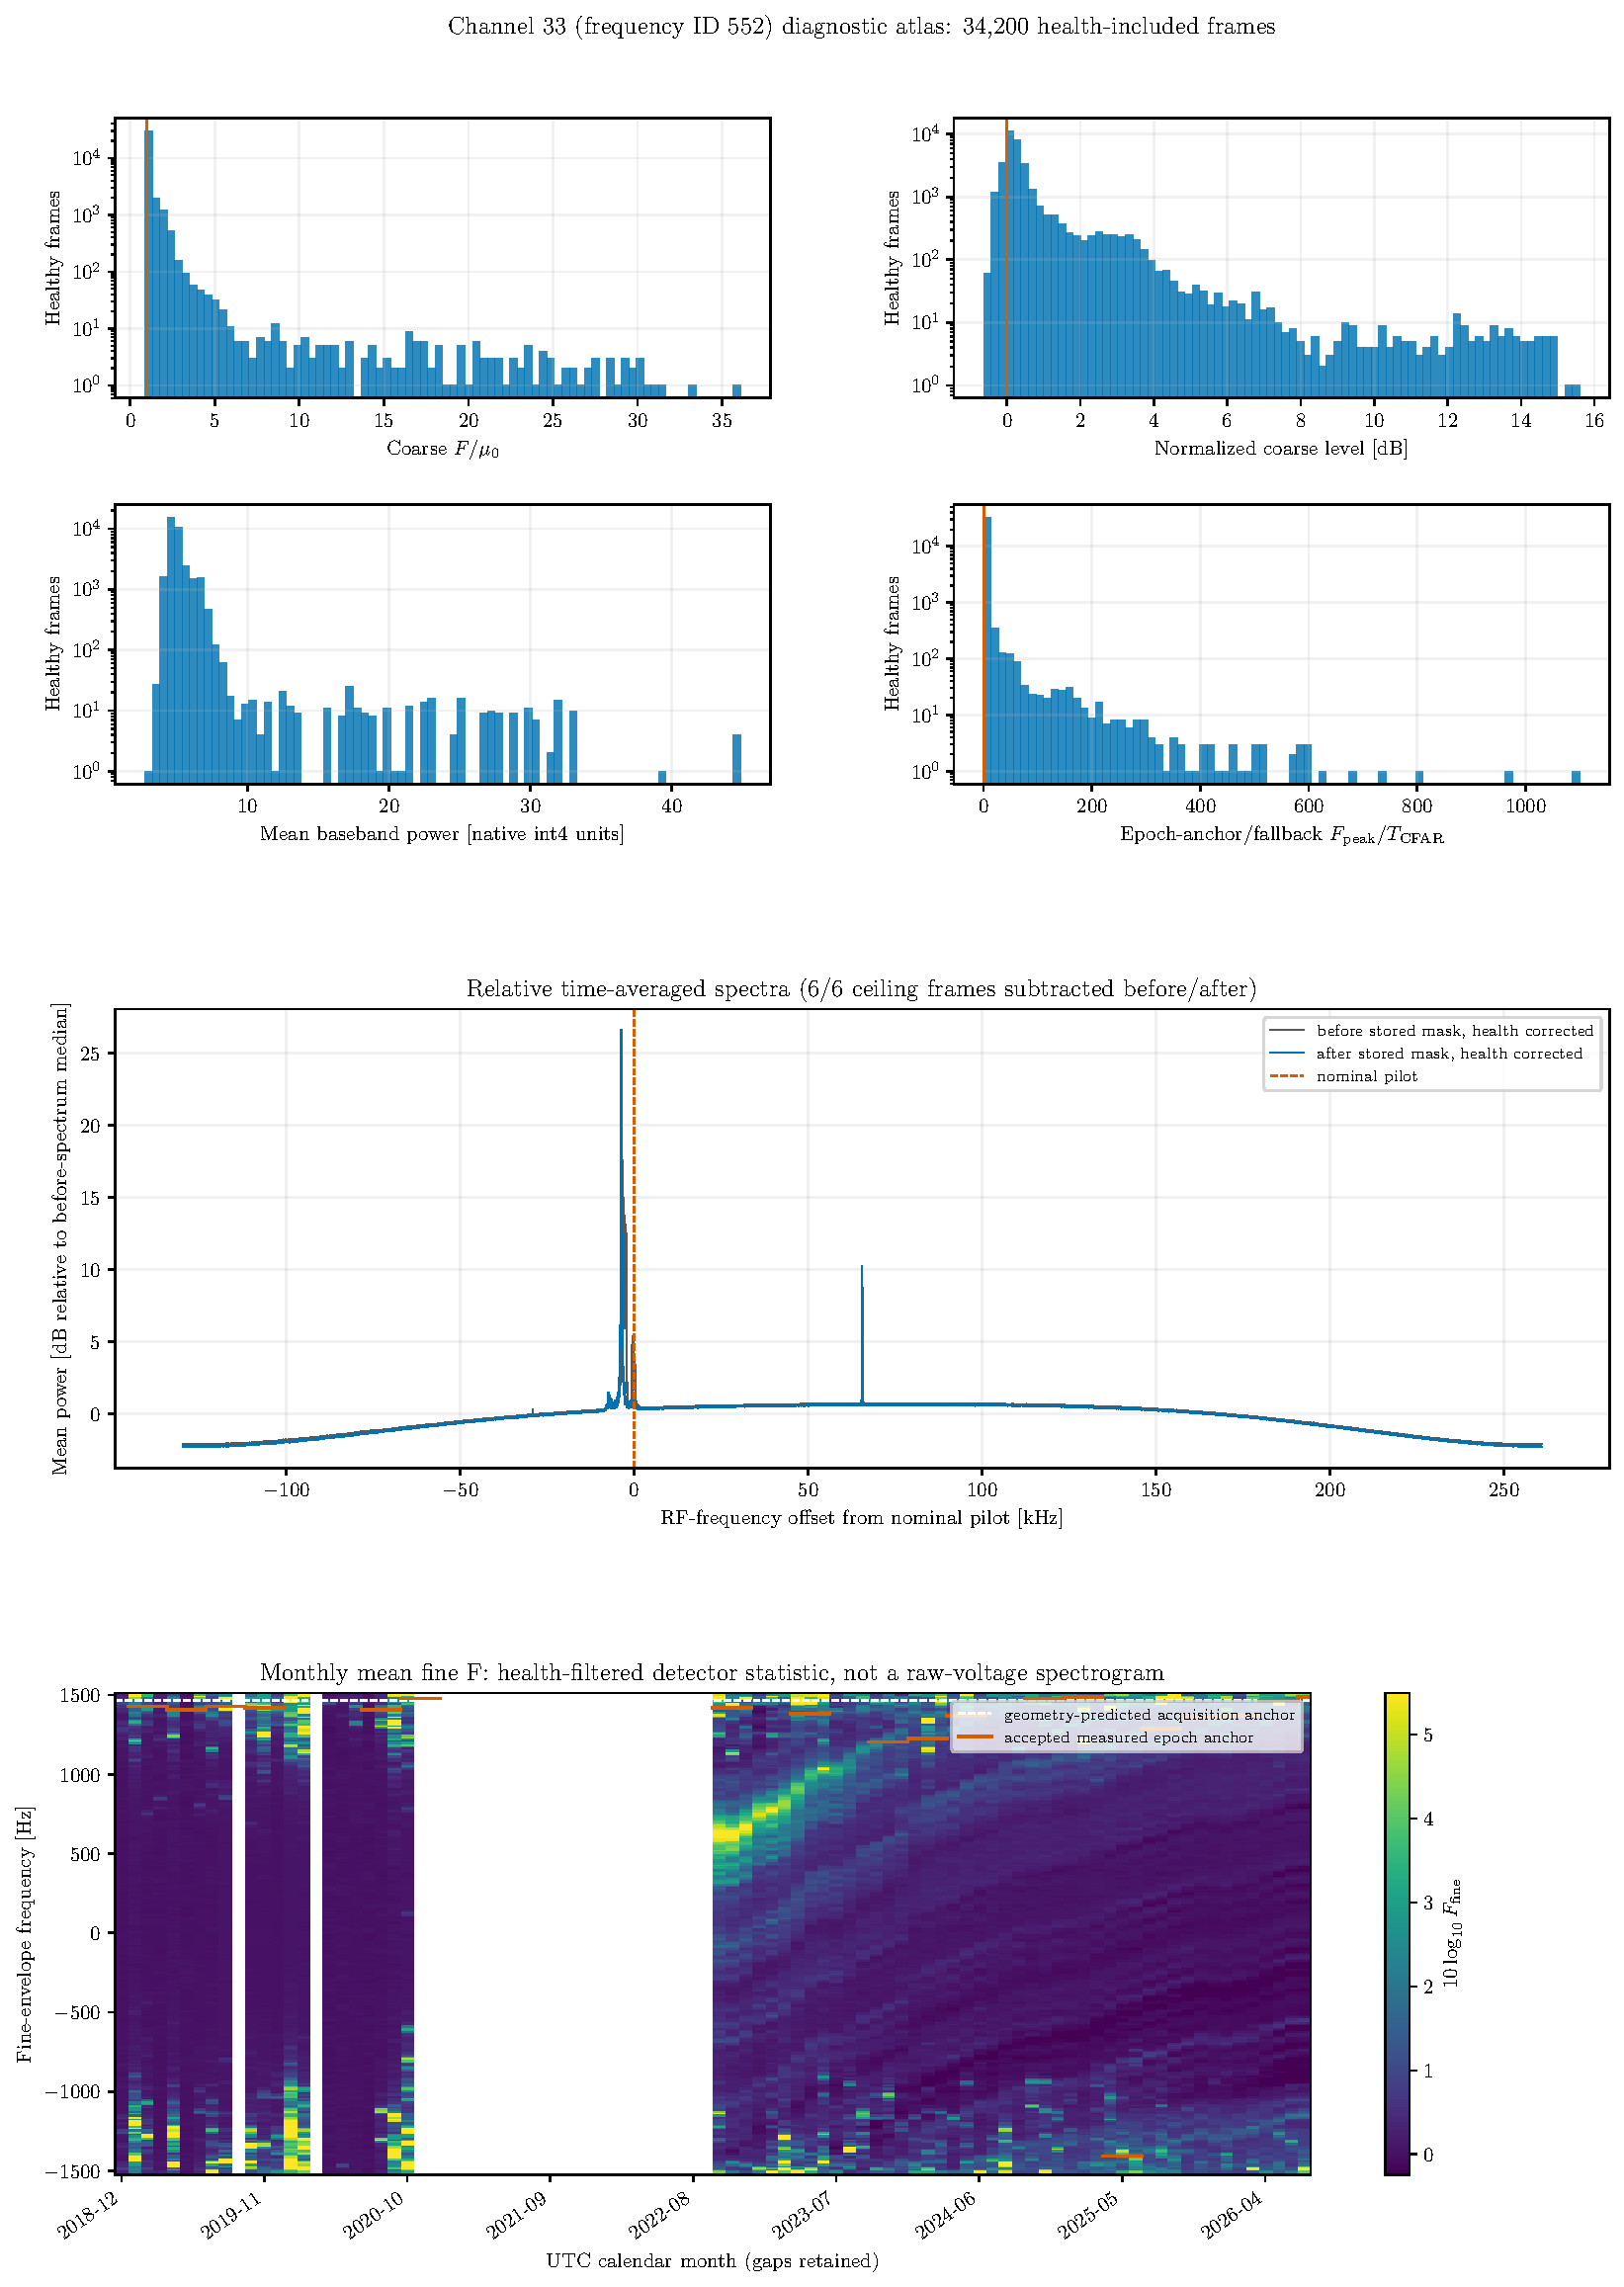
\includegraphics[width=0.98\linewidth,height=0.82\textheight,keepaspectratio]{figs/archive_health_v1/channel_33_diagnostic_atlas.pdf}
\caption{Channel 33 (\texttt{freq\_id}=552).  Its fine-statistic structure is broader than a single narrow anchor, so the heatmap is evidence for diagnosis rather than permission to claim the full fine-stage gain.}
\label{fig:archive:atlas:33}
\end{figure}
\clearpage

\begin{figure}[p]
\centering
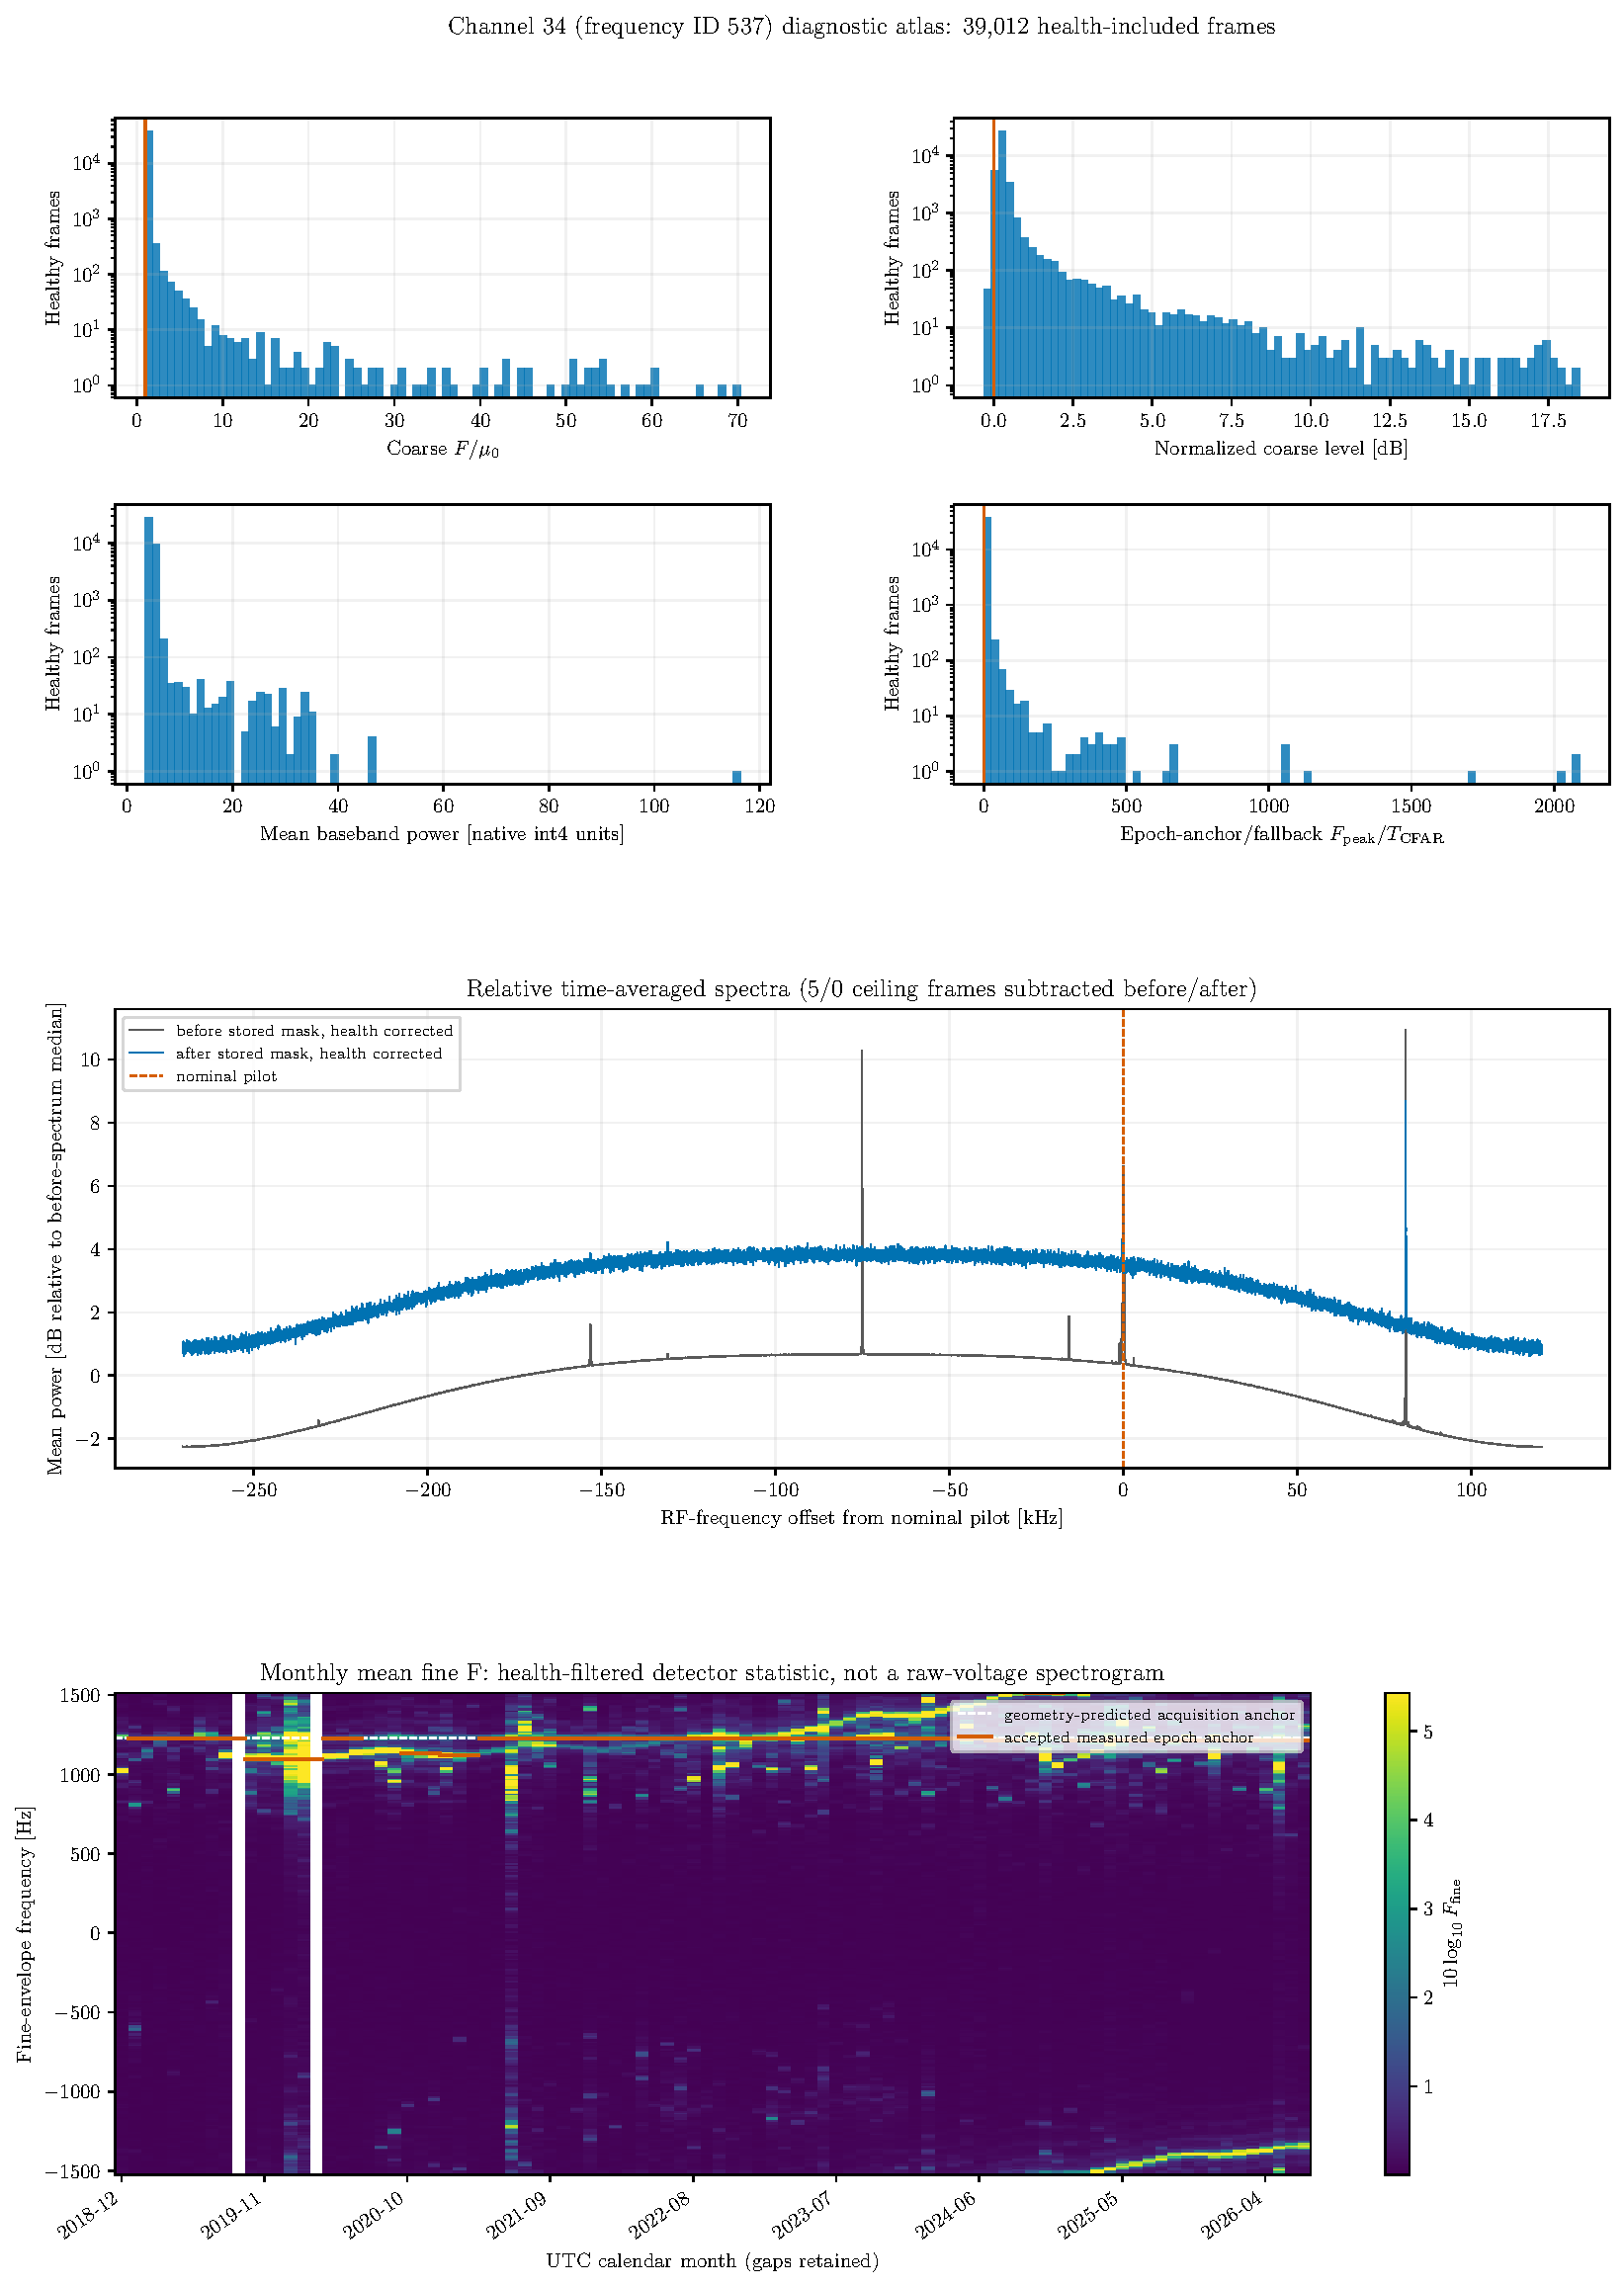
\includegraphics[width=0.98\linewidth,height=0.82\textheight,keepaspectratio]{figs/archive_health_v1/channel_34_diagnostic_atlas.pdf}
\caption{Channel 34 (\texttt{freq\_id}=537) health-filtered archive diagnostics.}
\label{fig:archive:atlas:34}
\end{figure}
\clearpage

\begin{figure}[p]
\centering
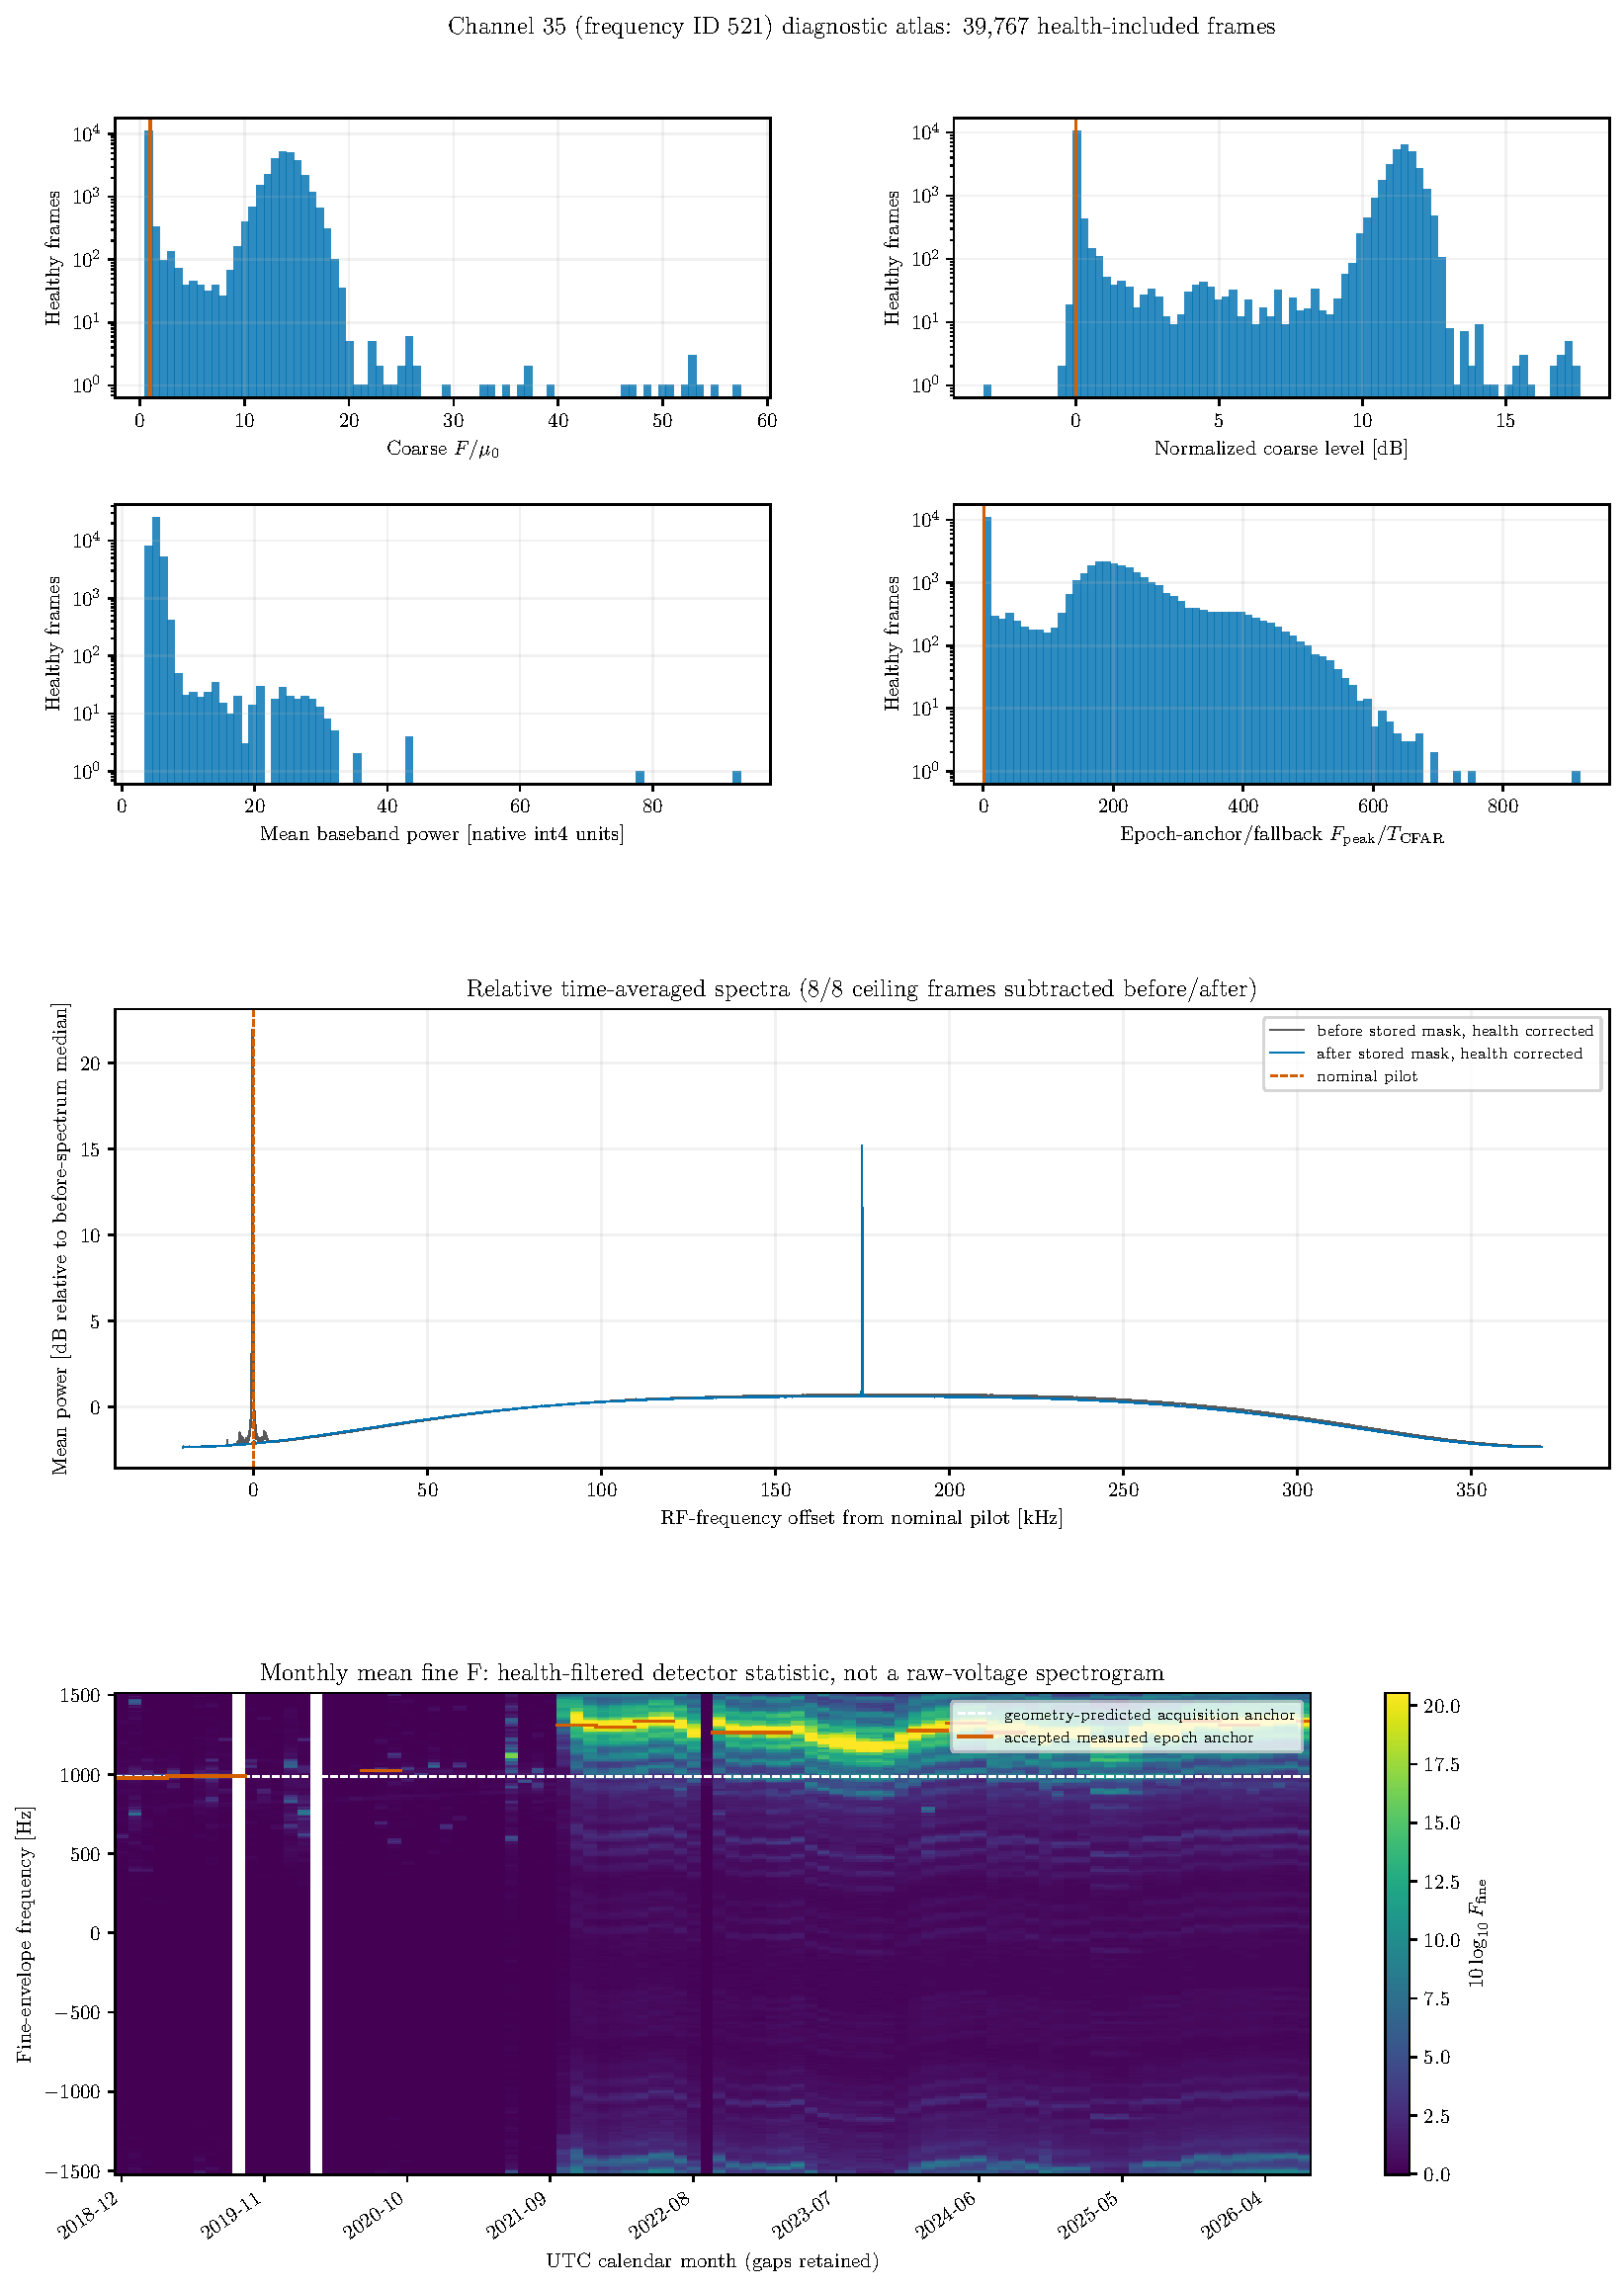
\includegraphics[width=0.98\linewidth,height=0.82\textheight,keepaspectratio]{figs/archive_health_v1/channel_35_diagnostic_atlas.pdf}
\caption{Channel 35 (\texttt{freq\_id}=521) health-filtered archive diagnostics.}
\label{fig:archive:atlas:35}
\end{figure}
\clearpage

\begin{figure}[p]
\centering
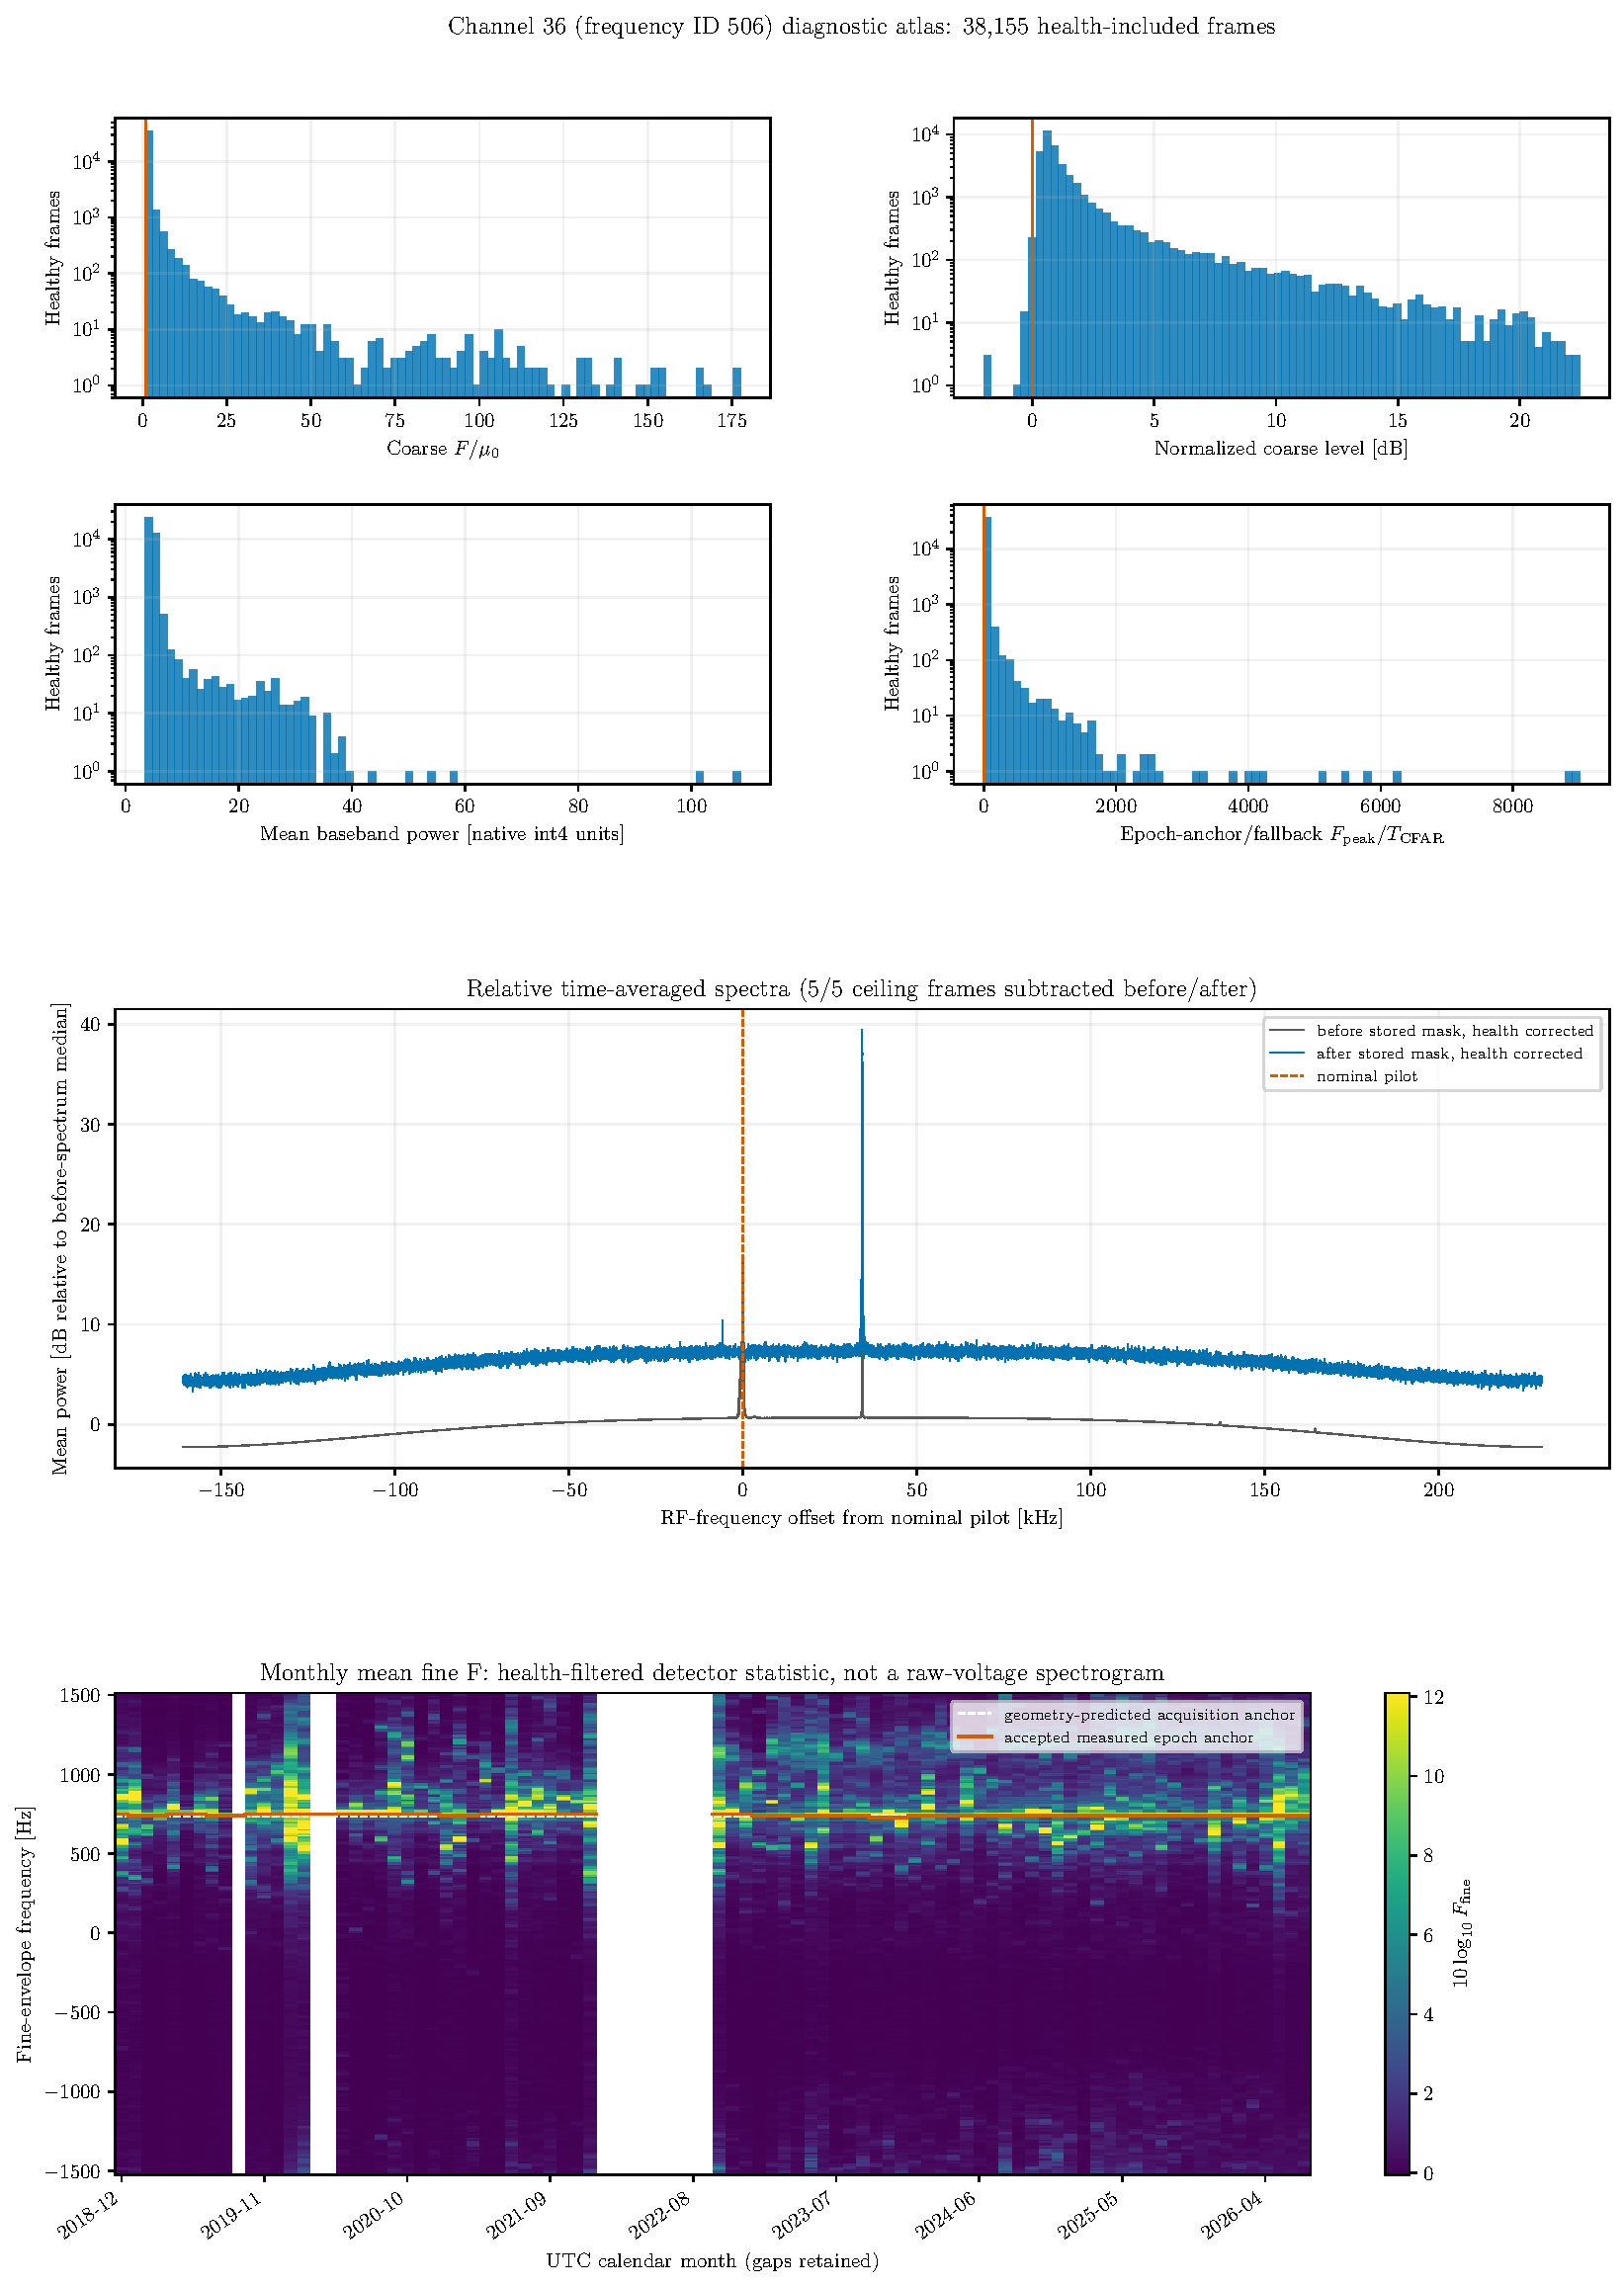
\includegraphics[width=0.98\linewidth,height=0.82\textheight,keepaspectratio]{figs/archive_health_v1/channel_36_diagnostic_atlas.pdf}
\caption{Channel 36 (\texttt{freq\_id}=506) health-filtered archive diagnostics.}
\label{fig:archive:atlas:36}
\end{figure}
